\documentclass[12pt,a4paper]{report}

\usepackage{enumitem}
\usepackage[utf8x]{inputenc}
\usepackage[francais]{babel}
\usepackage[T1]{fontenc}
\usepackage{amsmath}
\usepackage{amsfonts}
\usepackage{amssymb}
\usepackage[square,sort,comma,numbers]{natbib}
\usepackage[colorlinks=true,linkcolor=blue]{hyperref}
\usepackage{glossaries}
\usepackage[usenames,dvipsnames]{xcolor}
\usepackage{setspace}
\usepackage{graphicx}
\usepackage[rightcaption]{sidecap}
\usepackage{subfigure}
\usepackage{float}
\usepackage[skip=2pt,font=scriptsize]{caption}
\usepackage{listings}
\usepackage{xcolor}
\usepackage[top=2cm, bottom=3cm, left=2cm , right=2cm]{geometry}
\usepackage{multirow}
\usepackage{colortbl}

\author{Nicolas JEANNE}
\title{Rapport de stage de M2}
\date{11 mars 2015}

% Mise en page des citations
\bibliographystyle{abbrvnat}
\setcitestyle{authoryear,open={(},close={)},aysep={},citesep={;}}


% formattage des entrées du glossaire
%\renewcommand*{\glstextformat}[1]{\emph{#1}}
% création des acronymes du glossaire
\newacronym{rep}{REP}{Repeated Extragenic Palindrome}
\newacronym{bime}{BIME}{Bacterial Interspesed Mosaic Element}
\newacronym{sra}{\texttt{SRA}}{Sequence Read Archive}
\newacronym{ngs}{NGS}{Next Generation Sequencing}
\newacronym{sam}{\texttt{SAM}}{Sequence Alignment Map format}
\newacronym{bam}{\texttt{BAM}}{Binary Alignment Map format}
\newacronym{gff}{\texttt{GFF}}{General Feature Format}
\newacronym{bed}{\texttt{BED}}{Browser Extensible Data}
\newacronym{de}{DE}{Diff\'erence d'Expression}
\newacronym{rpkm}{RPKM}{Reads Per Kilobase per Million mapped reads}
\newacronym{pdp}{PDP}{Pruned Dynamic Programming}
\newacronym{rig}{RIG}{R\'egion Inter-G\'enique}
\newacronym{et}{ET}{\'Elements Transcriptionnels, tels que les promoteurs et les terminateurs de transcription}

% création des entrées du glossaire
\newglossaryentry{PE}{name={Paired-end sequencing},description={Technique de séquençage haut débit consistant à réaliser les amplifications d'un fragment d'ADN en marquant l'extrémité 5' par un tag \no1 et l'extrémité 3' par un tag \no2. La distance entre les 2 tags est connue et fixe (négative ou jusqu'à 500 pb). Ceci permet lors de l'assemblage, de séquences de 35 pb par exemple, d'associer le read 1 et le read 2 grâce à la distance séparant les 2 et cela même si la séquence intermédiaire est inconnue. Si la distance est négative, il est possible d'obtenir des reads chevauchants de longueur plus importante que les 35 pb}}
\newglossaryentry{SE}{name={Single-end sequencing},description={Technique de séquençage haut débit la plus simple consistant à ne réaliser le séquençage que depuis une extrémité du template.}}
\newglossaryentry{reads}{name={reads},description={Séquence nucléotidique issue d'un séquençage NGS}}
\newglossaryentry{GRanges}{name={Genomic Ranges},description={Format de stockage d'informations pour les éléments génomiques sous R. L'information minimale requise est le chromosome, les positions de départ et de fin, le sens du brin. Ces champs peuvent être suivis de méta-datas où d'autres informations libres peuvent être enregistrées}}
\newglossaryentry{chimerique}{name={alignement chim\'erique},description={Alignement d'un read qui ne peut pas être représenté comme un alignement continu. Un alignement chimérique est représenté comme un ensemble d'alignements, par exemple lorsqu'une partie d'un read est mappé à un locus du génome et la suite à un autre locus}}
\newglossaryentry{couverture}{name={couverture},description={Appelé également profondeur de séquençage, correspond au nombre de reads alignés sur une région génomique. Dans le cas du RNAseq, la couverture fournit une information sur le taux d'expression d'un élément génomique}}
\newglossaryentry{nb}{name={loi Binomiale N\'egative},description={Si une expérience consiste en une série de tirages indépendants  avec une probabilité de succès $p$ et une probabilité d'échec complémentaire, celle-ci se poursuit jusqu'à l'obtention de $n$ succès, la variable aléatoire représentant le nombre d'échecs avant l'obtention des $n$ succès suit une loi négative binomiale. Les paramètres de cette loi sont $n$ le nombre de succès attendus et $p$ la probabilité d'un succès}}
\newglossaryentry{operon}{name={op\'eron},description={unité d'ADN fonctionnelle regroupant des gènes sous le contrôle d'un signal moléculaire régulateur. Les gènes sont transcrits en ARN messager ensemble et concourent à la réalisation d'une même fonction physiologique. Ainsi, soit tous les gènes d'un opéron sont transcrits tous ensemble, soit aucun n'est transcrit puisqu'ils sont tous sous le contrôle du même régulateur}}
\newglossaryentry{tiling-array}{name={tiling-array},description={Cette technique diffère des micro-arrays traditionnels par la nature des sondes, au lieu de disposer de sondes pour des séquences de gènes connues ou prédits, elle sonde des séquences connues pour être disposées dans des régions contiguës et ainsi détecter la présence ou l'absence des transcrits dans ces régions}}
\newglossaryentry{RNA-Seq}{name={RNA-Seq},description={Technique de séquençage haut-débit pour l'étude de l'expression de l'ARN. Un échantillon d'ARN est rétro-transcrit puis amplifié par PCR, le cDNA est séquencé sur un séquenceur haut-débit. Le compte des \gls{reads} produits mappé sur un transcrit représente son abondance}}
\makeglossaries

% Encadrement des figures
\floatstyle{boxed}
\restylefloat{figure}

% Configuration des liens
\hypersetup{
  colorlinks,
  citecolor=Violet,
  linkcolor=Black,
  urlcolor=Blue}

% Configuration des parties de code
\lstset{basicstyle=\small}

\begin{document}

\maketitle

\begin{onehalfspace}
\chapter*{Introduction}
En 1982, la découverte par Higgins de nouveaux éléments génétiques communs dans les régions intercistroniques des opérons de \textit{Escherichia coli} et \textit{Salmonella typhimurium} a constitué le premier pas de la recherche sur les \gls{rep} \citep{Higgins1982}. En 1991, Gilson et al. ont mis en évidence l'organisation en clusters de ces REP \citep{Gilson1991}. Ces clusters ont été appelés \gls{bime}. Chez \textit{E. coli} en 1994, Bachelier et son équipe ont réussi à catégoriser les REP constituant les BIME en 2 types Y et Z, constituants 3 motifs Y, Z\textsuperscript{1}, Z\textsuperscript{2}  \citep{Bachellier1994}.
 
Les REP constituent une part non négligeable du génome bactérien, chez \textit{E. coli K12} ou \textit{S. typhimurium} elles représentent environ 1\% de celui-ci \citep{Gilson1991}. Nous les retrouvons chez de nombreux règnes bactériens, notamment chez les pathogènes humains tels que \textit{Escherichia coli, Salmonella enterica, Neisseria meningitidis, Mycobacterium tuberculosis et Pseudomonas aeruginosa} mais également chez des pathogènes des plantes comme \textit{Agrobacterium tumefaciens} ou chez des bactéries ubiquitaires, \textit{Deinococcus radiodurans} ou \textit{Pseudomonas putida} par exemple. Les travaux précédents de l'équipe ont permis l'annotation des REP au sein des génomes d'\textit{E. coli} et \textit{Shigella} et de mettre en évidence le lien existant entre la prolifération des REP et le gène $tnpA_{REP}$ \citep{Weyder2013,Bosc2014}, ainsi que la reconstruction des états ancêtres des REP \citep{Bosc2014}.  \textcolor{red}{Le rôle exact des REP n'est pas clairement défini, des hypothèses sont avancées sur leur implication dans la régulation de l'expression des gènes, que ce soit en tant que terminateur de transcription ou comme site de reconnaissance des enzymes impliquées dans les mécanismes de la transcription.}

\section*{Caractéristiques des REP et organisations en BIME}

\begin{figure}[ht]
\centerline{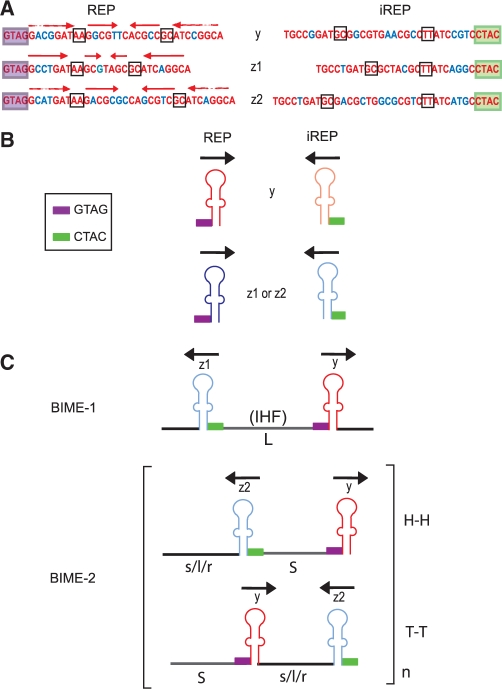
\includegraphics[scale=0.5]{figures/rep_bime.jpg}}
\caption{\textbf{REP et BIME chez \textit{Escherichia coli}. (A)} Séquences consensus Y, Z\textsuperscript{1} et Z\textsuperscript{2} des REP. Le tétra-nucléotide conservé GTAC est encadré en violet, le complémentaire conservé CTAC est encadré en vert, les flèches rouges situent les zones d'appariement de la tige et les positions encadrées en noir sont les zones de mésappariement. Les positions conservées parmi les classes de REP sont en rouge, les positions variables en bleu. \textbf{(B)} Structure secondaire des REP. Les rectangles violets et verts représentent respectivement les tétra-nucléotides conservés GTAC pour les REP et CTAC pour les iREP. Les flèches noires indiquent l'orientation des REP. \textbf{(C)} Structures des BIME-1 et BIME-2. Les BIME-1 sont composées de REP et de iREP Y et Z\textsuperscript{1} séparées par un linker de séquence longue (L), les BIME-2 sont composées de Y et Z\textsuperscript{2}, de linker courts (S) et de séquences séparatrices s, l ou r. H-H et T-T dénotent respectivement une organisation tête à tête et queue à queue des REP. \citep{Ton-Hoang2012}.}
\label{fig:rep_bime} 
\end{figure}

Chez \textit{E. coli}, la taille des REP est d'environ 40 nucléotides, la classification Y, Z\textsuperscript{1}, Z\textsuperscript{2} est basée sur leur séquence primaire. Par convention, une REP en orientation inversée est nommée iREP (inversed REP) \citep{Ton-Hoang2012}. Un tétra-nucléotide caractéristique de séquence GTAC est présent à l'extrémité 5' des REP, sa séquence complémentaire est CTAC en 3' pour les iREP. Les séquences consensus des différentes classes de REP partagent des nucléotides conservés (\autoref{fig:rep_bime}A). La structure secondaire des REP est caractérisée par sa forme en tige-boucle, le caractère palindromique permet la formation de la tige malgré un mésappariement situé dans la partie centrale de celle-ci (\autoref{fig:rep_bime}B) permettant la reconnaissance par $tnpA_{REP}$. Une classification a été adoptée comportant 3 classes \citep{Bachellier1997}, les BIME-1 composées de REP Z\textsuperscript{1} et Y apparaissant en paires uniques. Les BIME-2 constituées de Z\textsuperscript{2} et de Y, apparaissant en copies multiples de cette paire. La troisième catégorie est constituée des BIME dites atypiques qui sont des chimères de BIME-1 et BIME-2, comportant différentes combinaisons de Y, Z\textsuperscript{1}, Z\textsuperscript{2}. Tout comme les BIME-2, nous les retrouvons sous forme de copies multiples (\autoref{fig:rep_bime}C). Les REP peuvent former des structures secondaires avec elles-même, mais également entre elles lorsqu'elles sont organisées sous forme de BIME \textcolor{red}{à quel endroit cette figure? (\autoref{fig:malEF_rep})}.

\begin{figure}[ht]
\centerline{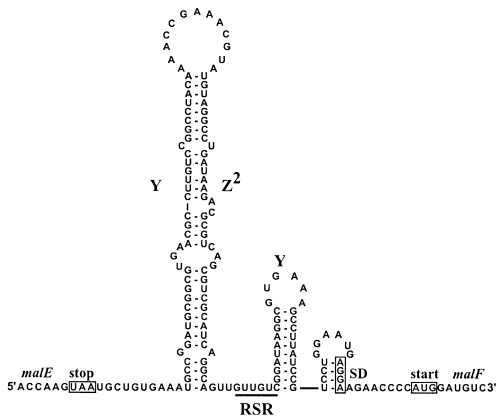
\includegraphics[scale=0.5]{figures/malEF_rep.png}}
\caption{\textbf{Structure ARN des REP au sein de l’opéron \textit{malEFG}.} Y, Z\textsuperscript{2} et Y indiquent la séquence des REP dans l'espace inter-génique de malE-malF. Bien que Y et Z\textsuperscript{2} puissent former des structures tige-boucles par elles mêmes, elles s'apparient ensemble pour former une région étendue en grande partie à double brin (70\% des nucléotides sont appariés). La séquence affichée provient du génome d'\textit{E. coli K12}. La région REP-stabilized RNA (RSR) indique l'extrémité 3′ du messager malE mature, qui s'étend de 3 à 9 nucléotides depuis la base de la tige-boucle formée par Y et Z\textsuperscript{2}. Les codons STOP de  malE et START de malF sont encadrés. SD représente la séquence Shine–Dalgarno nécessaire à l'initiation de la traduction de malF. \citep{Khemici2004}.}
\label{fig:malEF_rep} 
\end{figure}

\section*{Propriétés associées aux REP}
La littérature décrit de nombreuses fonctions hypothétiques associées aux REP au niveau structurel du génome, au niveau de l'ADN et au niveau de l'ARN. Sur un plan structurel, les REP ont été décrites comme jouant un rôle dans les événements de \textbf{recombinaisons homologues} \citep{Kofoid2003} et les BIME ont été décrites comme des sites privilégiés pour \textbf{l'insertion de séquences d'ADN mobiles} comme certaines familles d'IS (Insertion Sequence) \citep{Bachellier1997,Clement1999,Choi2003,Tobes2005}. Au niveau de l'ADN, les REP sont capables de \textbf{lier plusieurs facteurs protéiques} tels que l'ADN Gyrase \citep{Espeli1997} et l'ADN polymérase \citep{Gilson1990}. Plus spécifiquement, la BIME-1 peut \textbf{lier l'\textit{IHF} sur son linker} \citep{Boccard1993} qui peut être notamment responsable de l'\textbf{initiation de la transcription et d’événements de recombinaisons sites spécifiques} \citep{Goosen1995}. Au plan de l'ARN, lorsqu'elles sont transcrites, les REP joueraient un rôle dans la \textbf{stabilisation de l'ARNm} grâce à leur structure en tige-boucle \citep{Newbury1987,Espeli2001,Khemici2004,Aguena2009}, la \textbf{terminaison de la transcription} \citep{Gilson1986} et \textbf{le contrôle de la traduction} \citep{Stern1988}. 

\section*{ARN messagers chez \textit{E. coli}}

\subsection*{Stabilité des ARNm}
La dégradation des ARNm chez \textit{E.coli} est réalisée par l'intervention du dégradosome. Il s'agit d'un complexe multi-enzymatique composé de quatre protéines majeures, la RNase E, la PNPase, la RhlB et l'Enolase (\autoref{fig:degradosome}).

\begin{figure}[ht]
\centerline{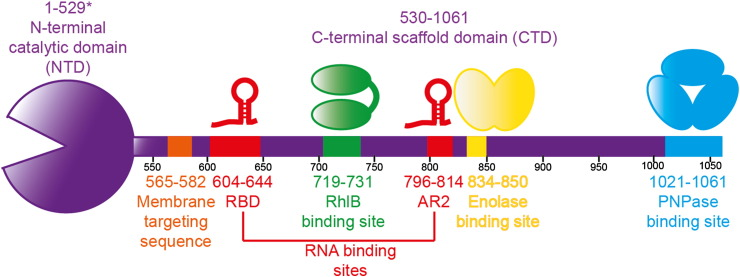
\includegraphics[scale=4]{figures/degradosome.jpg}}
\caption{\textbf{Structure du dégradosome.} Représentation canonique du dégradosome, la partie violette symbolise la RNase E avec le domaine catalytique à gauche, la partie verte le site de liaison de la RhlB, la jaune celui de l'Enolase et la bleue celui de la PNPase \citep{Bandyra2013}.}
\label{fig:degradosome} 
\end{figure}

Un élément clé dans la dégradation du transcrit chez \textit{E. coli} est que celle-ci débute toujours par un clivage réalisé par une endoribonucléase (RNase E). Une fois clivés, les transcrits sont complètement dégradés par des exoribonucléases (RNase R, RNase II ou PNPase) dégradant l'ARNm par l'extrémité 3' et par des oligoribonucléases grâce à la coopération de nombreuses enzymes telles que la poly(A) polymérase (PAP) et les RNA hélicases qui facilitent l'accès aux fragments d'ARN. La RNase E possède une affinité pour les substrats possédant une extrémité mono-phosphate en 5'. Les transcrits primaires bactériens possèdent une extrémité 5' tri-phosphate qui les protège de la dégradation jusqu'à ce qu'ils soient déphosphorylés par l'activité des pyrophosphohydrolases. La RNAse E reconnaît alors l'extrémité 5' mono-phosphate des transcrits par contact de son domaine catalytique \citep{Callaghan2005,Bandyra2013}.

\begin{SCfigure}[][h!]
\fbox{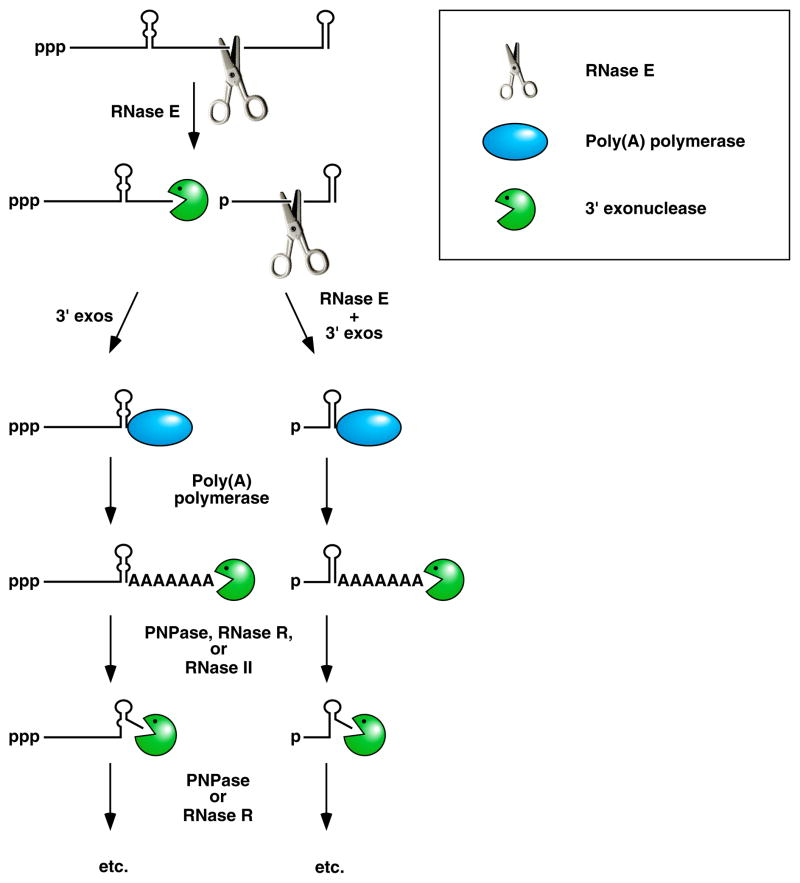
\includegraphics[scale=0.65]{figures/mrna_degradation.jpg}
\caption{\textbf{Facilitation de la dégradation des ARNm chez E. coli par l'intervention de polyadénylation.} Le clivage endonucléolytique par la RNase E génère de multiples fragments, dont certains possèdent à leur extrémité 3' une structure en tige-boucle. Ces fragments subissent une digestion de leur extrémité 3' par la PNPase, la RNase II et/ou la PNPase jusqu'à ce que cette structure soit rencontrée interrompant la dégradation. La PAP intervient pour déstabiliser la tige boucle par l'ajout d'une séquence poly-A en 3' autorisant la reprise de la dégradation par la PNPase et/ou la RNase R \citep{Belasco2010}.}
\label{fig:mrna_degradation} }
\end{SCfigure}

La présence de structure secondaires peut entraver le processus de dégradation initié par les exoribonucléases, la PAP intervient alors en ajoutant sur l'extrémité 3' du transcrit une séquence poly-A qui va déstabiliser la structure secondaire et permettre ainsi aux exoribonucléases de poursuivre la dégradation (\autoref{fig:mrna_degradation}).

\subsection*{Terminaison de la transcription}
Le mécanisme de terminaison de la transcription chez les procaryotes est gouverné par deux classes signaux de fin de transcription. Les terminateurs Rho-dépendant dont l'activité s'appuie sur la liaison de la protéine Rho à un site \emph{rut} (Rho utilization) présent sur le transcrit associé à une interaction avec la RNA Polymérase et les terminateurs Rho-indépendants caractérisés par une structure G-C riche formant une tige-boucle suivie d'une série de résidus U. Ces terminateurs peuvent être bi-directionnels (\autoref{fig:terminator}) \citep{Henkin2000,Lesnik2001}.  

\begin{SCfigure}[][h!]
\fbox{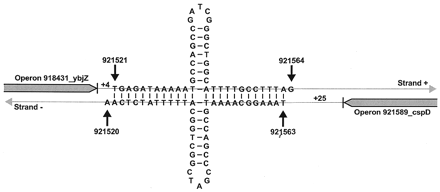
\includegraphics[scale=0.65]{figures/terminator.png}
\caption{\textbf{Terminateur Rho-indépendant bi-directionnel.} La région riche en G-C constitue la structure en tige, la boucle étant formée par les bases non appariées. A la suite de cette structure, nous observons la répétitions de T (U) caractéristique. \citep{Lesnik2001}.}
\label{fig:terminator} }
\end{SCfigure}


\vspace{2.8cm}Dans l'état actuel de la recherche beaucoup de pistes pointent vers le fait que les REP joueraient un rôle soit dans la terminaison de la transcription, soit dans le processus de dégradation des \textcolor{red}{transcrits au niveau ARN CITER REFERENCE ou protéique CITER REFERENCE}. Plusieurs technologies sont disponibles pour étudier l'expression des gènes, les principales sont le micro-array, le \gls{tiling-array} et le \gls{RNA-Seq}. Notre choix s'est porté sur le RNA-Seq car il présente plusieurs avantages sur les autres technologies. A la différence des arrays, cette technologie ne nécessite pas la synthèse de sondes spécifiques des espèces ou des transcrits, elle peut donc détecter de nombreux événements non attendus. Elle offre des seuils de détection beaucoup plus bas car elle ne souffre pas du bruit spécifique aux arrays ce qui améliore sa spécificité et sa sensibilité. Sa profondeur de séquençage permet de détecter des transcrits rares et de faible abondance.

Concernant le RNA-Seq, nous pouvons distinguer deux approches. L'une classique qui consiste à analyser les données d'expression de mutants par rapport à un individu sauvage (Wild-Type WT) ou une population dans des conditions classiques et une population dans des conditions perturbées. Et l'autre, alternative, où pour une même condition, nous nous intéressons à la \textbf{différence de niveau d'expression d'un gène par rapport à un autre}. Classiquement dans le cas d'un \gls{operon}, nous nous attendons à ce que les gènes qui le constituent aient un profil d'expression similaire. Cette approche est privilégiée pour notre étude puisque nous cherchons à déterminer le rôle des REP dans la régulation de la transcription.
A notre connaissance, il n'existe pas d'approche globale sur l'implication des REP dans la transcription, nous avons développé des méthodes pour tenter de découvrir le rôle des REP en nous basant sur des données d'expressions issues d'expériences de RNA-Seq.


\chapter*{Matériel \& Méthodes}

\section*{Fichiers d'annotations}
Le fichier \gls{gff} d'annotation du génome d'\textit{E. coli K12} a été généré par un script Perl à partir du fichier \href{http://www.ncbi.nlm.nih.gov/nuccore/NC_000913.2}{GenBank}. Les fichiers répertoriant les opérons et les promoteurs proviennent de \href{http://regulondb.ccg.unam.mx/}{RegulonDB}. Pour les opérons, le fichier se compose de 2640 entrées dont 848 sont des opérons de plus d'un gène et parmi ces derniers, 235 ont été annotés comme ayant de fortes preuves de leur existence (expérimentalement vérifiés), les 613 autres présentent des preuves d'existence plus faibles (inférence automatique, bibliographie\ldots). Le fichier des promoteurs contient 8580 entrées dont 6461 ont été annotées comme présentant des preuves fortes d'existence. Le fichier répertoriant les terminateurs de transcription provient de \href{http://csbl.bmb.uga.edu/DOOR/}{Door\up{2}DB}) et contient 1835 entrées, nous n'avons pas d'information quand à la manière dont ils ont été annotés. Quand aux REP et BIME, les fichiers d'annotations proviennent de l'équipe \textcolor{red}{\textbf{Donner la façon dont ils ont été annotés}}.

\section*{Données}
Plusieurs jeux de données ont été utilisés, tous issus d'expériences RNA-Seq publiques, accessibles sur le base de données \href{http://www.ncbi.nlm.nih.gov/geo/}{GEO} (Gene Expression Omnibus) du NCBI au format \gls{sra}. Grâce au \href{http://www.ncbi.nlm.nih.gov/books/NBK158900/#SRA_download.how_do_i_use_the_sra_toolki}{SRA toolkit} elles sont décompressées au format \texttt{fastq} et un contrôle de qualité est effectué afin d'inspecter les \gls{reads} grâce au logiciel \texttt{fastqc} (Annexe \ref{annexeCode}).

Le \href{http://www.ncbi.nlm.nih.gov/geo/query/acc.cgi?acc=GSE61327}{premier jeu de données} que nous avons exploité est issu des expériences d'évolution adaptatives en laboratoire visant à découvrir l'émergence de mutations clés permettant la croissance rapide d'\textit{E. coli K-12 MG1655} sur un medium pauvre en glucose \citep{Lacroix2014}. Ces données ont été choisies car elles proviennent d'expériences de RNA-Seq comportant un nombre important de réplicats (9) pour la condition de croissance en milieu pauvre en glucose (GSE61327\_ALE) et 2 réplicats pour le Wild Type (WT) , mais nous n'avons exploité que la condition ALE, le nombre de réplicats du WT étant faible. Elles ont été obtenues par séquençage sur Illumina MiSeq à partir d'ARN total extrait des cultures d'\textit{E. coli} et rétro-transcrit en cDNA. La librairie a été conçue en \gls{PE}. 8 réplicats ont été validés disposant d'une qualité de séquence par base supérieure à 30 pour des reads de 62 pb, seul le fichier \texttt{SRR1573441.fastq} a été rejeté car la longueur des reads allait de 35 à 502 pb avec des scores de qualités très variables.

Le \href{http://bioinfolab.uncc.edu/TruHmm_package/raw_data/}{second jeu de données} provient d'une expérience visant à développer un algorithme pour la détection des opérons chez \textit{E. coli K12} \citep{Li2013}. Nous nous sommes intéressés à celles provenant des cultures ayant subi un choc thermique pendant 15 minutes (HS-15min) ainsi qu'à celles provenant de culture privées de phosphore pendant 4 heures (M-P4h). Ces 2 conditions ont été retenues car elles possèdent 3 réplicats contre 2 pour toutes les autres. Les librairies ont été conçues en \gls{SE} et brin spécifique en utilisant le kit Illumina’s TruSeq Small RNA Sample Prep, puis séquencées à la fois sur Illumina HiSeq 2000 (générant des reads de 100 bases) et Illumina GA II (générant des reads de 76 bases). Aucun réplicat n'a été rejeté suite aux contrôles qualité.

\section*{Alignement des reads}
Les reads ont été alignés puis mappés sur le génome d'\textit{E. coli} \href{http://www.ncbi.nlm.nih.gov/nuccore/NC_000913.2}{NC\_000913.2}, qui est le génome utilisé pour annoter les REP par l'équipe, grâce au logiciel \href{http://bio-bwa.sourceforge.net/}{BWA}.  Ce logiciel propose 3 algorithmes distincts, BWA-backtrack, BWA-SW et BWA-MEM. Pour chacun de ces alignements, il est nécessaire de disposer de la séquence du génome de référence indexée, obtenue par la commande \texttt{bwa index NC\_000913.2.fasta}. 
L'algorithme que nous avons sélectionné est le \texttt{MEM} (Maximal Exact Matches) pour sa rapidité et sa précision. Il reprend les mêmes principes que \texttt{BWA-SW} (utilisation de la programmation dynamique pour trouver les points d'ancrage (seeds) en autorisant les mésappariements (mismatchs) et les brèches (gaps). Il n'étend les alignements des seeds que lorsque ceux-ci ont peu d'occurrences sur le génome de référence, cela permet de diminuer le temps d'alignement en éliminant les extensions des séquences très répétées) mais en utilisant l'ancrage avec des \texttt{MEM}, puis il réalise l'extension en prenant en compte les pénalités dues aux gaps et aux mismatchs. Les valeurs par défaut du logiciel ont été utilisées (Annexe \ref{annexeCode}).
Le fichier d'alignement généré est au format \gls{sam}, afin de poursuivre l'analyse il doit être converti au format \gls{bam}, puis des critères de qualité sont appliqués. Seules les séquences possédant une qualité de mapping > 30, valeur d'usage commun, et n'étant pas étiquetées (taggées) comme \gls{chimerique} sont conservées. Cette opération a aussi le mérite de compresser l'information et ainsi de gagner en espace de stockage. Les séquences sont ensuite triées par position génomique. Finalement, le fichier BAM trié est indexé pour être visualisable sur un Genome Browser. Les outils utilisés sont compris dans la suite des \href{http://samtools.sourceforge.net/samtools.shtml}{samtools}. Pour les besoins ultérieurs de l'analyse, les réplicats d'une même condition sont fusionnés en un seul fichier (Annexe \ref{annexeCode}).

\subsection*{Intégration des données}
Les fichiers d'annotation ont été transformés au format \gls{bed} grâce à des scripts Python.
Ces changements de format permettent de travailler aisément avec la suite de logiciels \href{http://bedtools.readthedocs.org/en/latest/}{BEDtools} permettant de croiser les informations provenant de plusieurs sources de données et ainsi de rechercher des intersections, des positions proches ou déterminer une \gls{couverture} de reads. Ces outils ont généré les fichiers \texttt{BED} qui serviront de référence pour la suite de l'analyse statistique.

\subsection*{Visualisation du mapping}
L'alignement des reads et le mapping sur le génome de référence de \textit{E. coli} sont visualisés grâce au genome browser \href{https://www.broadinstitute.org/igv/}{IGV} \citep{Robinson2011,Thorvaldsdottir2013} (\autoref{fig:igv}).

\begin{figure}[h!]
\centerline{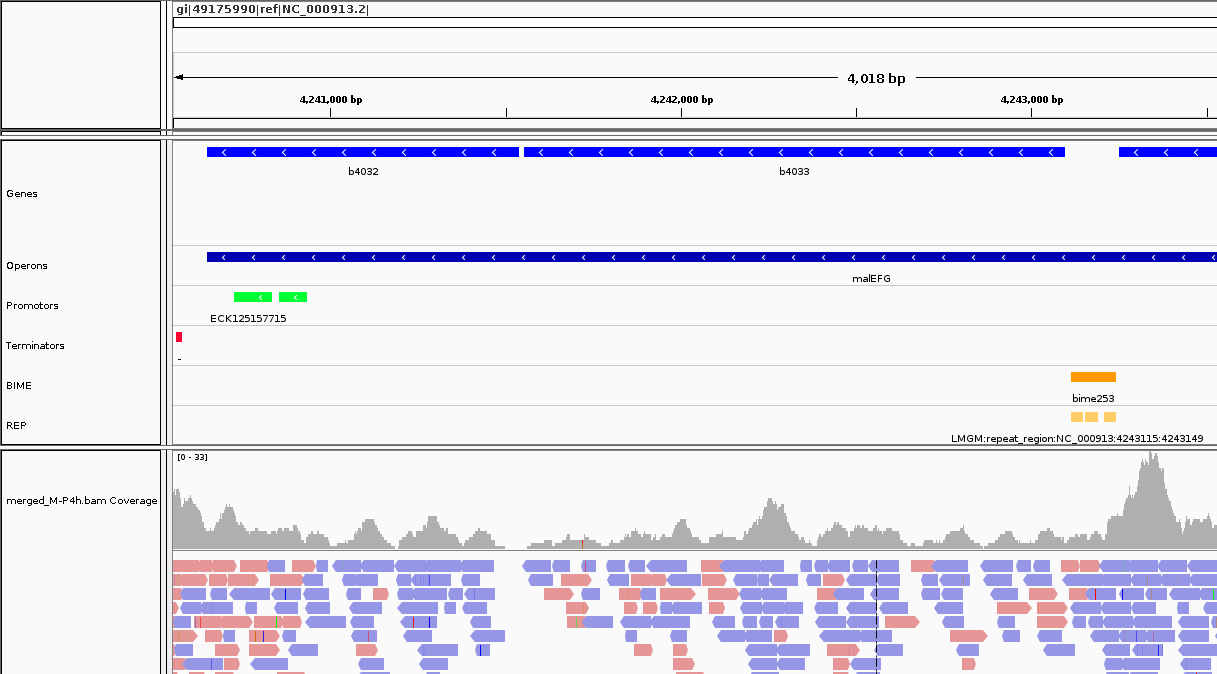
\includegraphics[scale=0.4]{figures/igv_snapshot.png}}
\caption{\textbf{Visualisation du mapping de l'opéron malEFG sur IGV.} Les premières pistes représentent les positions et orientations des gènes, des opérons, la présence de promoteurs et de terminateurs, ainsi que la position des BIME et des REP qui composent les BIME. Les 2 pistes suivantes affichent la couverture des fichiers \texttt{BAM} fusionnés de la région visualisée (histogramme gris) et l'alignement des reads (flèches pleines rouges et bleues). La couleur bleue sur cette piste indique un alignement sur le brin direct et la couleur rouge sur le brin complémentaire.}
\label{fig:igv} 
\end{figure}

\section*{Création de la table de comptages et normalisation}
Afin d'obtenir des résultats de comptage par région d'intérêt et ainsi estimer l'expression, nous avons utilisé le package Bioconductor easyRNASeq \citep{Delhomme2012} puisqu'il permet de réaliser les opérations de comptage de façon documentée et qu'il offre la possibilité d'effectuer une normalisation par \gls{rpkm}. Les annotations du génome d'\textit{E. coli} relatives aux gènes sont extraites à partir du fichier \texttt{GFF} et stockées sous forme d'une base de données. Cela a nécessité une manipulation préalable de ce fichier, en effet les opérons récupérés sur RegulonDB sont composés à la fois de gènes dont les transcrits sont annotés ARNm, ARNt et ARNr. Seul les gènes dont le transcrit est annoté ARNm est pris en compte par le package easyRNASeq, donc pour ne pas avoir d'erreur dans l'analyse, nous avons transformé les annotations ARNt et ARNr en ARNm.
La liste des transcrits par gène est ensuite extraite pour un total de 4605 éléments que nous nommerons régions. La couverture par région est ensuite calculée pour chaque fichier \texttt{BAM}, le résultat est obtenu en réalisant l'union des positions extraites de la liste des régions et des positions des reads extraites des fichiers BAM qui auront été préalablement transformées au format \gls{GRanges} (\texttt{GRanges})  \citep{Lawrence2013}. Une table de comptage est alors produite, les régions figurant en ligne et les fichiers BAM en colonnes.

Les résultats de comptages doivent ensuite être normalisés afin de permettre la comparaison de l'expression des gènes et des régions génomiques d'intérêt. De nombreuses méthodes de normalisation existent dont certaines introduisent un biais notamment pour la recherche de DE. La méthode du RPKM reflète la concentration molaire du transcrit en normalisant par la longueur du brin d'ARN et le nombre de reads de la bibliothèque. Cette normalisation est soumise à critique à juste titre \citep{Dillies2013} car elle induit un biais de lors d'une analyse de DE dans le cas de gènes fortement exprimés dans un condition par rapport aux autres conditions. Comme nous ne nous situons pas dans le cadre d'une analyse différentielle sur plusieurs conditions, mais que nous comparons des réplicats d'une même condition, nous pouvons appliquer cette normalisation. Notre choix s'est porté donc porté sur cette méthode \citep{Mortazavi2008} :

\[RPKM = Nb.~reads~transcrit~*~\frac{1000~bases~*~10^6}{Nb.~total~reads~*~Taille~du~transcrit}\]

\textcolor{red}{Il faut souligner que comme nous ne nous intéressons pas à un même gène dans 2 conditions différentes mais à 2 gènes dans une même condition, un biais dû à leur composition en GC peut intervenir.}

Les données sur lesquelles nous allons travailler sont issues de la table de comptage et ont subi une normalisation, afin de vérifier que l'homogénéité entre les réplicats est toujours présente, nous réalisons une analyse en composante principale. Le déroulé de l'analyse pour produire la table de comptage normalisée est représenté sur la \autoref{fig:data_preparation}.

\begin{figure}[h!]
\centerline{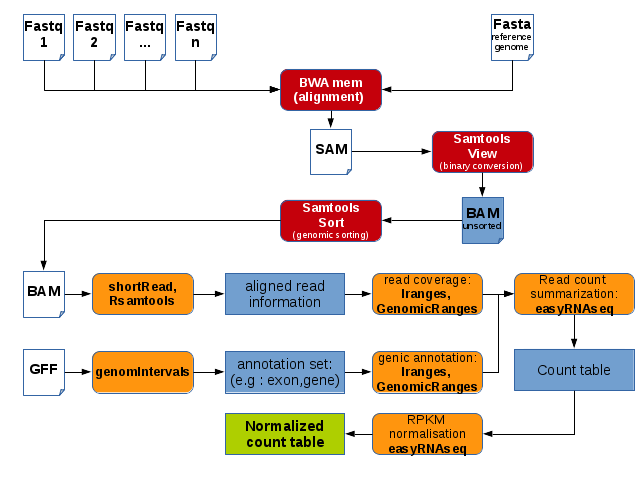
\includegraphics[scale=0.9]{figures/data_preparation.png}}
\caption{\textbf{Pipeline de l'analyse pour obtenir la table de comptage normalisée.} Pour le modèle choisi sur notre analyse, les fichiers d'entrée sont en blanc, les traitements avec des logiciels externes à \texttt{R} sont en rouge, les traitements par les packages \texttt{R} sont colorés en orange, les données intermédiaires en bleu et la table de comptage normalisée produite est en vert.}
\label{fig:data_preparation} 
\end{figure}

\section*{Corrélation de profils d'expression}
\label{methode_correlation}
Le principe de cette analyse repose sur la recherche de corrélation entre le profil d'expression issu de données de RNA-Seq et un profil simulé représentant un changement de niveau d'expression, cette méthode a été mise au point pour la prédiction d'opérons dans les génomes bactériens \citep{Fortino2014}. Le concept général est de délimiter les bornes des transcrits à partir de données de couverture en s'appuyant sur un test de corrélation entre ce profil et un profil simulé de 0 et de 1. Les 0 représentant une zone sans couverture donc en dehors d'un transcrit et les 1 la zone couverte, donc le transcrit. Le cœur de leur méthode consiste à déplacer une fenêtre glissante de 100 pb parcourant base à base le génome en réalisant des tests de corrélation entre le profil d'expression réel et le profil d'expression simulé par le vecteur de même taille contenant un nombre égal de 0 et de 1 (si l'on cherche une croissance d'expression en sens ou une décroissance d'expression en anti-sens, e.g: 000111), ou de 1 et de 0 (dans le cas d'une décroissance en sens et d'une croissance en anti-sens, e.g: 111000). Les moyennes du taux de couverture sont calculées sur les parties gauche et droite de la fenêtre pour dans un premier temps filtrer les données, le $Log_2$ du rapport de ces moyennes doit être supérieur à 1 ce qui représente un changement de 2 fois du niveau d'expression. Si ce 1\up{er} filtre est passé, la corrélation entre le profil réel et celui simulé est calculée et doit être supérieure à un seuil avec une p-valeur significative (\autoref{fig:profil}) pour être validée. Les auteurs ont fixé un seuil de corrélation de 0.7 et une p-value de $10^{-7}$ comme seuil significatif pour le test de corrélation.

\begin{figure}[ht]
\centerline{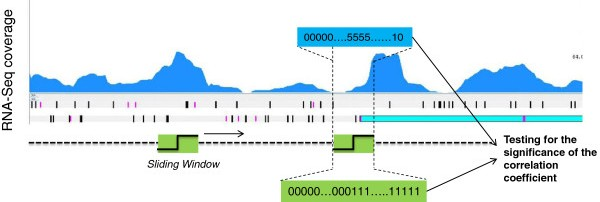
\includegraphics[scale=0.6]{figures/profil.jpg}}
\caption{\textbf{Recherche de corrélation sur des profils d'expression.} La fenêtre glissante (en vert) parcourt la région d'intérêt et pour chaque déplacement une corrélation est calculée entre le vecteur du profil d'expression obtenu par RNAseq (en bleu) et celui simulé par le vecteur de 0 et de 1 (en vert) \citep{Fortino2014}.}
\label{fig:profil} 
\end{figure}

\section*{Segmentation}
\label{methode_segmentation}
A la différence de la méthode précédente, la segmentation ne requière pas l'utilisation de profils. La méthode de segmentation que nous utilisons est issue du package R \href{http://cran.r-project.org/web/packages/Segmentor3IsBack/index.html}{Segmentor3IsBack} \citep{Cleynen2014}. Le but de cette méthode est de rechercher, sur une zone d'intérêt, des points de changements abrupts dans la couverture en utilisant l'algorithme \gls{pdp} \citep{Rigaill2010}. La segmentation se fonde sur le partitionnement d'un signal de $n$ points, la couverture de notre région d'intérêt, compris dans l'ensemble ${\{y_t\}_{t=1,\ldots,n}}$, suivant une distribution de Poisson, en $K$ segments, tel que :
\[ Y_t \sim G(\theta_r) \quad \text{si}\ t \in r \quad \text{et}\ r \in m \]
où $m$ est une partition de $[1,n]$ en $r$ segments, le paramètre $\theta_r$ est la moyenne associée au segment $r$. L'objectif étant d'estimer la position des segments et le paramètre $\theta_r$ résultant de la segmentation. $M_{K,n}$ est alors l'ensemble des partitions possibles avec $K$ le nombre maximal de partitions demandé et $n$ la taille de notre région. L'algorithme tente de choisir la partition $M_{K,n}$ avec la perte $\gamma$ minimale. Cette perte est calculée par la négative log-likelihood du modèle. La fonction de calcul du coût est définie comme telle :
\[ c(r,\theta) = \sum_{i \in r} \gamma(y_i,\theta) \]
et dont le coût optimal sera :
\[ c(r) = min_\theta\{c(r,\theta)\} \]
cela permettant de récupérer la segmentation optimale $M_{K,n}$ et son coût $C_{K,n}$. L'algorithme itératif PDP intervient ensuite et est basé sur la minimisation de la fonction de coût $C_{k,t}$ décomposée de la façon suivante :
\begin{equation}
\label{eq1}
C_{k,t} = \underset{\{k-1<\tau<t\}}{min} \{C_{k-1,\tau} + \underset{\theta}{min}[c([\tau + 1,t],\theta)]\}
\end{equation}
où $\theta$ est le paramètre de coût du dernier segment directement lié au calcul de perte $\gamma$. La spécificité de cet algorithme est qu'il s'appuie sur la comparaison de candidats pour la position du dernier point de cassure notée $\tau$ à travers les permutations des minimisations de \eqref{eq1} et avec l'introduction de la fonction :
\[ H_{k,t}(\theta) = \underset{\{k-1<\tau<t\}}{min} \{C_{k-1,\tau} + c([\tau + 1,t],\theta)\} \]
qui est le coût de la meilleure partition en $k$ régions jusqu'à $t$, le paramètre du dernier segment étant $\theta$. $C_{k,t}$ est alors obtenu comme le $min_\theta\{H_{k,t}(\theta)\}$.
Pour chaque itération $k$, l'algorithme travaille sur une liste de candidats pour les derniers points de cassure. Pour chaque élément $\tau$ et chaque valeur $t$, il met à jour un ensemble $S_{k,t}^\tau$ contenant les paramètres $\theta$ pour lequel ce candidat est optimal. Si cet ensemble $S_{k,t}^\tau$ est vide, le candidat est supprimé autorisant un élagage et une diminution de la complexité de l'algorithme.

Au final, l'utilisation de ce package produit un découpage de la région d'intérêt en $K$ segments, $K$ étant fixé par l'utilisateur, dont les limites sont définies par les positions de leurs points de cassures.

\section*{États ancêtres et structures secondaires}
La méthode de reconstruction des états ancêtre consiste à réaliser l'alignement de nos régions d'intérêts par rapport à un arbre guide. Cet arbre guide est produit à partir de 583 groupes de gènes orthologues provenant de 86 espèces d'\textit{Escherichia} et de \textit{Shigella}. L'alignement de nos BIME avec l'arbre guide permet d'inférer les états ancêtres à l'aide d'une méthode de vraisemblance en déterminant une phylogénie. Cette étape est réalisée grâce au package R PHAST \citep{Hubisz2011} en utilisant comme modèle évolutif le HKY85. Nous pouvons dès lors obtenir les séquences ancêtres. A partir des séquences de nos BIME et celles des états ancêtres nous pouvons prédire les structures secondaires de nos ARN et obtenons les énergies de ces structures pour estimer leur stabilité. Ces résultats sont générés à l'aide du package R ViennaRNA \citep{Lorenz2011}.

\chapter*{Résultats}

Pour réaliser nos analyses, nous nous sommes inspirés de la méthodologie employée en RNA-Seq pour l'étude de \gls{de}. L'analyse statistique de recherche de changement d'expression liée à la présence de BIME a été menée sur le logiciel R. La première étape a consisté à examiner les données concernant les BIME et l'expression de manière générale, puis nous nous sommes intéressés aux opérons pour lesquels nous nous attendons à un niveau d'expression similaire des gènes les composant, nous avons ensuite étendu notre étude à tous les gènes en recherchant des changements de niveaux d'expression qui pourraient être liés à la présence de BIME à proximité par une approche locale (la corrélation de profils d'expression) et une approche globale (la segmentation). Nous avons reconstruit les états ancestraux et étudiés les structures secondaires des BIME détectées par les trois méthodes à la fois.

\section*{Examen des données et des résultats de comptage}

\subsection*{REP et BIME}
Pour le génome d'\textit{E. coli K-12}, 93 REP ont été répertoriées comme étant solitaires sur les 605 annotées par l'équipe. Les REP sont organisées en 287 BIME pouvant contenir une ou plusieurs d'entre elles. 

\subsection*{Visualisation de la couverture}
\label{uniformite_couverture}
Il est important de noter que la couverture le long du génome n'est pas uniforme, ni même sur les gènes, car nous observons la présence de nombreuses vallées et pics (\autoref{fig:igv}). Ce phénomène peut s'expliquer par plusieurs raisons techniques \citep{Li2013}. Premièrement, les \textbf{méthodes de fragmentation} des protocoles de préparation des bibliothèques amènent un biais en cassant ou dégradant certaines séquences. Le second biais possible est produit par le \textbf{Random Priming} lors de l'étape de rétro-transcription pouvant préférentiellement transcrire certaines séquences. Troisième point, les \textbf{ligases peuvent lier préférentiellement les adaptateurs} à certaines séquences. Quatrième point, l'amplification de la PCR est bien connue pour introduire des \textbf{biais dépendant de la proportion en GC} des séquences (formation de structures secondaires et température de dénaturation plus élevée). Le dernier point spécifique au séquençage Illumina implique, lors du processus d'élongation du séquençage, des \textbf{interférences spécifiques aux séquences} générés par des schémas particuliers du template, tels que des répétitions de GCC ou CGG et des répétitions inversées d'une séquence de plus de 8 pb sur un même brin (e.g : \textcolor{blue}{AAAAAACCTTGAAAAGCC}\textcolor{cyan}{A}\textcolor{blue}{GGCTTTTCAAGGTTTTTTT}), produisant des repliements du brin d'ADN et altérant l'affinité des enzymes \citep{Nakamura2011}. 

Nos données provenant de la technologie Illumina et les REP étant des séquences répétées inversées mais contenant des sites de mésappariement, elles sont susceptibles de subir ce biais et nous risquons d'obtenir des valeurs de couverture erronées sur ces éléments. Nous avons vérifié le niveau d'expression des BIME par rapport aux gènes les flanquant en absence de promoteur et de terminateur de transcription dans les opérons afin de savoir si il existe un biais de séquençage sur celles-ci. Les  différences de niveaux d'expression entre les deux gènes pour nos trois jeux de données ont été contrôlées à l'aide d'un test de Wilcoxon dont la significativité est avérée pour une p-valeur < 0.01. Pour toutes les paires de gènes dont le niveau d'expression n'est pas différencié, nous avons vérifié l'expression du premier gène par rapport à celle de la BIME (\autoref{fig:same_expression_operon_point}).

\begin{SCfigure}[][h!]
\fbox{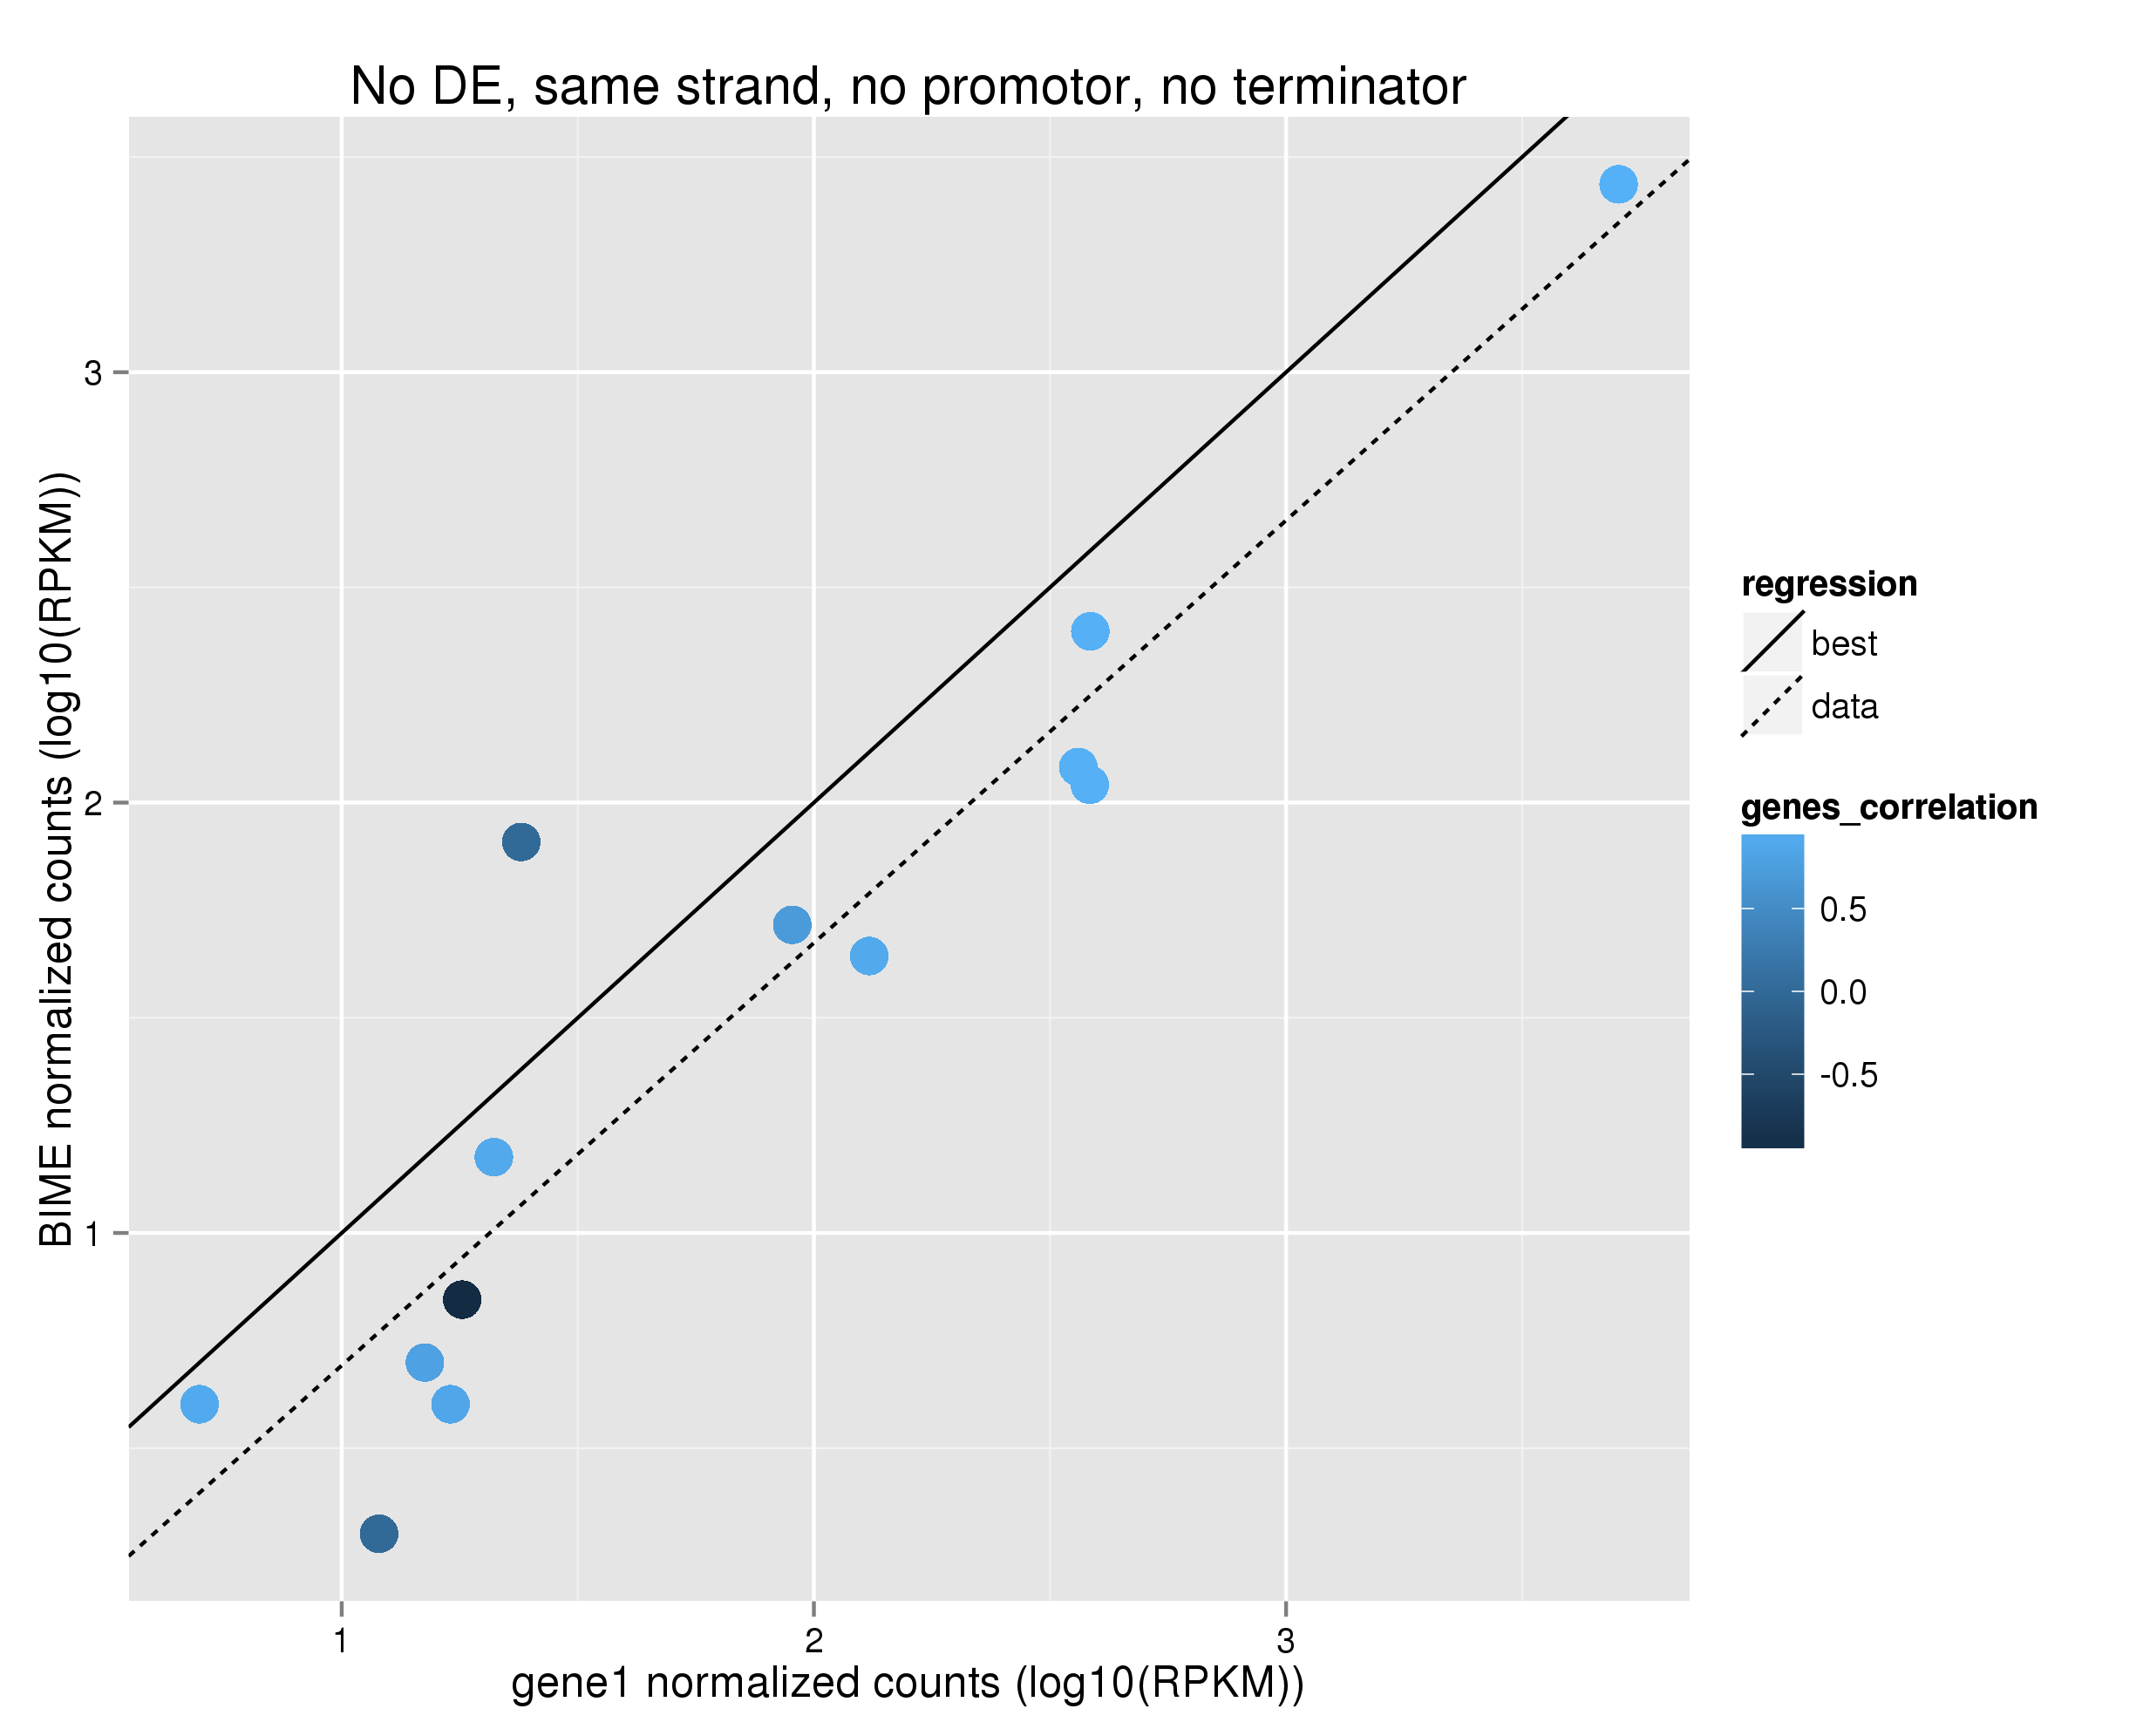
\includegraphics[scale=0.5]{figures/scatterplotSameStrandNoReg_all.png}
\caption{\textbf{Niveau d'expression de la BIME par rapport aux gènes flanquant non DE dans les opérons en absence de promoteurs et de terminateurs de transcription.} Les 3 jeux de données sont représentés ici. L'axe des abscisses représente le niveau d'expression du gène 1 en $log_{10}$, celui des ordonnées le niveau d'expression de la BIME en $log_{10}$. La coloration des points représente la corrélation du niveau d'expression du premier gène par rapport au second gène flanquant la BIME. La droite pleine représente la régression dans le cas où l'on observe une régression linéaire idéale, celle en pointillés représente la régression sur les valeurs des 3 jeux de données.
\label{fig:same_expression_operon_point}}}
\end{SCfigure}

Nous notons que la régression sur nos données tend vers une expression plus importante du premier gène par rapport à la BIME alors que nous nous attendions à trouver un même niveau d'expression pour la BIME et les deux gènes dans l'opéron pour des gènes dont le test de Wilcoxon n'est pas significatif. Nous pouvons donc penser qu'un biais de séquençage est bien présent pour les BIME, tendant vers une sous-expression de ces dernières. Afin de poursuivre l'étude de leur effet sur la transcription, nous étudierons leur impact de façon indirecte en nous intéressant aux niveaux d'expression des gènes flanquant les BIME.

\subsection*{Étude de l'expression des gènes dans les opérons}
Chez \textit{E. coli K12}, 1792 opérons sont formés d'un seul gène et sur les 848 autres opérons formés par plus d'un gène, 36 contiennent au moins une BIME et parmi ceux-ci 39 BIME sont répertoriées. Pour information, nous avons étudié la répartition de la composition en nombre de gènes de cette catégorisation et nous avons visualisé laquelle contient le plus de BIME (Figure \autoref{fig:operonFigA}).

\begin{figure}[h!]
\centering
\subfigure[]{\label{fig:operonFigA} 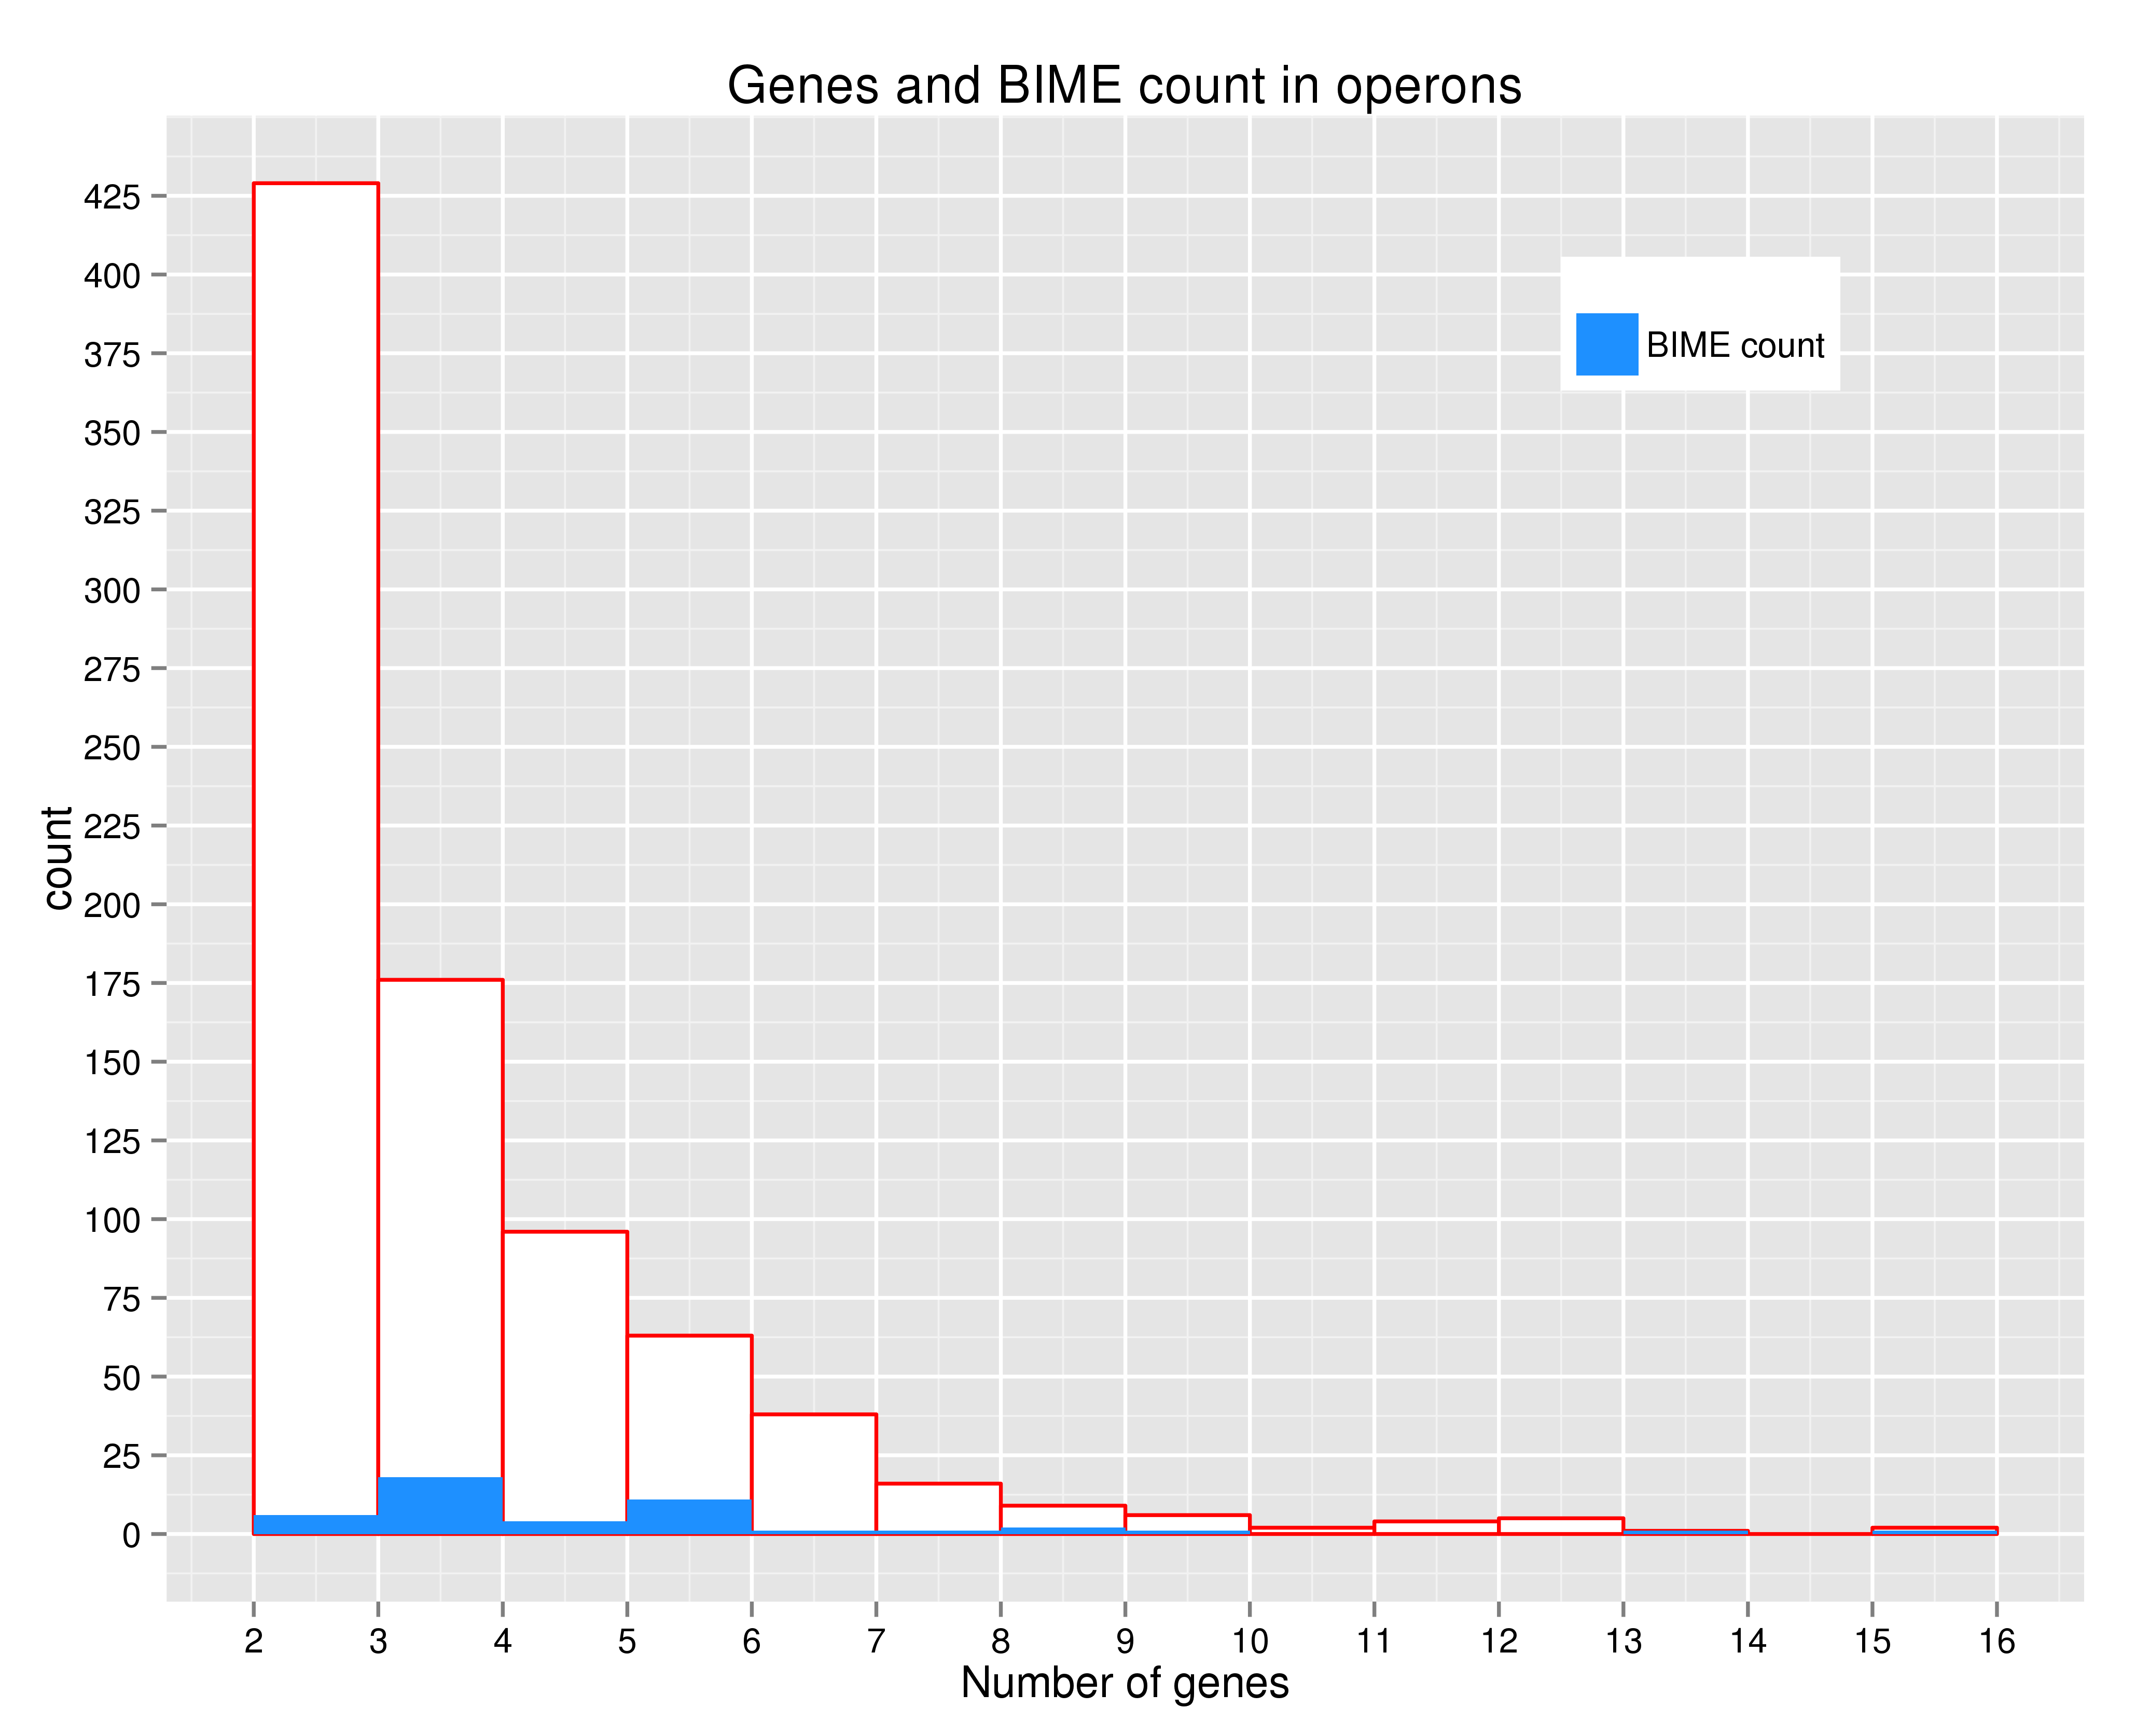
\includegraphics[scale=0.38]{figures/nbGenesBimeByOperon.png}}
\subfigure[]{\label{fig:operonFigB} 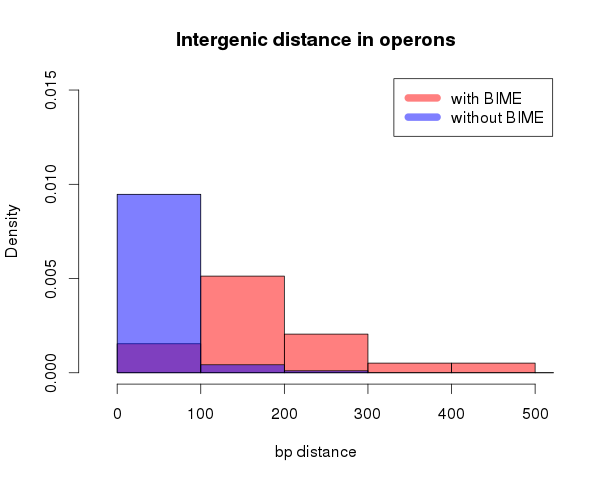
\includegraphics[scale=0.38]{figures/igr_distance.png}}
\subfigure[]{\label{fig:operonFigC} 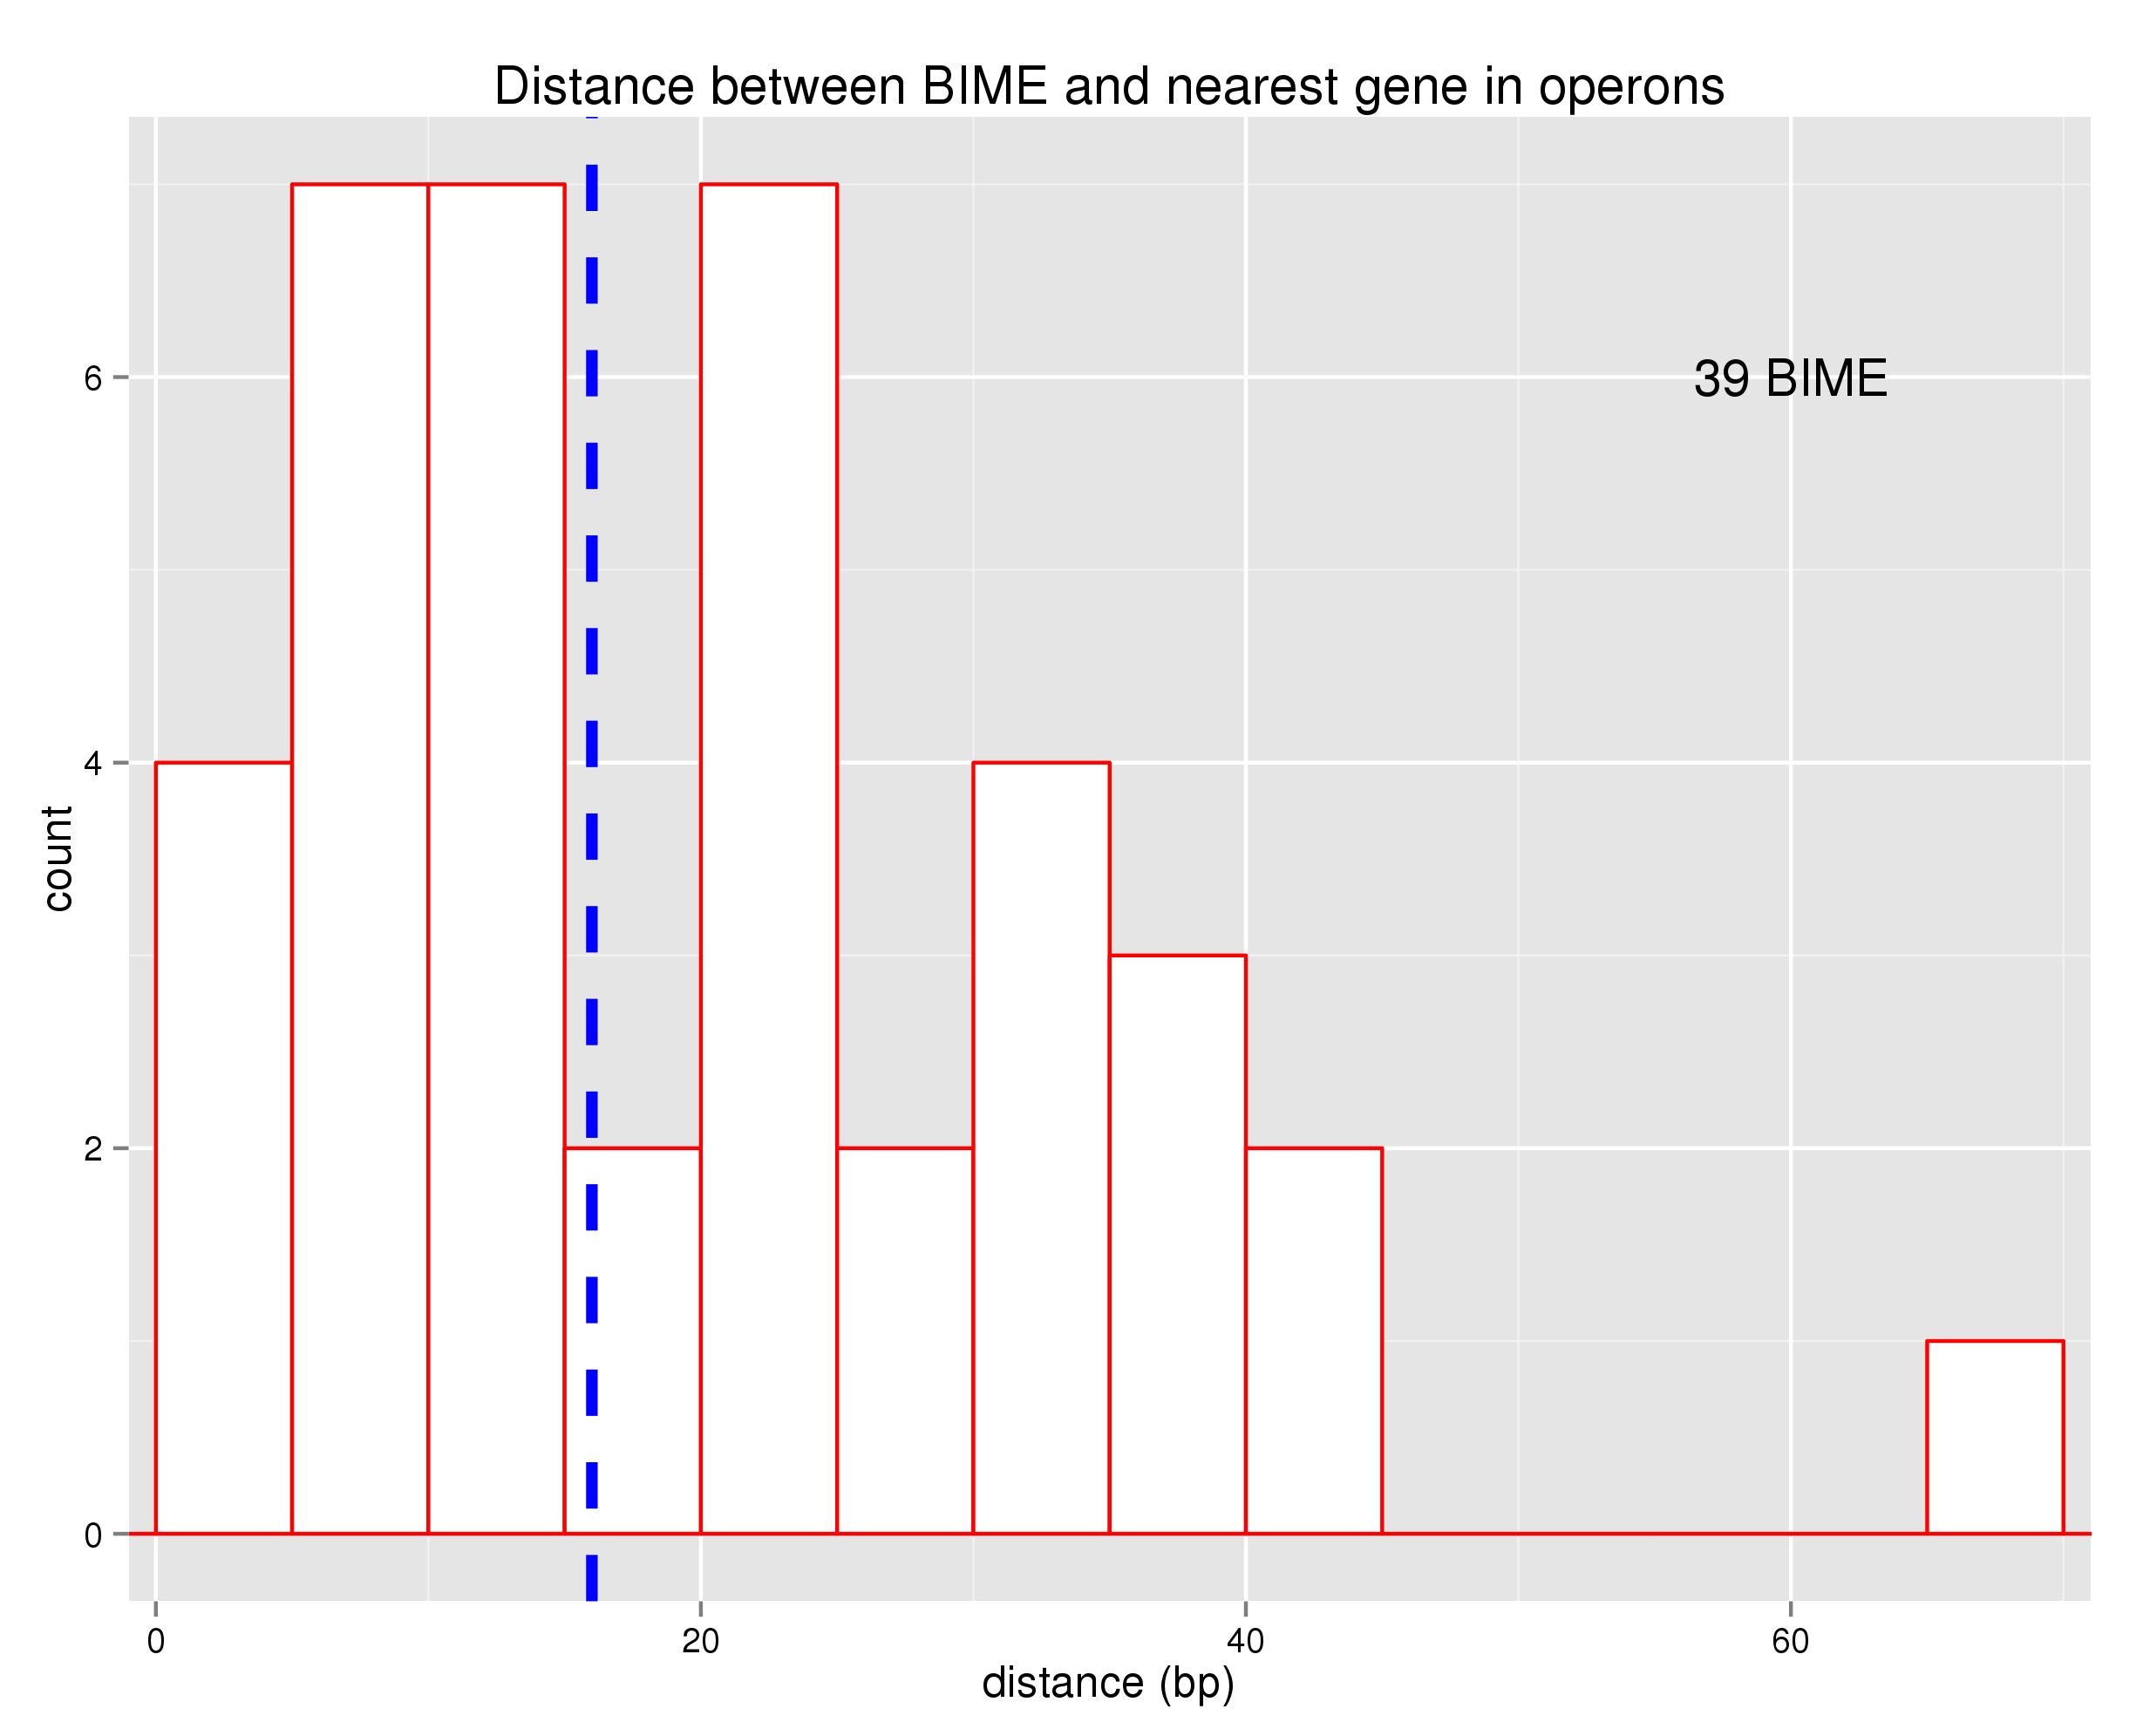
\includegraphics[scale=0.38]{figures/distance_BIME_gene_in_operon.png}}
\caption{\textbf{(a) Distribution du nombre de gènes par opérons et répartition des BIME.} L'échelle des abscisses indique le nombre de gènes dans l'opéron. Les histogrammes blancs représentent le compte du nombre d'opérons, les histogrammes bleus le compte des BIME au sein des opérons. La grande majorité des opérons sont constitués de 2 gènes mais peuvent aller jusqu'à 16 gènes. Sur les 36 BIME présentes dans les opérons, 18 sont dans des opérons de 3 gènes, 11 dans ceux de 5 gènes et 6 dans ceux de 2 gènes. \textbf{(b) Distances inter-géniques dans les opérons avec et sans BIME.} L'échelle des ordonnées représente la densité car l'écart entre les valeurs avec ou sans BIME est trop important pour une visualisation correcte de l'histogramme avec les comptes. En bleu absence de BIME dans la RIG, en rouge présence de BIME. Pour les données en absence de BIME, nous observons une valeur modale dans les régions inter-géniques de 50 pb, alors qu'en présence de BIME, la valeur modale se situe dans les régions inter-géniques de 150 pb. \textbf{(c) Distance de la BIME au gène le plus proche dans les opérons.} En abscisses le nombre de BIME, en ordonnées la distance de la BIME au gène le plus proche pour les 39 BIME situées dans les opérons. La ligne pointillé bleue représente la médiane des distances située à 16 pb.
\label{fig:operon}}
\end{figure}

Nous avons ensuite établi un indice d'expression, $I_{expr}$, permettant de mesurer l'écart entre le niveau d'expression de deux gènes consécutifs dans un opéron. La numérotation des gènes se faisant dans le sens de la transcription :
\[ I_{expr} = (gene2 - gene1) / (gene2 + gene1) \quad I_{expr} \in [-1,1]\]
Cet indice $I_{expr}$ permet de comparer la variation entre les couples de gènes quelque soit leur niveau d'expression. Si le premier gène est plus exprimé que le second, la valeur de $I_{expr}$ est négative sinon elle devient positive. Cet indice nous a permis de nous intéresser aux niveaux d'expression des gènes des opérons en observant trois facteurs de la \gls{rig}, la présence d'une BIME, la présence de promoteurs et/ou de terminateurs de transcription et la taille de cette région. Les annotations des promoteurs et des terminateurs proviennent respectivement de RegulonDB et Door\up{2}DB et sont issus à la fois de validations expérimentales et de prédictions. Nous avons fait le choix de ne pas distinguer les cas de présence seule d'un promoteur, ou d'un terminateur et avons rassemblé ces catégorie sous l'intitulé promoteur/terminateur pour ne pas tomber dans des cas où nous aurions trop peu de données, surtout en présence de BIME, et pour diminuer le nombre de catégories à traiter. En effet, au lieu d'une catégorie nous aurions trois catégories (promoteur seul, terminateur seul et promoteur avec terminateur) ce qui limiterait la compréhension de la représentation graphique. Pour la taille de la RIG, nous avons étudié la distance inter-génique dans les opérons en présence ou absence de BIME (Figure \autoref{fig:operonFigB}). La taille des RIG ne contenant pas de BIME possède une valeur modale de 50 pb alors qu'en leur absence celle-ci se situe à 150 pb. Nous avons fixé le seuil de la taille de la RIG à 150 pb.

\begin{figure}[!h]
\centerline{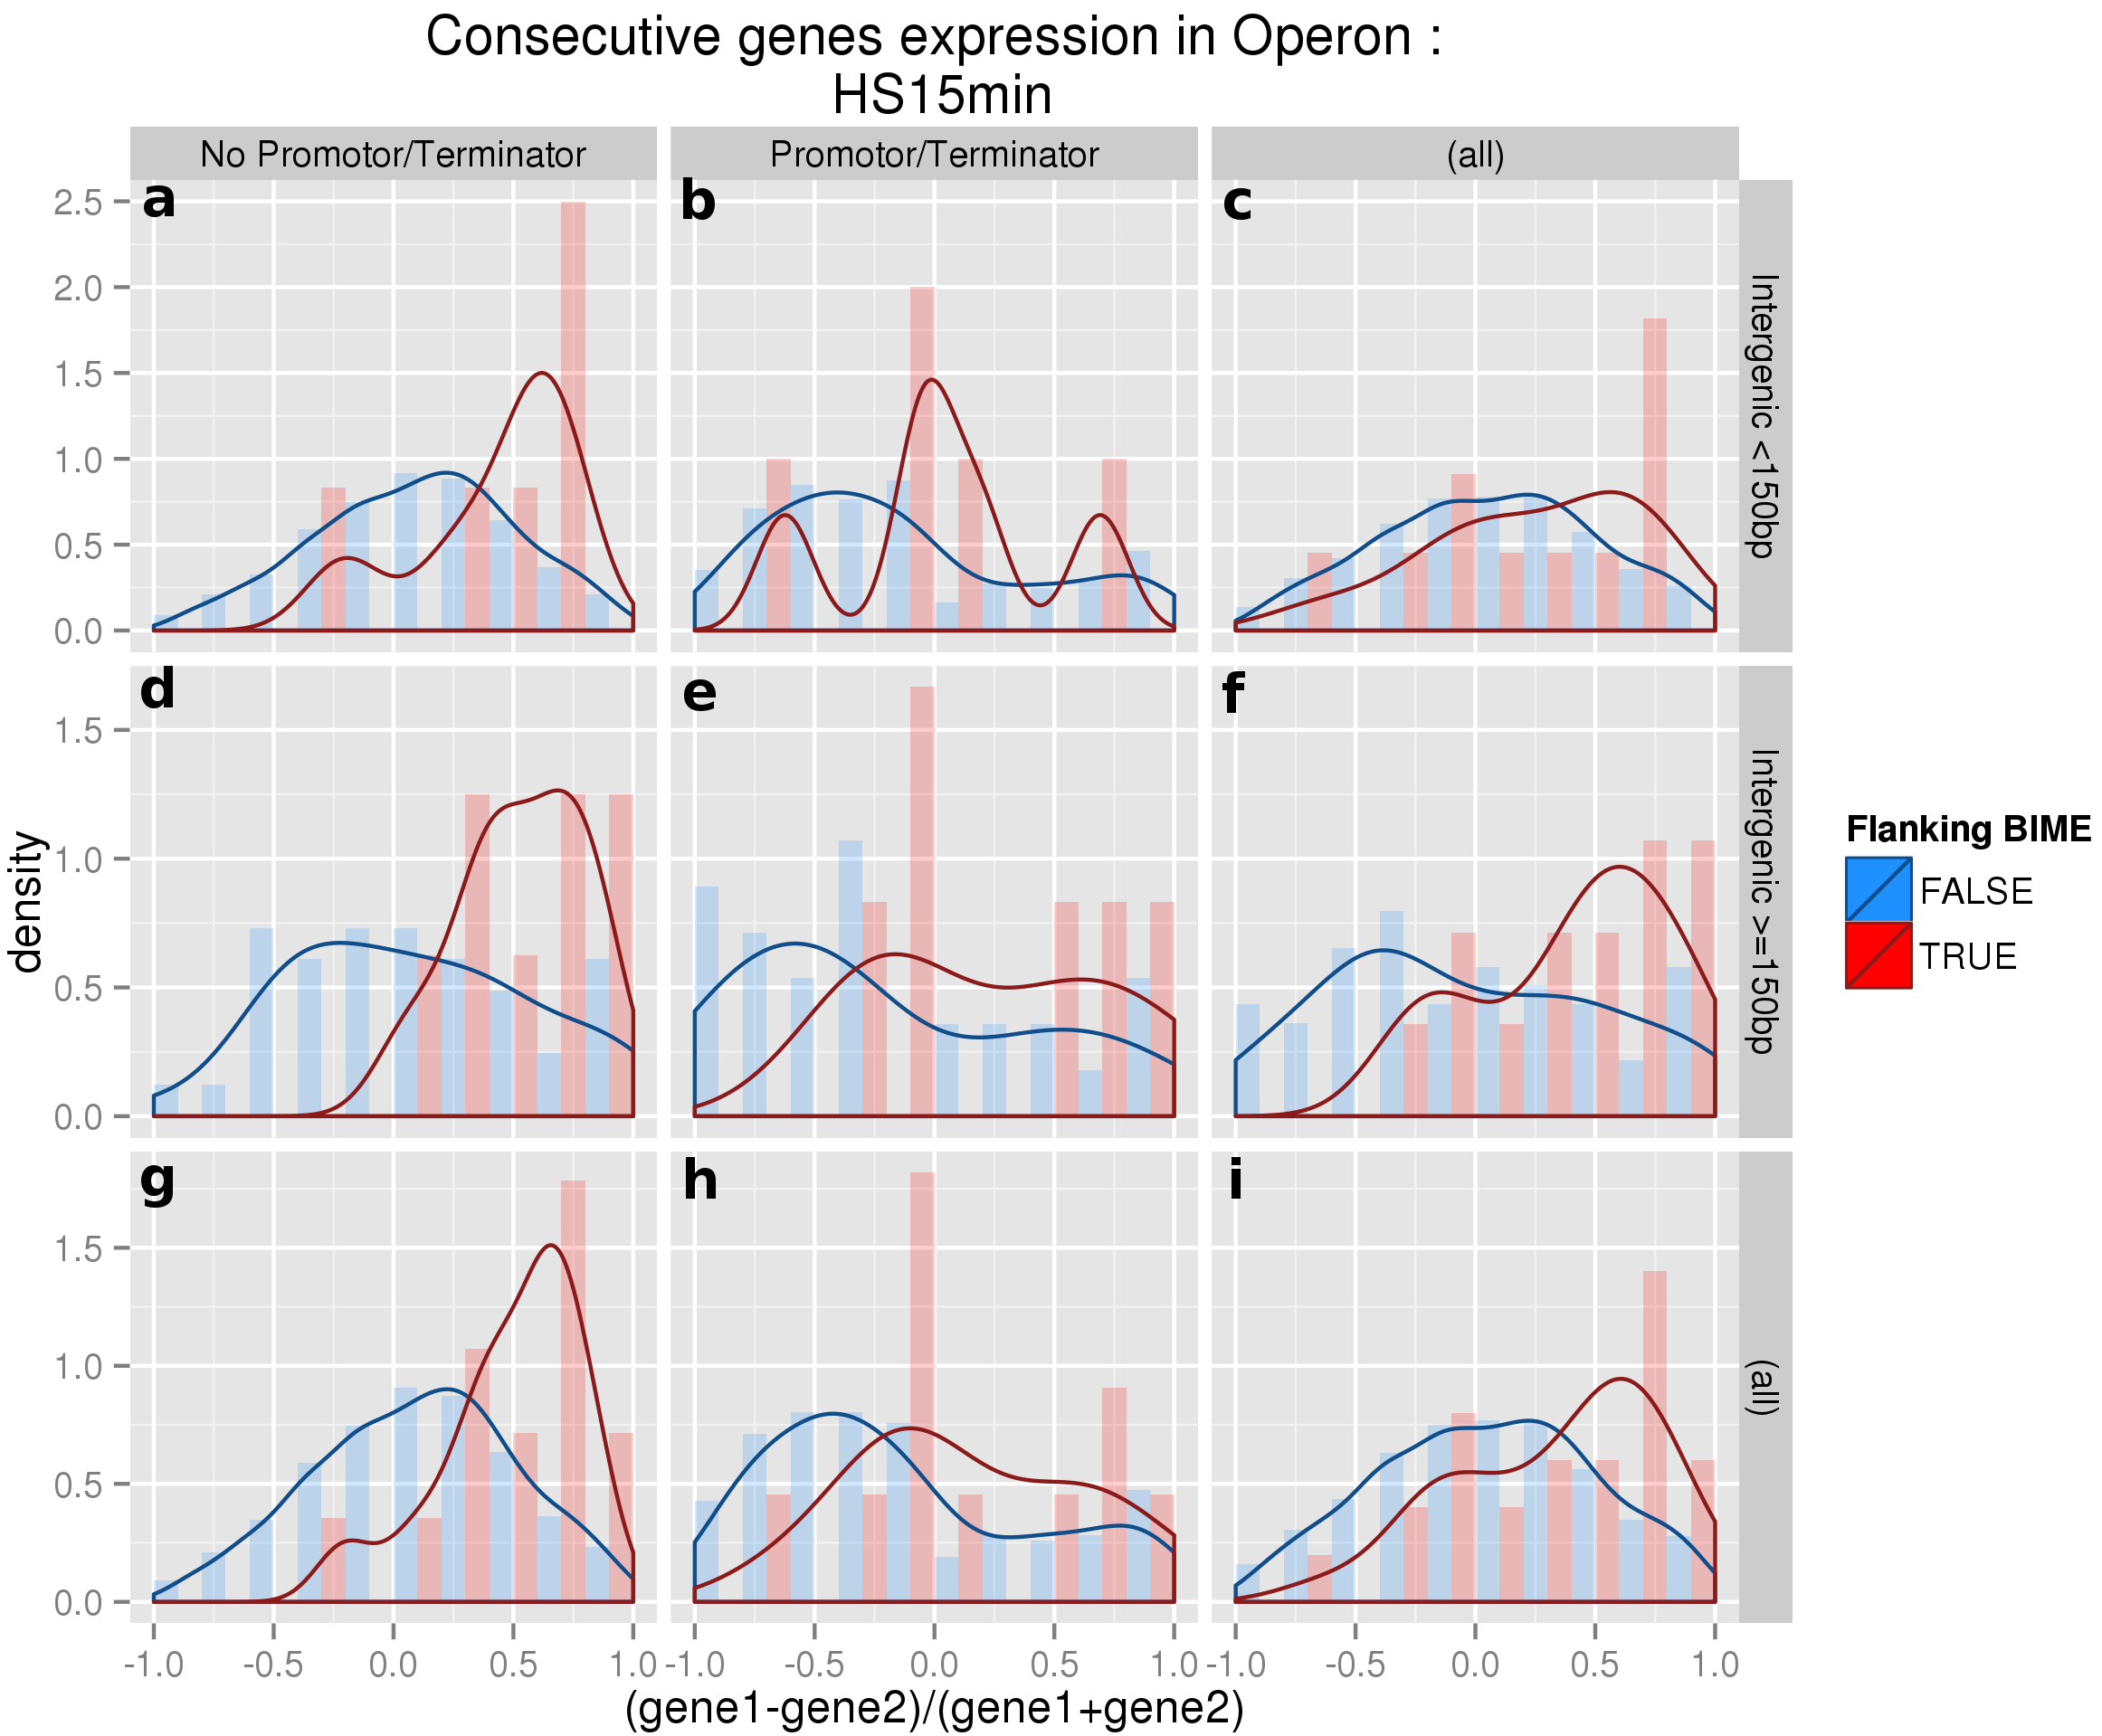
\includegraphics[scale=0.82]{figures/genesOperon_histoDens.png}}
\caption{\textbf{Niveau d'expression des gènes consécutifs dans les opérons.} Les données proviennent de l'expérience de choc thermique pendant 15 minutes (HS-15min). L'$I_{expr}$ en abscisses est l'indice d'expression du gène 1 par rapport au gène 2 $(gene2 - gene1) / (gene2 + gene1)$, borné sur [-1,1]. Les valeurs négatives indiquent un niveau d'expression plus élevé du gène 1, les valeurs positives l'inverse. Les éléments de couleur rouge se réfèrent aux gènes flanquant une BIME, ceux en bleu aux gènes sans BIME entre eux. Les histogrammes indiquent la densité pour chacune des valeurs de l'$I_{expr}$. Les courbes de densité montrent la tendance de l'$I_{expr}$ par rapport à la présence/absence de BIME, la comparaison entre les 2 distributions est réalisée à l'aide d'un test de Wilcoxon dont la p-valeur est affichée dans chaque graphique. Les graphiques sont décomposées sur 2 critères, les \gls{et} dans la RIG et la taille de la RIG (<150 pb ou >= 150 pb).}
\label{fig:expression_operon}
\end{figure}

L'analyse menée sur les données d'expression des bactéries soumises à un choc thermique pendant 15 minutes (HS-15min) est représentative des deux autres jeux de données (Voir annexe \ref{annexeOperon}). La comparaison des distributions en présence et absence de BIME est effectuée à l'aide d'un test de Wilcoxon (p-valeur significative < 0.05) car toutes les distributions ne suivent pas une loi normale (test de Shapiro), l'hypothèse nulle étant la similitude des distributions. L'absence de BIME montre une répartition symétrique de l'expression des deux gènes centrée sur une valeur d'$I_{expr}$ à zéro sauf en présence de promoteurs/terminateurs dans la RIG, la tendance étant vers une expression plus importante du gène 2 (\autoref{fig:expression_operon} - (b,e,h)).
En s'intéressant dans un premier temps au RIG de moins de 150 pb, en présence de promoteur/terminateur, le test statistique ne montre pas de différence entre les deux distributions (\autoref{fig:expression_operon} - (b); p-valeur: 0.216), ce qui n'est pas le cas en leur absence ou avec toutes les valeurs (\autoref{fig:expression_operon} - (a-c); p-valeurs: 0.024, 0.032). 
Pour les RIG de plus de 150 pb, la tendance vers un niveau d'expression supérieur du gène 1 est plus marquée avec un décalage de la courbe en présence de BIME (rouge) vers la gauche mais la significativité n'est pas avérée sauf lorsque le facteur promoteur/terminateur n'est plus pris en compte  (\autoref{fig:expression_operon} - (f); p-valeur: 0.022). 
En étudiant maintenant le facteur promoteur/terminateur, nous remarquons en leur absence une tendance à l'expression plus importante du gène 1 qui devient significative en ne s'intéressant plus à la taille de la RIG (\autoref{fig:expression_operon} - (g); p-valeur: 0.0006). En leur présence, nous notons que la courbe marquant l'absence de BIME (bleue) tend vers les valeurs positives, donc une expression plus importante du gène 2, ceci s'explique par la présence de promoteurs dans la RIG (\autoref{fig:expression_operon} - (b,e,h); p-valeurs: 0.216, 0.057, 0.028). Le décalage de la courbe des BIME (rouge) vers les valeurs négatives est visible de façon plus ou moins marquée dans tous les cas de figure, cet effet est peut être dû à rôle de terminateur de transcription joué par les BIME ou à un effet de stabilisation de la partie 5' du transcrit favorisé par la présence de la BIME.

En approfondissant l'étude de ses données et en nous plaçant dans le cas de la (\autoref{fig:expression_operon} - (i)), nous nous intéressons à la distribution de l'$I_{expr}$ en n'ayant que pour critère la présence ou l'absence de BIME et la relation existant entre l'absence d'ET et la présence de chacun d'entre eux. En étudiant d'abord les cas en absence de BIME (\autoref{fig:expression_operon_reg}-(a)), nous observons un effet des promoteurs avec une expression plus importante du gène 2 (courbe verte) et l'effet inverse pour la courbe des terminateurs de transcription (courbe orange). Ces deux effets sont visibles de façon plus modérée sur la courbe des promoteurs et terminateurs (courbe violette). Quand à la courbe des RIG sans ET, elle est symétrique et centrée sur sur une valeur négative mais proche de zéro. Des tests de Wilcoxon ont été réalisés entre les valeurs d'$I_{expr}$ sans ET (courbes bleues) dans la RIG et chacun des trois autres cas de figure (\autoref{table:p-val_reg}). Ces résultats nous indiquent qu'il existe une différence significative entre la distribution sans ET et les trois autres (p-valeurs < 0.05), résultat attendu puisque les ET ont un effet sur la transcription des gènes. En revanche dans le cas où les BIME sont présentes (\autoref{fig:expression_operon_reg}-(b)), uniquement la distribution de l'$I_{expr}$ contenant des promoteurs se différencie de manière significative (p-valeurs : 0.034) de celle sans ET, visible également sur le graphique avec un décalage de toutes les courbes vers une expression plus importante du premier gène. Ce résultat nous conforte dans l'hypothèse que les BIME joueraient un rôle similaire aux terminateurs de transcription ou de stabilisation de la partie 5' du transcrit face au dégradosome.

\begin{SCfigure}[][h!]
\fbox{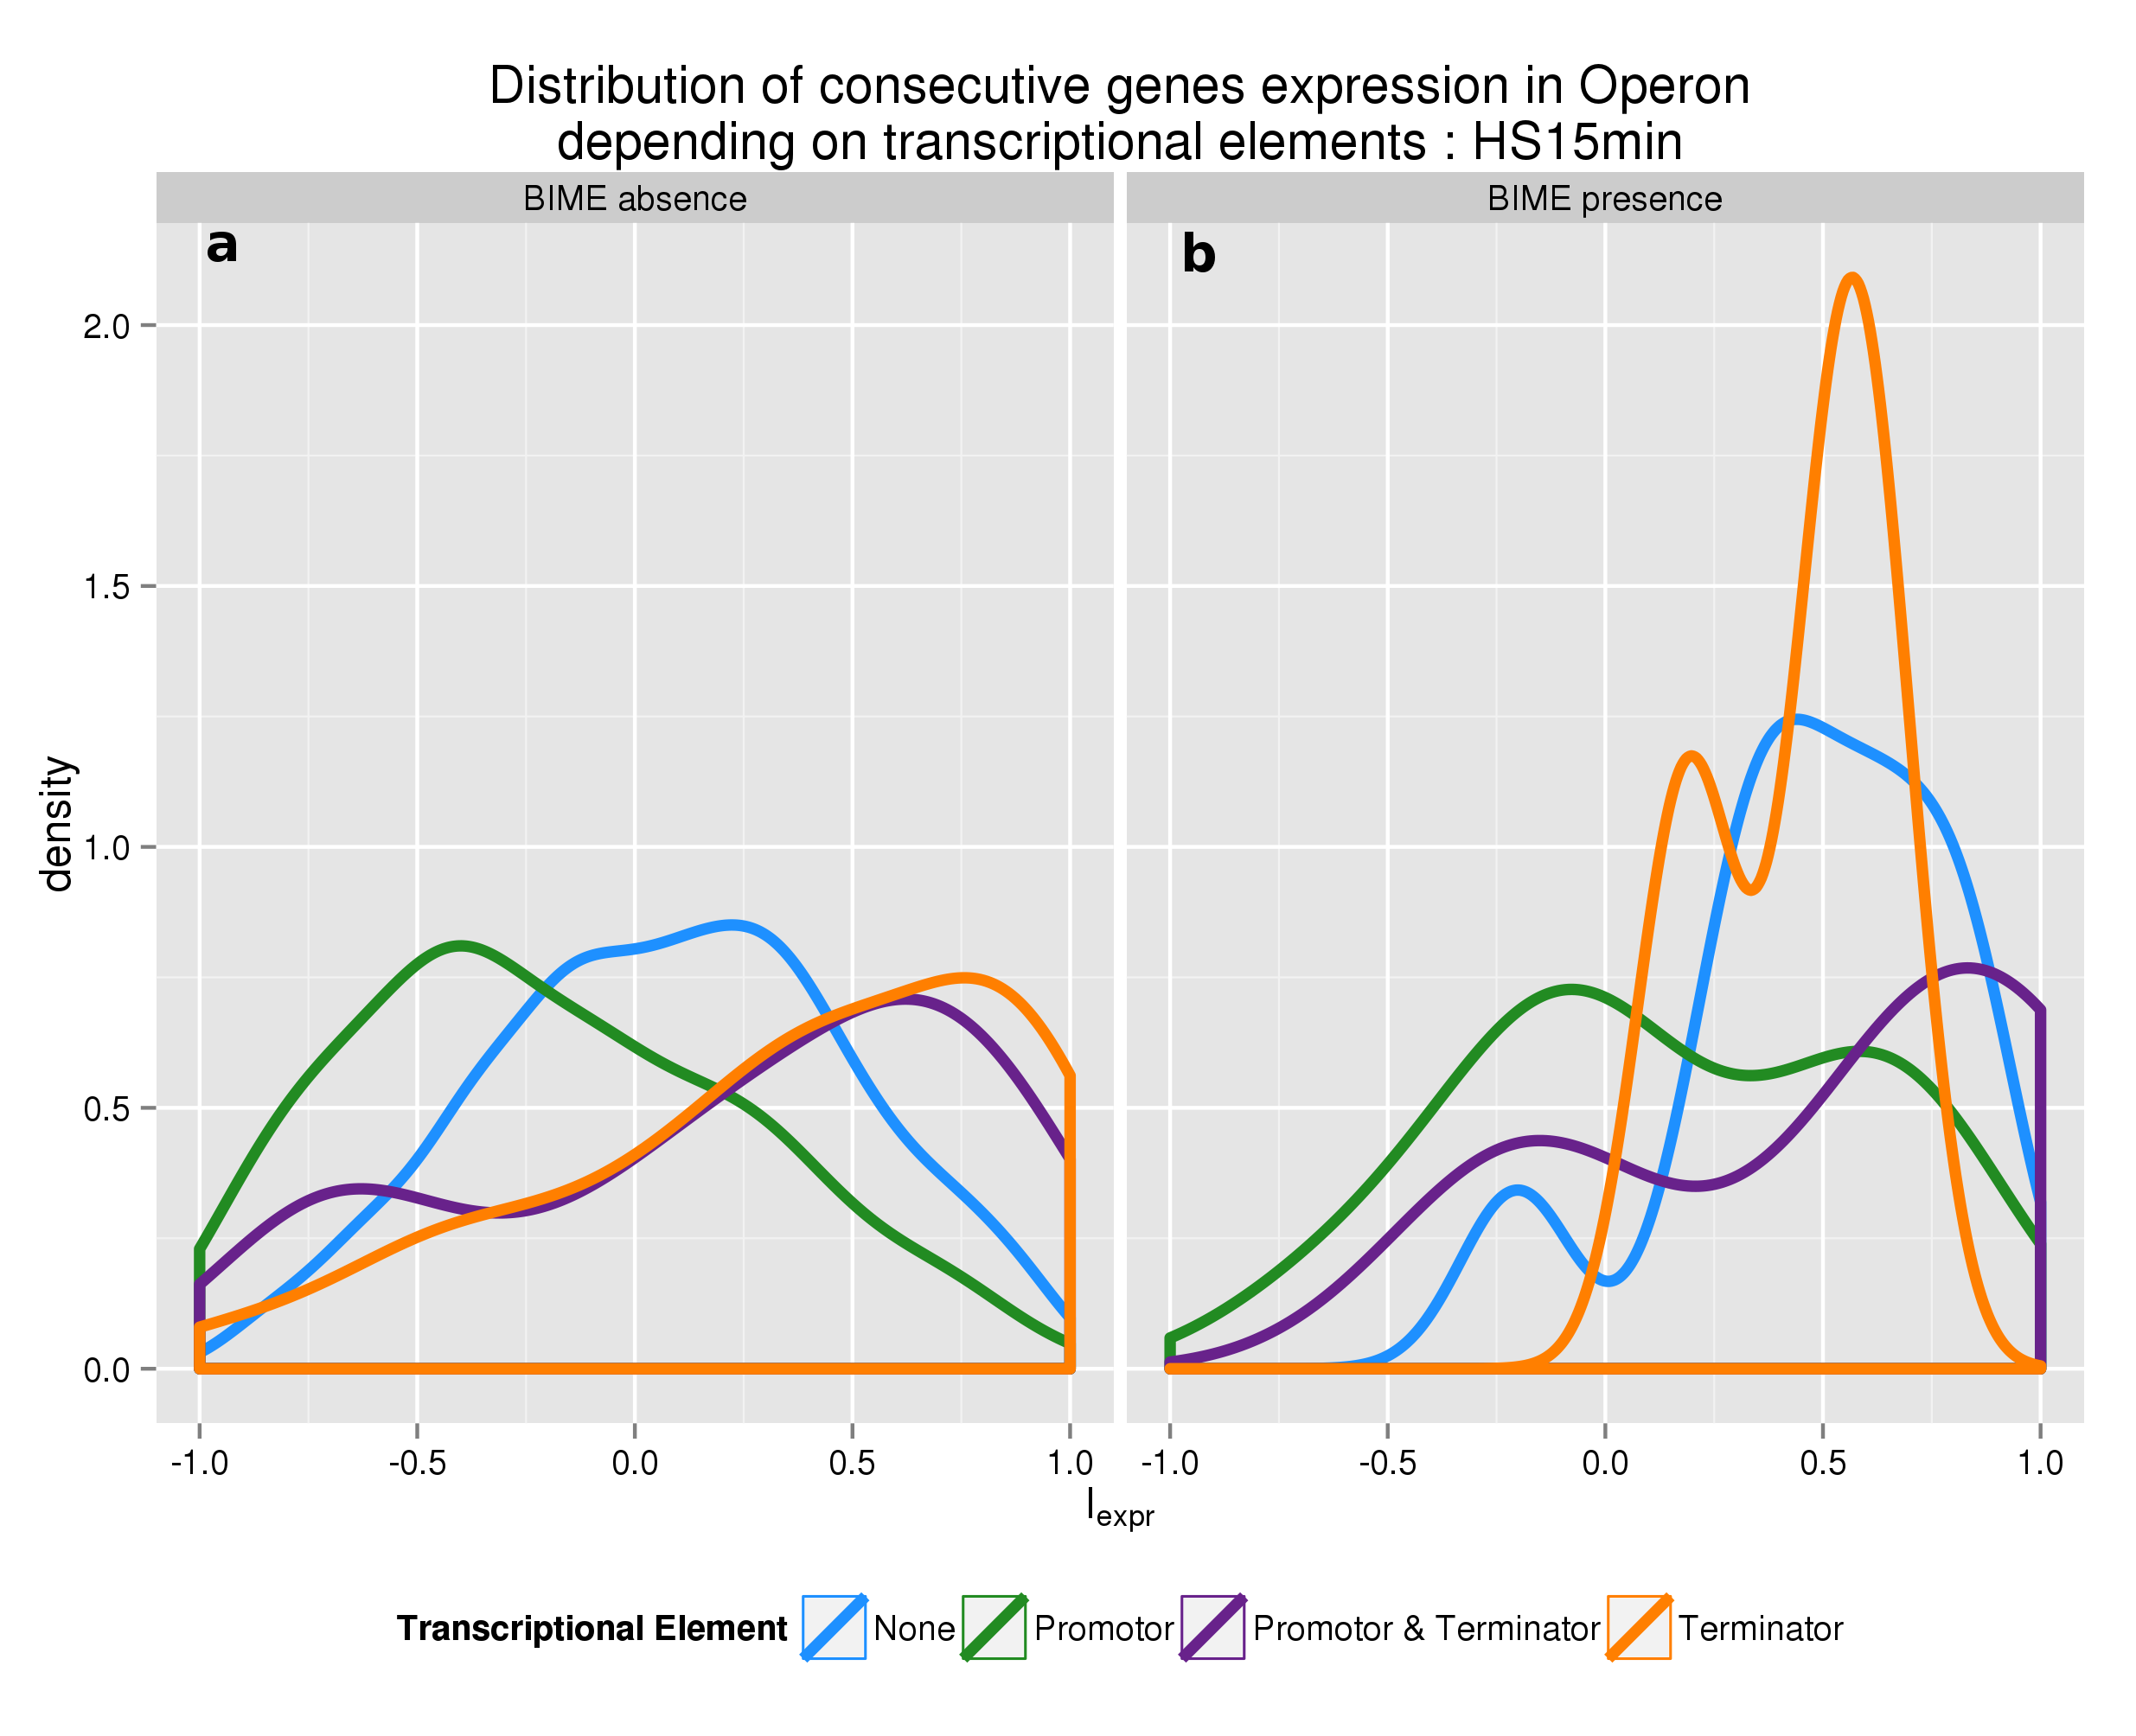
\includegraphics[scale=0.5]{figures/genesOperonReg_histoDens.png}
\caption{\textbf{Niveau d'expression des gènes consécutifs dans les opérons en fonction des éléments transcriptionnels (ET).} L'$I_{expr}$ en abscisses est l'indice d'expression du gène 1 par rapport au gène 2 $(gene2 - gene1) / (gene2 + gene1)$, borné sur [-1,1]. Les valeurs négatives indiquent un niveau d'expression plus élevé du gène 1, les valeurs positives l'inverse. Les courbes de densité indiquent la distribution de l'$I_{expr}$ en fonction des ET présent dans la RIG. Les courbes bleues indiquent l'absence de promoteur et/ou de terminateur de transcription, les vertes la présence de promoteur uniquement, les oranges la présence de terminateurs de transcription uniquement et les violettes la présence à la fois de promoteurs et de terminateurs transcription. \textbf{(a)} présence de BIME dans la RIG, \textbf{(b)} absence de BIME dans la RIG.
\label{fig:expression_operon_reg}}}
\end{SCfigure}

\begin{table}[h!]
\centerline{
\begin{tabular}{|l|c|c|c|}
  \hline
  \multirow{2}{*}{Wilcoxon test p-valeurs} & \multicolumn{3}{|c|}{\cellcolor{Gray}Élément transcriptionnel} \\
  \cline{2-4}
  & \cellcolor{Gray}Promoteur & \cellcolor{Gray}Terminateur & Promoteur \& \cellcolor{Gray}Terminateur\\  
  \hline
  Absence de BIME & $5.48~e^{-14}$ & $7.3~e^{-5}$ & $0.0091$ \\ 
  \hline
  Présence de BIME & $0.034$ & $0.375$ & $0.921$ \\
 \hline
\end{tabular}}
\caption{\textbf{P-valeurs des tests de Wilcoxon des $I_{expr}$ en présence des éléments transcriptionnels comparé à leur absence.} Les p-valeurs sont présentées en présence et en absence de BIME et renvoient aux cas de la \autoref{fig:expression_operon_reg}-(i).
\label{table:p-val_reg}}
\end{table}

Afin d'approfondir ces hypothèses, nous avons étudié plus en détail le niveau d'expression des gènes dans les 36 opérons contenant des BIME.

\section*{Étude des opérons, différence d'expression en présence de BIME}
\label{expression_operon}
L'hypothèse privilégiée ici est que les gènes appartenant à un opéron vont être exprimés à un niveau similaire, la question qui se pose est de savoir si la présence d'une BIME entre deux gènes d'un opéron va avoir un impact sur la transcription ou la dégradation d'un des gènes. Dans ce cadre, les opérons contenant des BIME sont sélectionnés et l'expression des deux gènes de l'opéron flanquant la BIME prise en compte si au moins un des deux gènes a une couverture > 10, cette valeur est choisie car elle représente le premier quartile de nos données, supprimant les gènes les moins exprimés. De plus, cela nous permet d'éliminer des variations qui seraient jugées importantes pour de petites valeurs (e.g: 2 et 8 qui implique un facteur 4 pour le changement d'expression). Nous avons vérifié par un test de Shapiro que nos valeurs de comptage ne suivaient pas une loi Normale, ce qui nous a conduit à choisir d'appliquer un test non paramétrique de rangs de Wilcoxon si l'expérience contient au moins 5 réplicats et un test de Student si l'expérience contient moins de réplicats. L'hypothèse nulle de ces tests est qu'il n'existe pas de DE entre les 2 gènes. La p-valeur significative étant fixée à 0.01 pour nous permettre d'être plus stricts sans pour autant limiter les résultats. Nous n'avons pas jugé utile d'appliquer de correction à ces tests car le nombre d'opérons contenant des BIME se limite à 36.

Pour les gènes dont le test est significatif, deux représentations graphiques sont générées. La 1\up{ère} est un schéma décrivant les niveaux d'expression normalisé des gènes de l'opéron ainsi que la position relative des REP formant la BIME (Figure \autoref{fig:expressionFigA}). La 2\up{nde} est une représentation de la couverture sur l'opéron par rapport à l'organisation génomique de celui-ci ainsi que la catégorisation des REP composant la BIME (Figure \autoref{fig:expressionFigB}).

\begin{figure}[h]
\centering
\subfigure[]{\label{fig:expressionFigA} 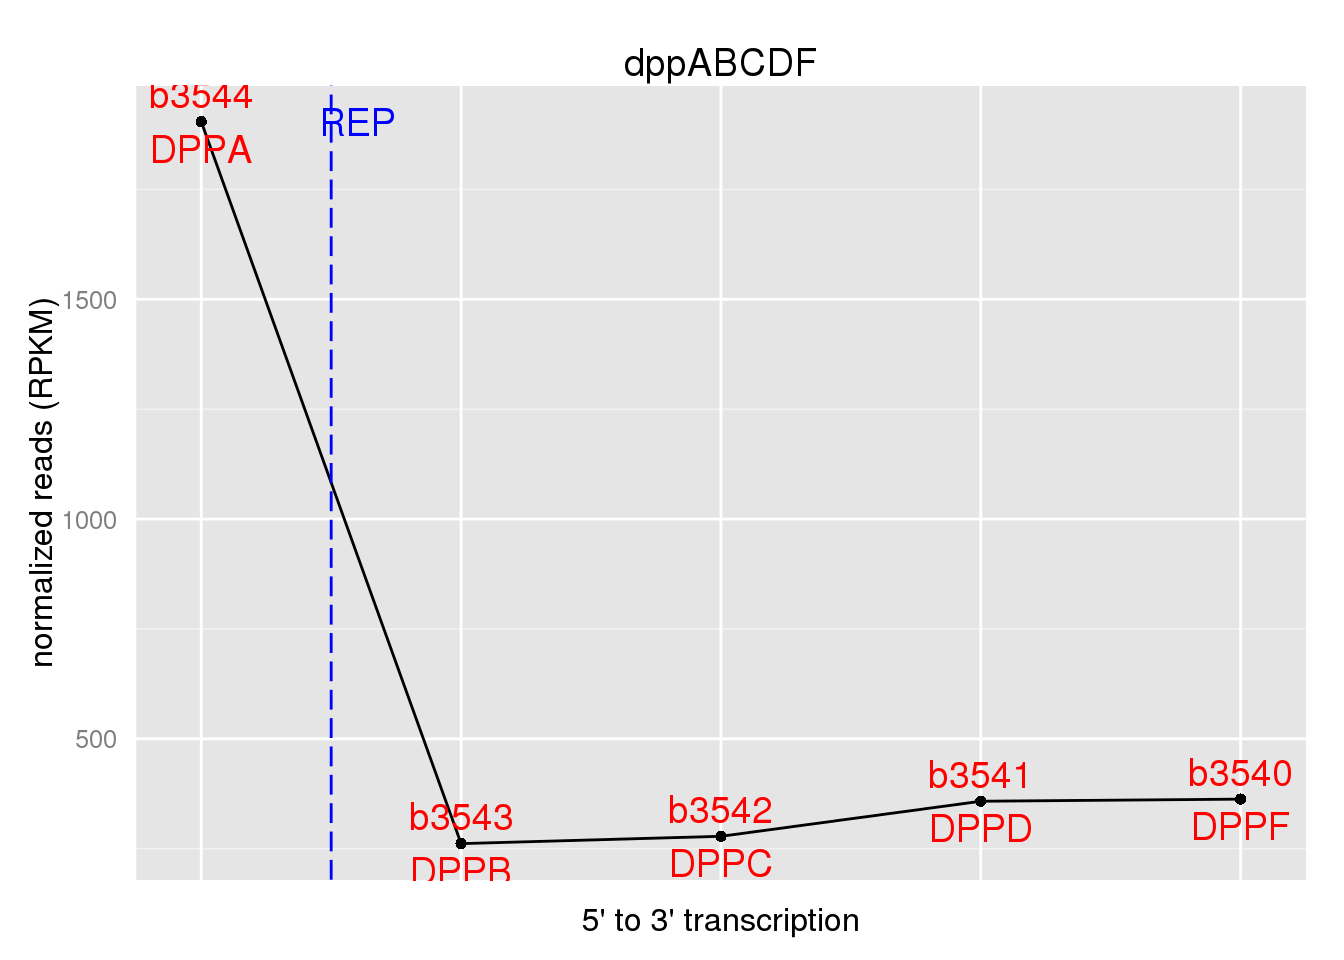
\includegraphics[scale=0.35]{figures/expression1.png}}
\subfigure[]{\label{fig:expressionFigB} 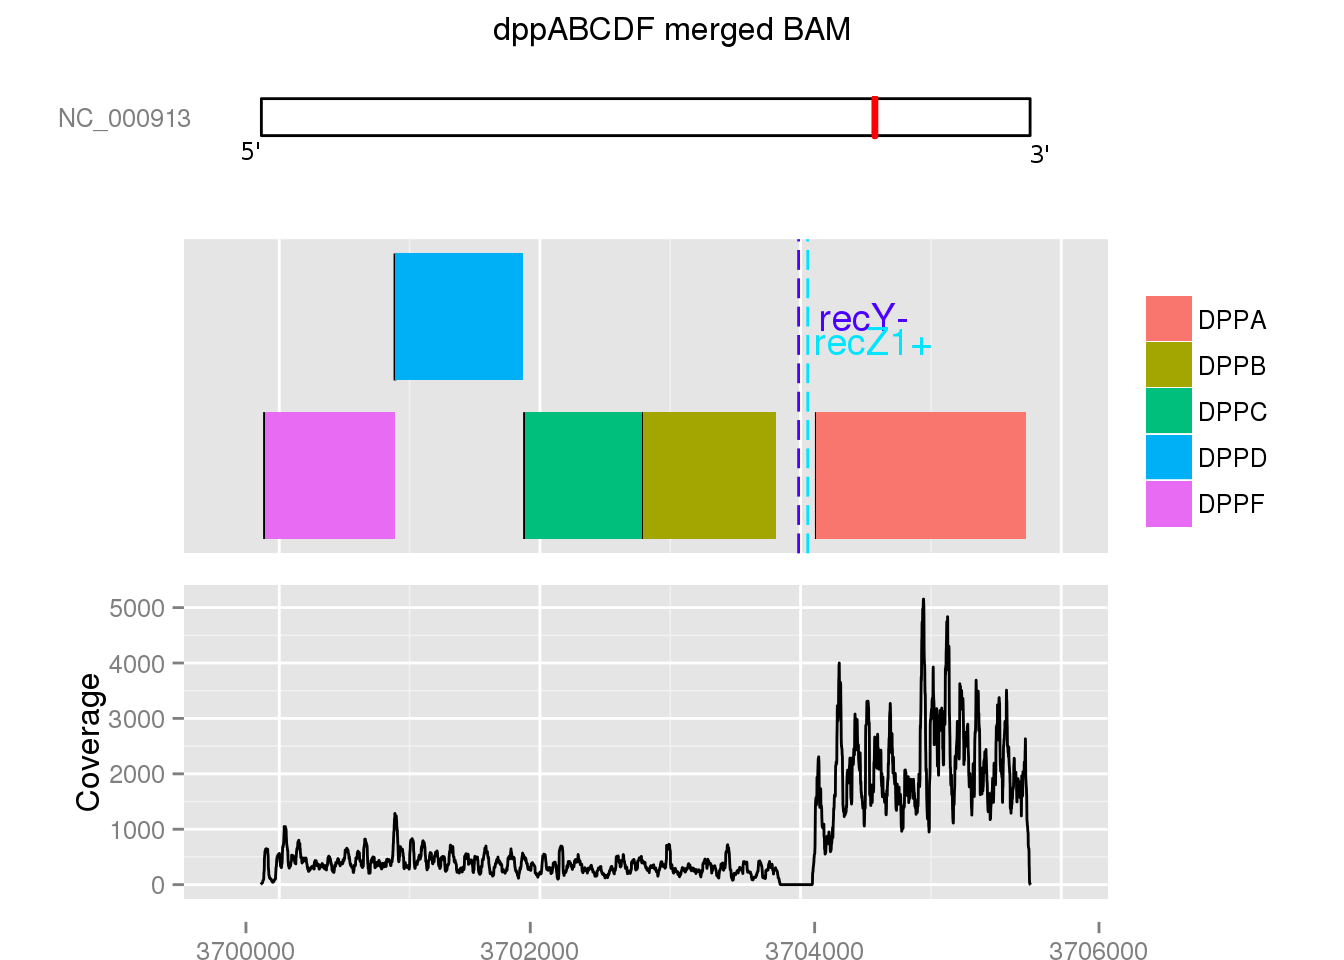
\includegraphics[scale=0.35]{figures/expression2.png}}
\caption{\textbf{Résultats de l'étude de l'expression des gènes dans les opérons contenant des BIME. (a)} Le taux d'expression normalisé de chaque gène de l'opéron est représenté en ordonnées, l'organisation des gènes de l'opéron est schématisée sur l'axe des abscisses dans le sens 5' $\mapsto$ 3', l'orientation du brin est notée sur l'axe des abscisses. La position de la ou les REP composant la BIME est schématisée par la ligne bleue verticale. En tenant compte de l'orientation du brin, si au moins un promoteur ou un terminateur de transcription est présent dans la RIG contenant la BIME, ceux-ci sont représentés respectivement par une ligne en pointillés verticale verte ou rouge. \textbf{(b)} La position de l'opéron sur le génome est indiquée par la barre rouge sur l'idéogramme de la partie supérieure. La partie médiane représente l'organisation des gènes de l'opéron dans le sens 5' $\mapsto$ 3' (le sens du brin est précisé dans le titre) ainsi que le positionnement et la classe des REP composant la BIME. La partie inférieure montre la couverture issue des fichiers BAM fusionnés de l'expérience par rapport à l'organisation de la partie médiane.}
\label{fig:expression} 
\end{figure}

Nous avons testé cette méthode sur nos trois jeux de données qui ont produit les résultats du \autoref{table:expression}.

\begin{table}[h!]
\centerline{
\begin{tabular}{|l|c|c|c|c|}
  \hline
  \rowcolor{Gray} Jeux de données & $\frac{Nb.~operons~avec~genes~DE}{Nb.~d'operons~exprimes}$ & \begin{tabular}{c}Nb. de\\BIME\end{tabular} & \begin{tabular}{c}Nb. de RIG\\avec Terminateurs\end{tabular} & \begin{tabular}{c}Nb. de\\Transporteurs ABC\end{tabular}\\ 
  \hline
  GSE61327\_ALE & 17/32 & 18 & 7 & 7\\  
  \hline
  HS-15min & 8/20 & 8 & 1 & 4\\ 
  \hline
  M-P4h & 12/30 & 12 & 4 & 5 \\
 \hline
\end{tabular}}
\caption{\textbf{Résultats de l'étude de différence d'expression des gènes des opérons flanquant une BIME.} La 2\up{ème} colonne indique le nombre d'opérons contenant 2 gènes flanquant une BIME pour lesquels nous observons une différence de niveau d'expression sur le nombre d'opérons dont les 2 gènes flanquant la BIME sont exprimés (au moins un des 2 gènes possède une couverture > 10). La 3\up{ème} colonne indique le nombre de BIME concernées, un opéron pouvant en contenir plusieurs. La 4\up{ème}, le nombre d'opérons contenant un terminateur de transcription dans la RIG contenant également une BIME pour les gènes DE. La dernière colonne indique le nombre de transporteurs ABC parmi les opérons dont les gènes sont DE.
\label{table:expression}}
\end{table}

Sur les résultats obtenus, nous constatons tout d'abord une hétérogénéité du nombre d'opérons exprimés, ce phénomène n'est pas une surprise car les trois jeux de données sont issus de conditions de culture différentes donc de voies métaboliques distinctes. Concernant les terminateurs de transcription présent dans la RIG contenant la BIME, 2/7 se situent avant la BIME, 3/7 la chevauchent et 2/7 sont après pour GSE61327\_ALE. Le terminateur est situé après la BIME pour HS-15min. Pour M-P4h, un seul terminateur est situé avant la BIME, 2/4 la chevauchent et un seul est situé après. \textcolor{red}{Le phénomène de colocalisation des BIME et des terminateurs pourrait indiquer un rôle de la BIME dans la terminaison de transcription ou tout du moins d'atténuation dans les opérons car dans les six cas de chevauchement avec le terminateur, nous observons un niveau d'expression diminué du second gène par rapport au premier.}

\textcolor{red}{Rôle des transporteurs ABC à explorer et voir quelle partie du transporteur est plus exprimée}

\section*{Approche locale, corrélation de profils d'expression}
\label{approche_locale}
Nous avons développé une méthode réalisant un test de corrélation entre les profils d'expression des régions contenant des BIME et un profil modèle de changement d'expression en modifiant la technique mise au point pour la prédiction d'opérons dans les génomes bactériens \citep{Fortino2014} décrite dans la partie \nameref{methode_correlation}. Elle a été adaptée pour nous permettre de localiser le point de cassure dans la RIG contenant une BIME. Au lieu de faire une recherche sur le génome complet, nous avons privilégié une approche locale en ciblant des régions d'intérêt qu'il a fallu au préalable délimiter. Celles-ci se modélisent par la présence du 1\up{er} gène, de la 1\up{ère} RIG, de la BIME, de la 2\up{nde} RIG et du 2\up{nd} gène. Une fois ces régions extraites, le calcul de la couverture base par base a été réalisé à l'aide des BEDtools (Annexe \ref{annexeCodeCov}).



Les seuils que nous avons utilisés sont différents de ceux de la méthode originelle et nous avons introduit un filtre supplémentaire quand à la couverture minimale d'un des deux gènes : 
\begin{itemize}[label=$\bullet$]
\item fenêtre glissante de 300 bases
\item au moins un des deux gènes possède une couverture > 10
\item $log_2(\frac{\overline{couverture~droite}~+~1}{\overline{couverture~gauche}~+~1})~\geq~1$ pour un profil \_\_\_|\^{ }\^{ }\^{ }
\item $log_2(\frac{\overline{couverture~gauche}~+~1}{\overline{couverture~droite}~+~1})~\geq~1$ pour un profil \^{ }\^{ }\^{ }|\_\_\_
\item une corrélation > 0.5
\item une p-valeur du test de corrélation $< 10^{-7}$
\end{itemize}

\begin{figure}[!h]
\centerline{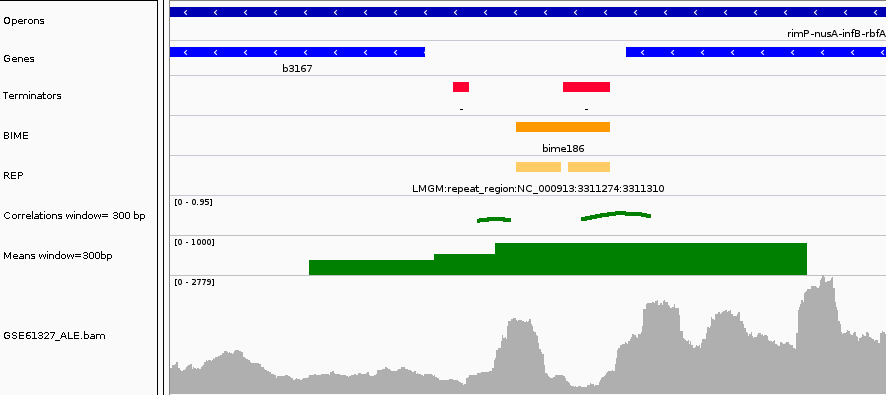
\includegraphics[scale=0.55]{figures/igv_profil.png}}
\caption{\textbf{Visualisation des changements de couverture obtenus par la méthode de corrélation des profils.} L'opéron est de couleur en bleu foncée, les gènes sont bleu clair, les terminateurs de transcription en rouge, les BIME sont représentées en orange foncé, les REP en orange clair. Le diagramme de barres en vert montre les profils d'expression moyens de chaque moitié de la fenêtre et la courbe en points verts indique l'évolution de la corrélation sur cette zone. Le brin sur lequel sont les éléments est indiqué par le sens des chevrons sur les gènes et opérons et par un signe sous les terminateurs. Dans cet exemple, le changement d'expression indique une diminution du niveau d'expression sur le brin complémentaire avec la BIME chevauchant le premier terminateur où se situe le 1\up{er} point de cassure et un 2\up{ème} situé juste après la BIME ce qui explique le diagramme de barre à 3 niveaux (2 diagrammes de barres se chevauchant).}
\label{fig:igv_profil}
\end{figure}

Le choix de la taille de la fenêtre glissante a été motivé par plusieurs raisons, suite à des essais nous sommes arrivés aux conclusions qu'une fenêtre trop petite (100 pb) présente une sensibilité trop importante aux variations locales dues au manque d'uniformité de la couverture (voir \nameref{uniformite_couverture}), alors qu'une fenêtre de taille trop grande (500 pb) produit une perte de sensibilité en lissant les couvertures de chaque moitié de la fenêtre. L'idée étant de rechercher le changement d'expression en ayant des informations sur la couverture moyenne des gènes flanquant la BIME, les informations d'annotation (Figure \autoref{fig:operonFigB}) nous indiquent que la majorité des régions inter-géniques contenant des BIME mesurent dans les 150 pb. Comme la BIME se situe dans la plupart des cas proche d'un des deux gènes nous avons opté pour une fenêtre de taille 300 pb pour couvrir à la fois un des gènes et la RIG. Les espaces génomiques des BIME ont été augmentés de 40 pb de chaque côté (taille moyenne d'une REP) afin de capter les points de cassure se situant aux limites de la BIME. Le seuil de la p-valeur ainsi que de niveau de changement d'expression ont été repris de la publication. Après avoir réalisé une série d'essais, la valeur du seuil de corrélation a été ajusté de 0.7 à 0.5 afin de détecter un nombre de points de cassure suffisamment important, avec une corrélation encore définie comme forte, sans pour autant obtenir trop de faux positifs. Ce choix se justifie du fait que par rapport à l'article originel nous avons augmenté la taille de la fenêtre de 100 à 300 pb, nous disposons donc de 200 points de couverture en plus pour établir la corrélation tout en conservant une p-valeur très basse pour ce test de corrélation. 

\begin{SCfigure}[][h!]
\fbox{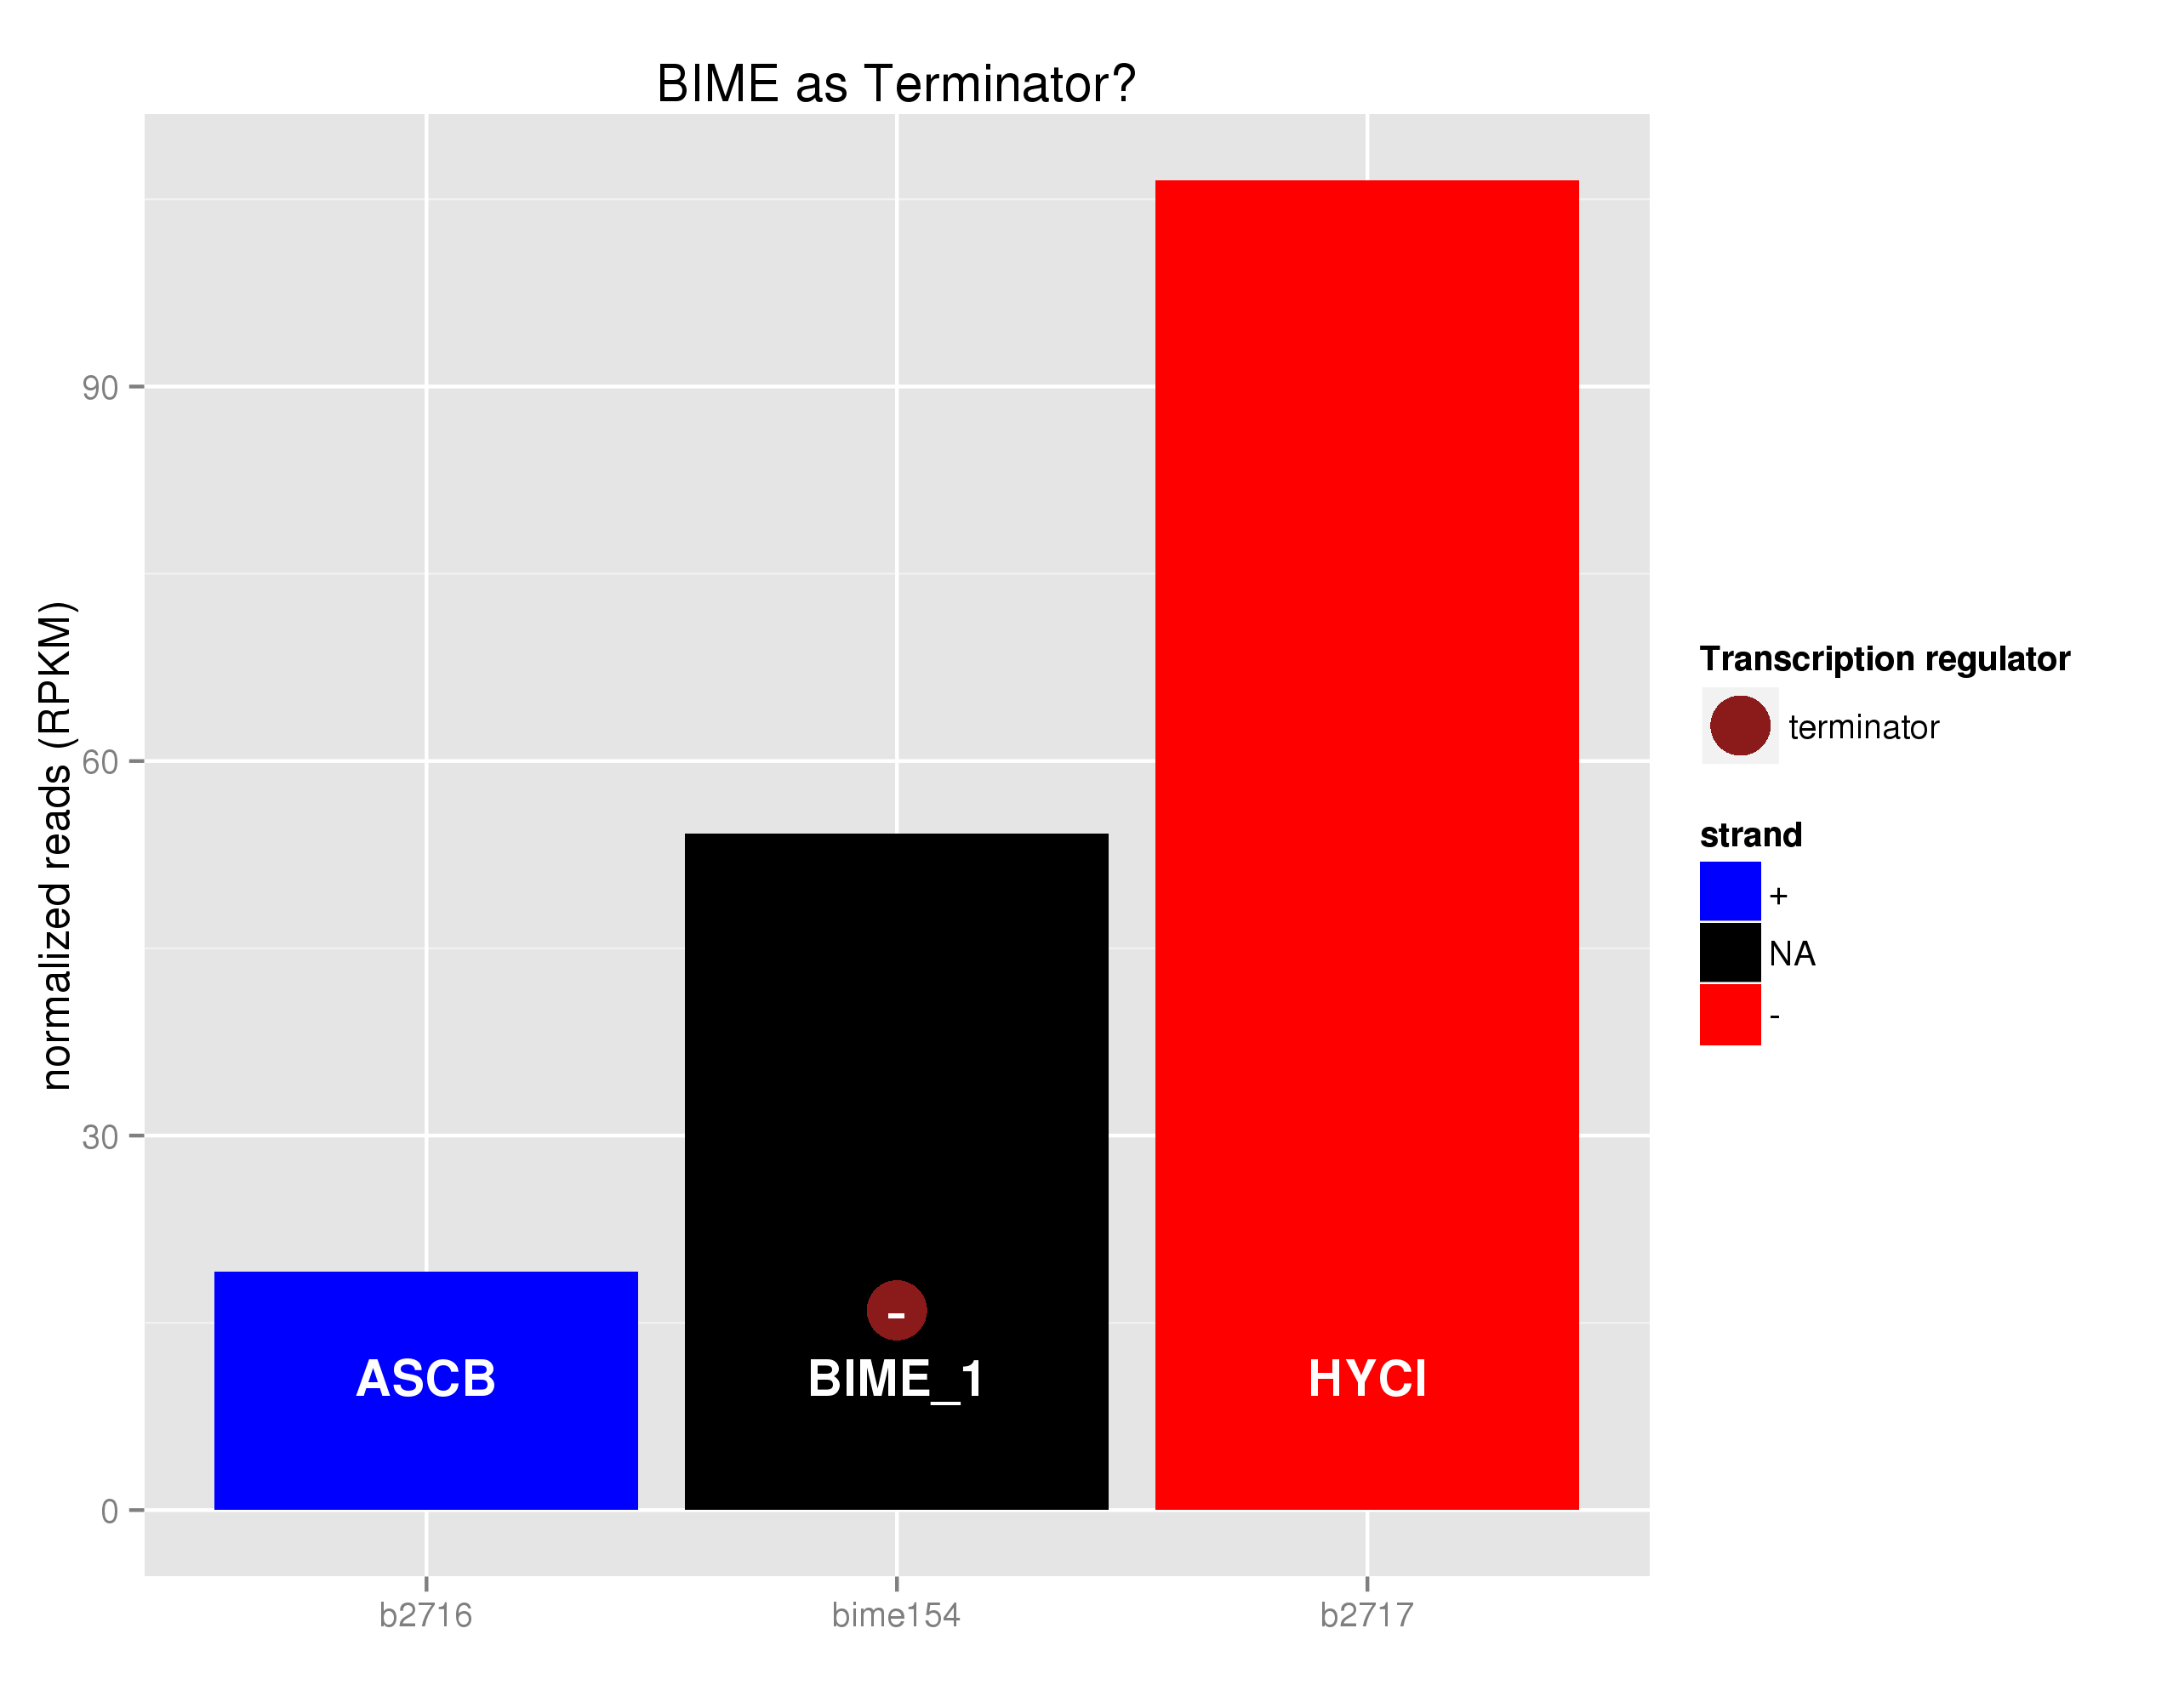
\includegraphics[scale=0.5]{figures/profil_plot.png}
\caption{\textbf{Résultat de corrélation de profils.} Les niveaux d'expression des gènes encadrant la BIME et de cette dernière sont représentés par diagrammes de barre (même cas que pour la \autoref{fig:igv_profil}). La couleur du diagramme indique le sens de transcription de l'élément, bleu pour le brin direct, rouge pour le brin complémentaire et noir lorsque aucun brin est défini. La présence d'éléments de régulation dans la RIG est représentée par des ronds de couleur verte pour les promoteurs et rouge pour les terminateurs de transcription avec un symbole '+' ou '-' pour indiquer le sens du brin de cet élément. La représentation est schématique et ne donne pas d'information sur la position exacte de ces éléments ni sur leur nombre.}
\label{fig:profil_plot} }
\end{SCfigure}

Sur un ensemble de positions consécutives dont les corrélations sont significatives et sont situées sur l'espace génomique de la BIME, celle dont la corrélation est la plus élevée sera définie comme position de changement d'expression. Deux types de fichiers sont générés au format \texttt{bedgraph} pour une visualisation sur un Genome Browser, le premier sous forme de diagramme de barre représentant les couvertures moyennes des deux parties de la fenêtre, le second représentant l'évolution de la corrélation sur la zone (\autoref{fig:igv_profil}). Une visualisation des niveaux d'expression des 2 gènes et de la BIME est également générée sous forme de diagramme de barres avec les informations de sens et du type de la BIME (\autoref{fig:profil_plot}).

Cette méthode de détection de points de cassures dans la couverture est applicable à tous les gènes du génome, mais nous nous sommes concentrés sur les résultats localisés dans les opérons visibles dans le \autoref{table:profil}.

\begin{table}[h!]
\centerline{
\begin{tabular}{|l|c|c|}
  \hline
  \rowcolor{Gray} Jeux de données &\begin{tabular}{c} Nb. de points\\de cassure détectés \end{tabular} & \begin{tabular}{c}Présence de\\promoteurs et/ou terminateurs\end{tabular}\\ 
  \hline
  GSE61327\_ALE & 12 & 5/12  \\  
  \hline
  HS-15min & 5 & 0/5 \\ 
  \hline
  M-P4h & 5 & 2/5  \\
 \hline
\end{tabular}}
\caption{\textbf{Résultats de l'étude par la méthode de corrélation sur les gènes des opérons flanquant une BIME.} La 2\up{nde} colonne indique le nombre de points de cassures dans la couverture détectés sur une BIME. La 2\up{ème} indique combien de RIG contiennent également des promoteurs et/ou terminateurs pouvant jouer un rôle sur le changement de niveau d'expression.
\label{table:profil}}
\end{table}

Pour les données GSE61327\_ALE, 12 points de cassures sont détectés sur les 32 opérons contenant des gènes DE flanquant une BIME et 5 d'entre eux pourraient être sous l'effet d'un promoteur ou terminateur de transcription. Pour les 2 autres jeux de données, 5 points de cassure sont détectés et seul l'expérience M-P4h pourrait avoir 2 points de cassure causés par la présence d'un promoteur ou un terminateur.

\section*{Approche globale, segmentation}

En reprenant la méthode décrite dans la partie \nameref{methode_segmentation}, nous avons fixé le paramètre $K$ à 4 segments maximum donc 3 points de cassure de façon à vérifier la présence éventuelle de plusieurs de ces points sur la RIG.
Dans notre étude, nous nous intéressons aux positions de ces points de cassures pour nos régions d'intérêt, définis de la même manière que précédemment, lorsqu'au moins un des deux gènes possède une couverture supérieure à 10. Les résultats sont croisés avec la présence de promoteurs ou de terminateurs de transcription dans la RIG et si les deux gènes appartiennent à un opéron, un test  statistique sur la différence d'expression est réalisé avec la même méthodologie que pour la partie~\nameref{expression_operon}.

\begin{SCfigure}[][h!]
\fbox{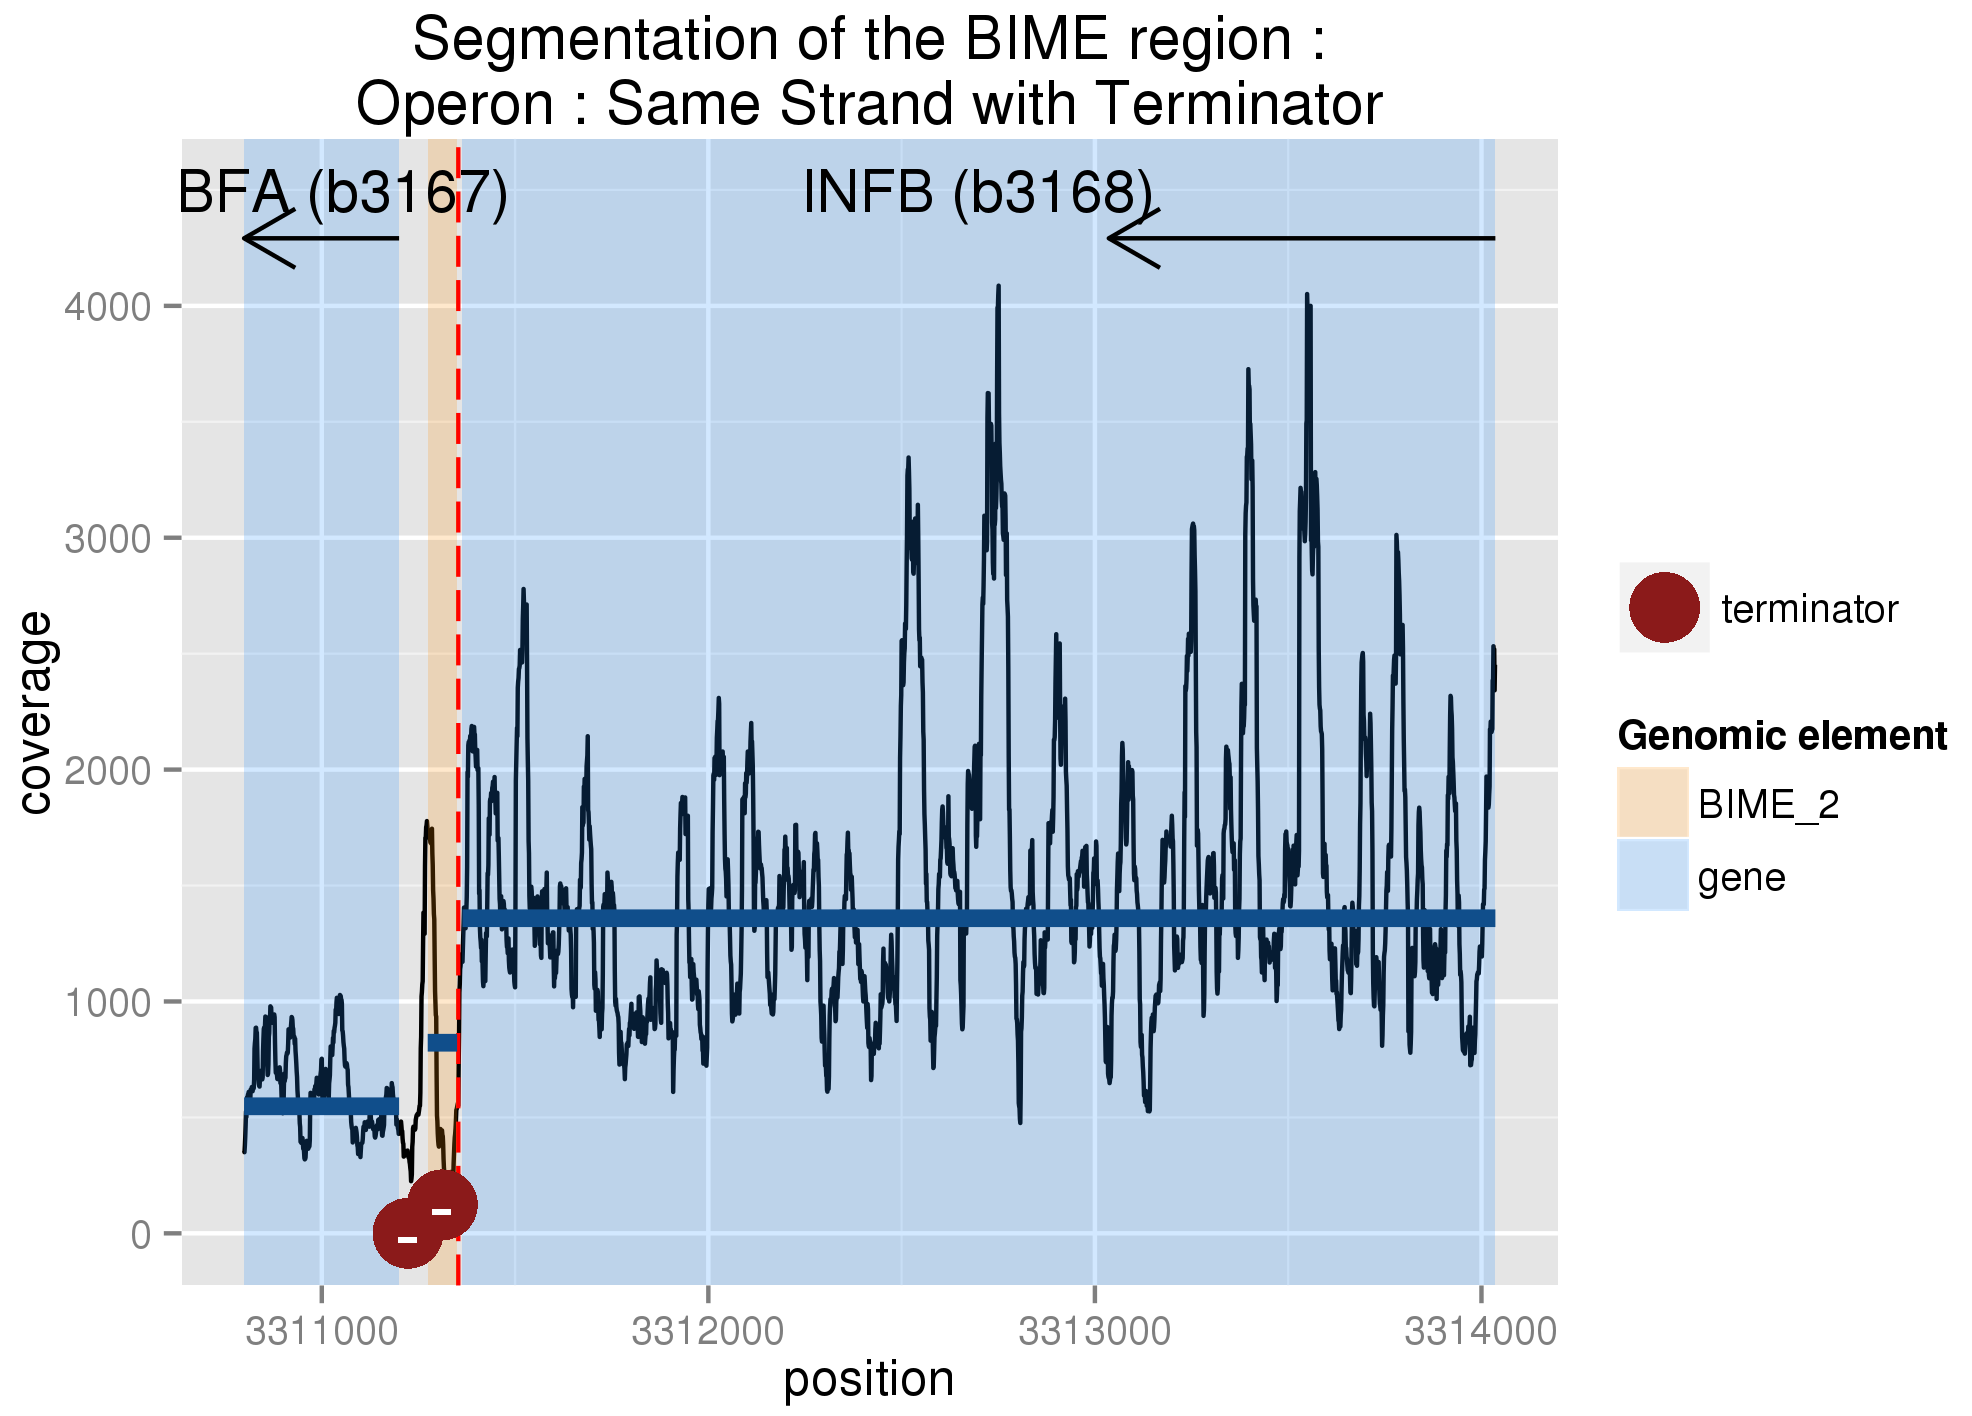
\includegraphics[scale=0.75]{figures/segmentation.png}
\caption{\textbf{Résultat de segmentation pour $K_{max} \mathord{=} 4$.} Les gènes sont symbolisés par les zones bleues, leur sens de transcription par les flèches noires. La BIME est représentée par la zone orange et sa classe est précisée dans la légende (Genomic element). Les promoteurs sont représentés par des points verts et les terminateurs par des points rouges, leur sens affichés par les symboles '+' ou '-' sur ces points. La courbe noire représente la couverture sur la région et les barres bleues horizontales indiquent les couvertures moyennes des éléments génomiques. Les points de cassure dans la couverture, déterminés par la segmentation, sont matérialisés par des lignes rouges verticales en pointillés.}
\label{fig:segmentation} }
\end{SCfigure}

L'analyse renvoie une représentation graphique de la couverture de ces régions avec les positionnements des gènes et de la BIME, ainsi que des promoteurs et terminateurs éventuels. Une classification est faite en fonction du sens des gènes et de l'impact des promoteurs et terminateurs de transcription sur la couverture (\autoref{fig:segmentation}). Les résultats de la segmentation sont présentés dans le \autoref{table:segmentation}, bien que cette méthode soit applicable à l'ensemble du génome d'\textit{E. coli}, nous nous sommes concentré sur les opérons.

\begin{table}[h!]
\centerline{
\begin{tabular}{|l|c|c|c|c|}
  \hline
  \rowcolor{Gray} Jeux de données &\begin{tabular}{c} Nb. d'opérons avec\\un point de cassure\\détecté dans\\la RIG avec BIME\end{tabular} & \begin{tabular}{c}Présence de\\promoteurs et/ou\\ terminateurs\end{tabular} & \begin{tabular}{c} Nb. de points\\ de cassure\\sur la BIME\end{tabular} & \begin{tabular}{c} Nb. de points \\de cassure\\sur la BIME sans \\promoteur ou \\terminateur\end{tabular}\\ 
  \hline
  GSE61327\_ALE & 15 & 7/15 & 12/15 & 8/15 \\  
  \hline
  HS-15min & 5 & 1/5 & 5/5 & 4/5 \\ 
  \hline
  M-P4h & 2 & 0/2 & 2/2 & 2/2 \\
 \hline
\end{tabular}}
\caption{\textbf{Résultats de l'étude par la méthode de segmentation sur les gènes des opérons flanquant une BIME.} La 2\up{nde} colonne indique le nombre de points de cassures dans la couverture, la 3\up{ème} indique combien de RIG contiennent également des promoteurs et/ou terminateurs pouvant jouer un rôle sur le changement de niveau d'expression, la 4\up{ème} combien de points de cassures sont situés sur la BIME et la dernière combien de ces points de cassure sont dans des RIG sans promoteurs ou terminateurs.
\label{table:segmentation}}
\end{table}

Les résultats obtenus par la segmentation sont proches de ceux de la recherche de changement de niveau d'expression du \autoref{table:expression} sauf pour le jeux de données M-P4h pour lequel très peu de changements de niveau d'expression sont détectés dans les opérons. La plupart des points de cassure sont détectés sur les BIME, ce qui va dans le sens d'une implication de ces dernières dans la régulation transcriptionnelle. Pour le jeu de données GSE61327\_ALE, la présence de promoteurs et de régulateurs est plus importante et seuls 3 cas sur 15 ont un point de cassure situé en dehors de la BIME (voir annexe \ref{annexeSegmentation}).

\section*{Évolution des structures des BIME}
Les résultats des trois méthodes précédentes ont été croisés afin de sortir les couples de gènes flanquant une BIME dans un opéron retrouvés par chacune d'elles. Nous observons 11 couples pour le jeux de données GSE61327\_ALE, 3 pour HS-15min et un seul pour M-P4h (Annexe \ref{annexeVenn}). Nous nous sommes intéressés aux 11 résultats produits par GSE61327\_ALE que nous avons traités par la méthode de reconstruction des états ancêtres.

\begin{table}[h!]
\centerline{
\begin{tabular}{|l|c|c|c|}
  \hline
  \rowcolor{Gray} Couples de gènes & \begin{tabular}{c}Nombre d'espèces\\dans le cluster \end{tabular} & \begin{tabular}{c}Énergie de la\\structure secondaire \end{tabular} & \begin{tabular}{c}Delta d'énergie avec\\l'état ancêtre à la racine \end{tabular}\\ 
  \hline
  GABT\_GABP & 25 & -44.8 & -5.6 \\  
  \hline
  HYDN\_HYPF & 45 & -47 & +2.1 \\
  \hline
  INFB\_RBFA & 32 & -40.1 & +0.8 \\
  \hline
\end{tabular}
}
\caption{\textbf{Résultats de la reconstruction des états ancêtres et de l'étude des structures secondaires.} 
\label{table:segmentation}}
\end{table}






\chapter*{Discussion}




\end{onehalfspace}


% affichage du glossaire
\renewcommand{\thepage}{}
\printglossary[type=\acronymtype ,title=Glossaire]

%\bibliographystyle{unsrtnat}
\bibliography{biblio_rapport}

% annexes
\appendix

\chapter{}
\label{annexeCode}

Décompression du fichier au format \texttt{SRA} au format \texttt{Fastq}, puis contrôle qualité des reads.
\lstset{language=sh, commentstyle=\color{ForestGreen}} 
\begin{lstlisting}[frame=single]
# Decompression
fastq-dump -Z file.sra > file.fastq
# Controle qualite
fastqc file.fastq
\end{lstlisting}

Alignement des reads des fichiers \texttt{Fastq} sur le génome de référence, puis conversion du fichier \texttt{SAM} en fichier \texttt{BAM}. Tri du fichier \texttt{BAM} en fonction des positions génomiques. 
\lstset{language=sh, commentstyle=\color{ForestGreen}} 
\begin{lstlisting}[frame=single]
# Indexation du genome de reference
bwa index ref.fasta
# Alignement avec l'algorithme MEM de BWA
bwa mem ref.fasta file.fastq > aln.sam
# Conversion du SAM en BAM et application des filtres
# (-q 30: mapping minimal, -F 2048: pas de sequence chimeriques).
samtools view -Sbh -q 30 -F 2048 aln.sam > aln.bam
# Tri en fonction des positions genomiques
samtools sort aln.bam aln_sorted
\end{lstlisting}

Indexation du fichier \texttt{BAM} trié pour visualisation sur un Genome Browser. Fusion des différents fichiers \texttt{BAM} des réplicats en un seul fichier \texttt{BAM}.
\lstset{language=sh, commentstyle=\color{ForestGreen}} 
\begin{lstlisting}[frame=single]
# Indexation du fichier d'alignement
samtools index aln_sorted.bam
# Fusion des replicats.
samtools merge merged.bam aln_sorted_1.bam aln_sorted_2.bam \
aln_sorted_3.bam
\end{lstlisting}

Utilisation des BEDtools pour obtenir la couverture base par base sur une région d'intérêt.
\lstset{language=sh, commentstyle=\color{ForestGreen}}  
\begin{lstlisting}[frame=single]
# Couverture base par base.
bedtools coverage -abam merged.bam -b regionOfInterest.bed \
-d > unsorted_cov_perBase.bed
# Tri en fonction de la position genomique puis de la position 
# des bases dans chaque transcrit
sort -k2 -k7 -n unsorted_cov_perBase.bed | uniq > \
cov_perBase_strandToFix.bed
# Remplacement des '.' par des '*' dans la colonne des brins 
# pour l'utilisation sous R
awk 'BEGIN{OFS = "\t"} {gsub(/\./,"*",$6); print }' \
cov_perBase_strandToFix.bed > cov_perBase.bed
\end{lstlisting}

\chapter{}
\label{annexeOperon}
\begin{figure}[!h]
\centerline{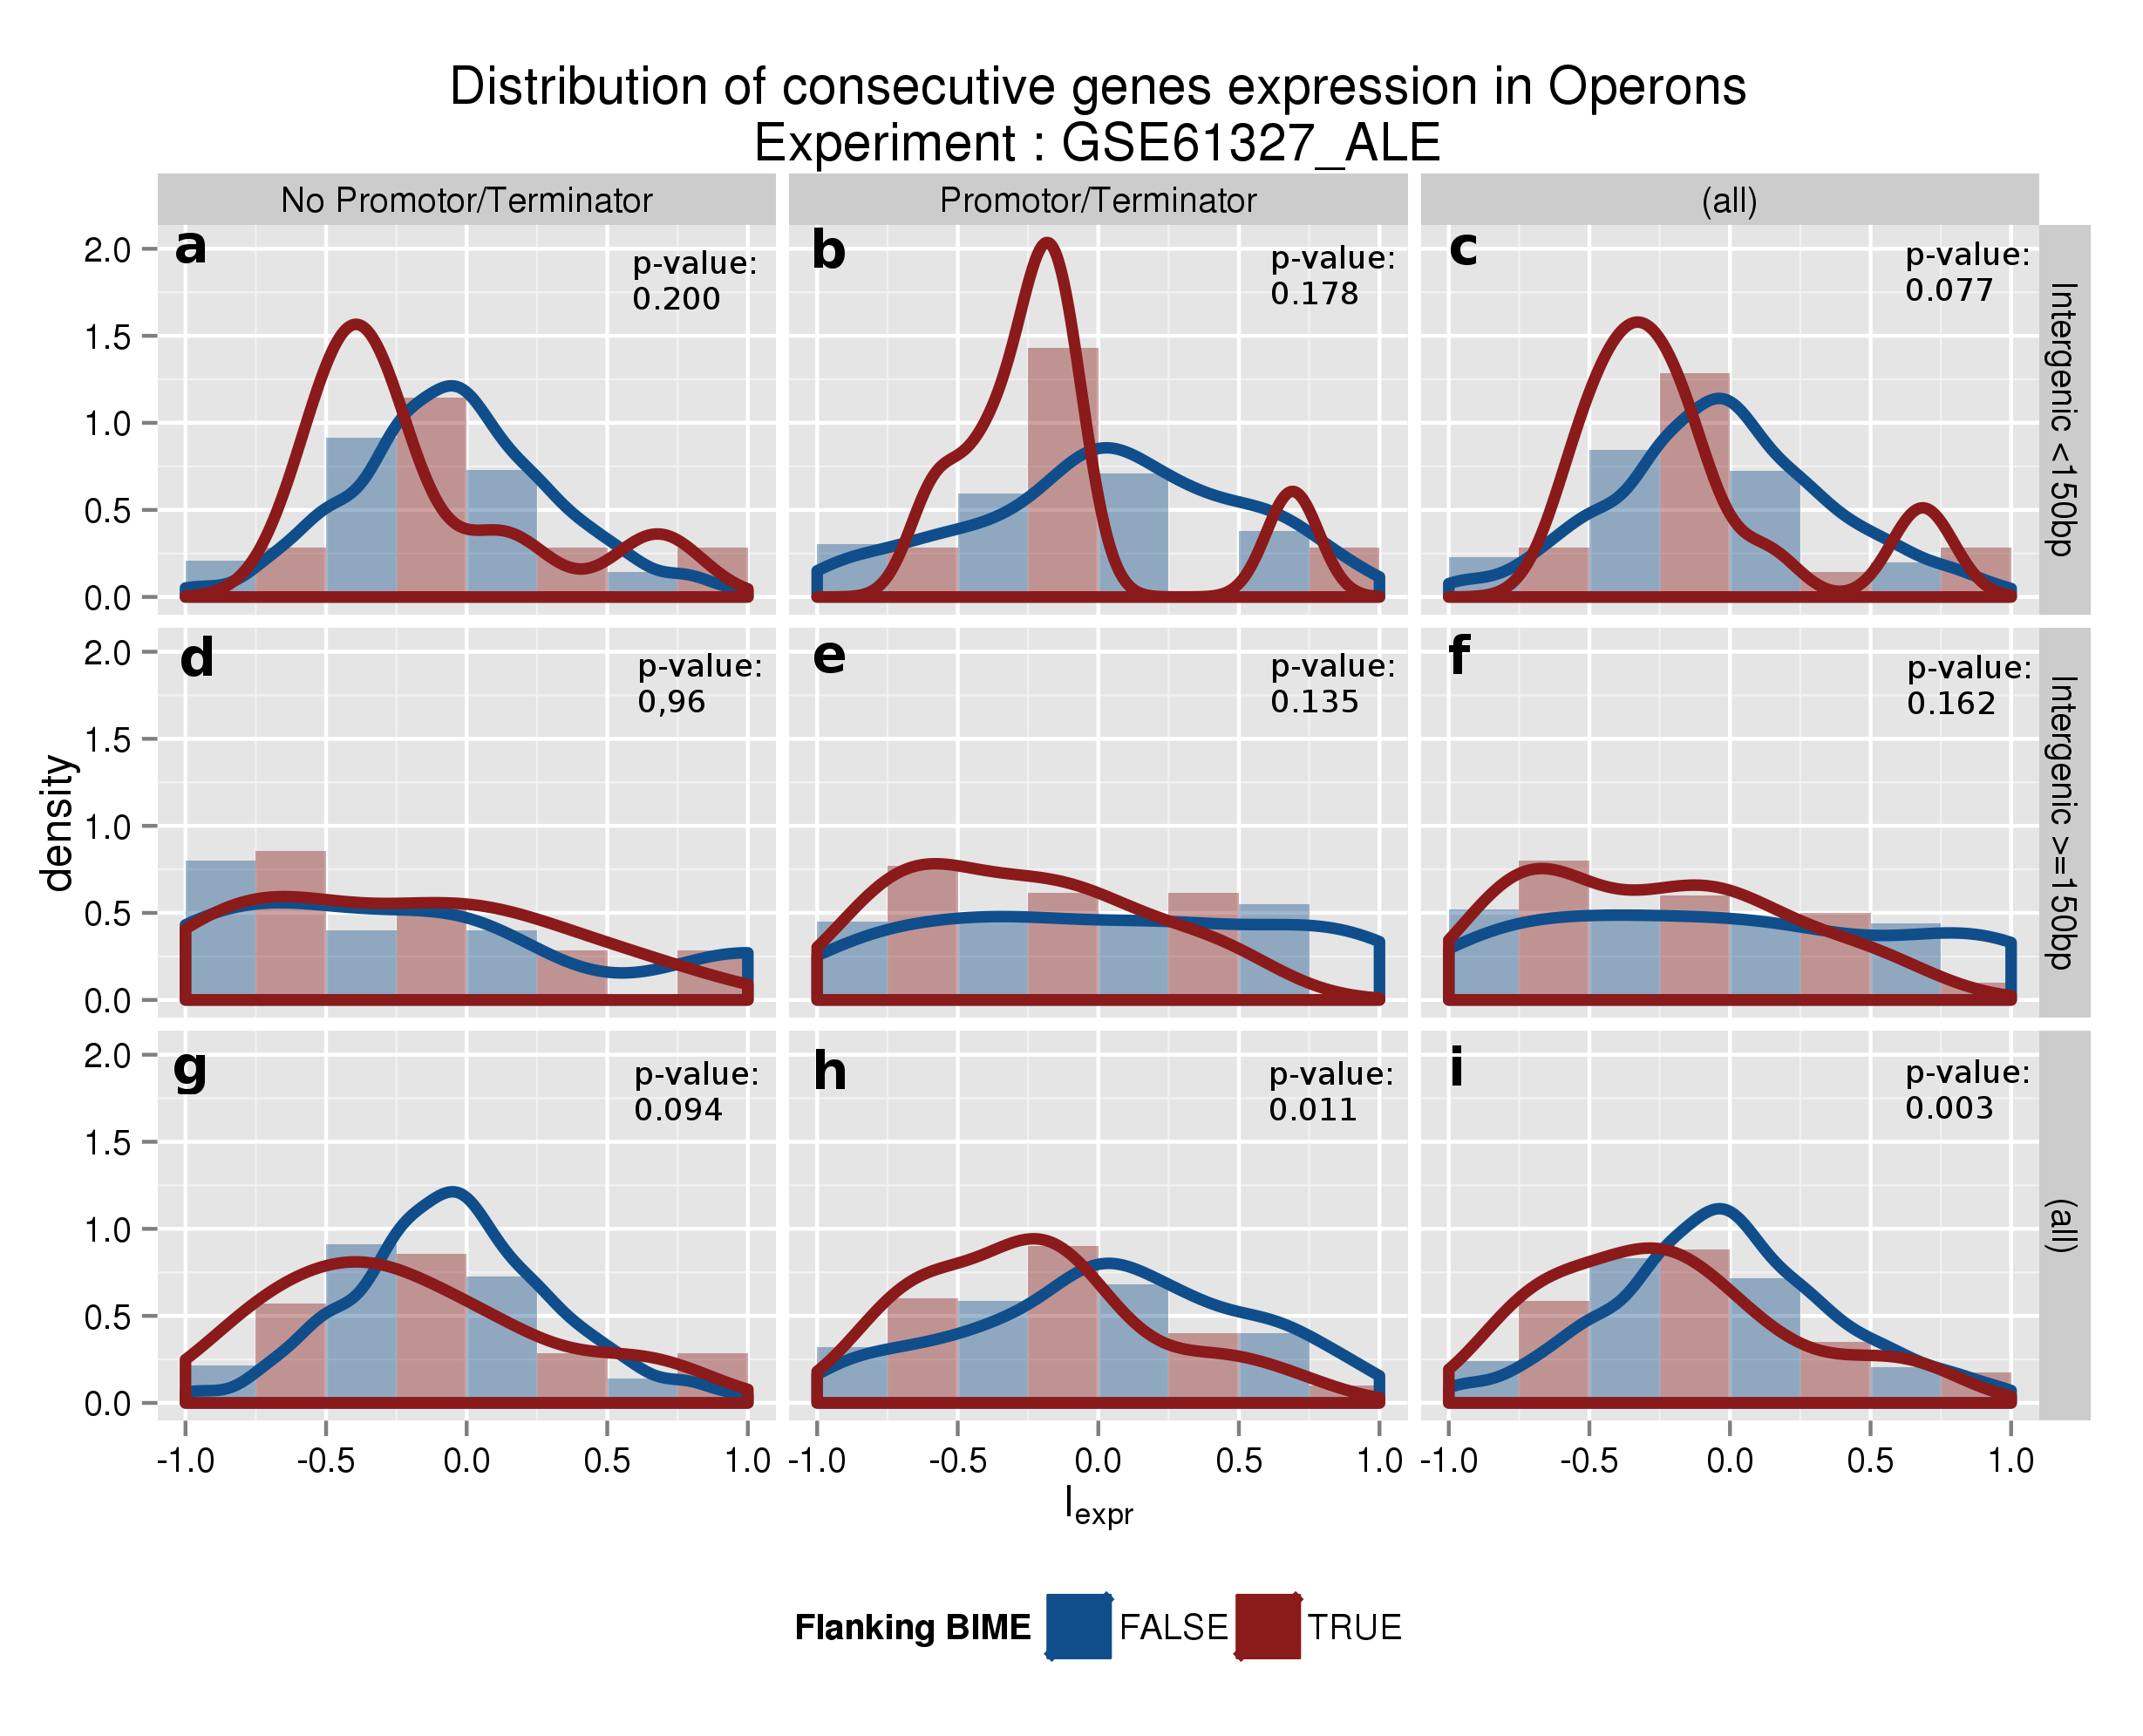
\includegraphics[scale=0.7]{figures/supData/genesOperon_histoDens_GSE61327_ALE.png}}
\caption{\textbf{Niveau d'expression des gènes consécutifs dans les opérons pour le jeux de données GSE61327\_ALE.}}
\end{figure}

\begin{figure}[!h]
\centerline{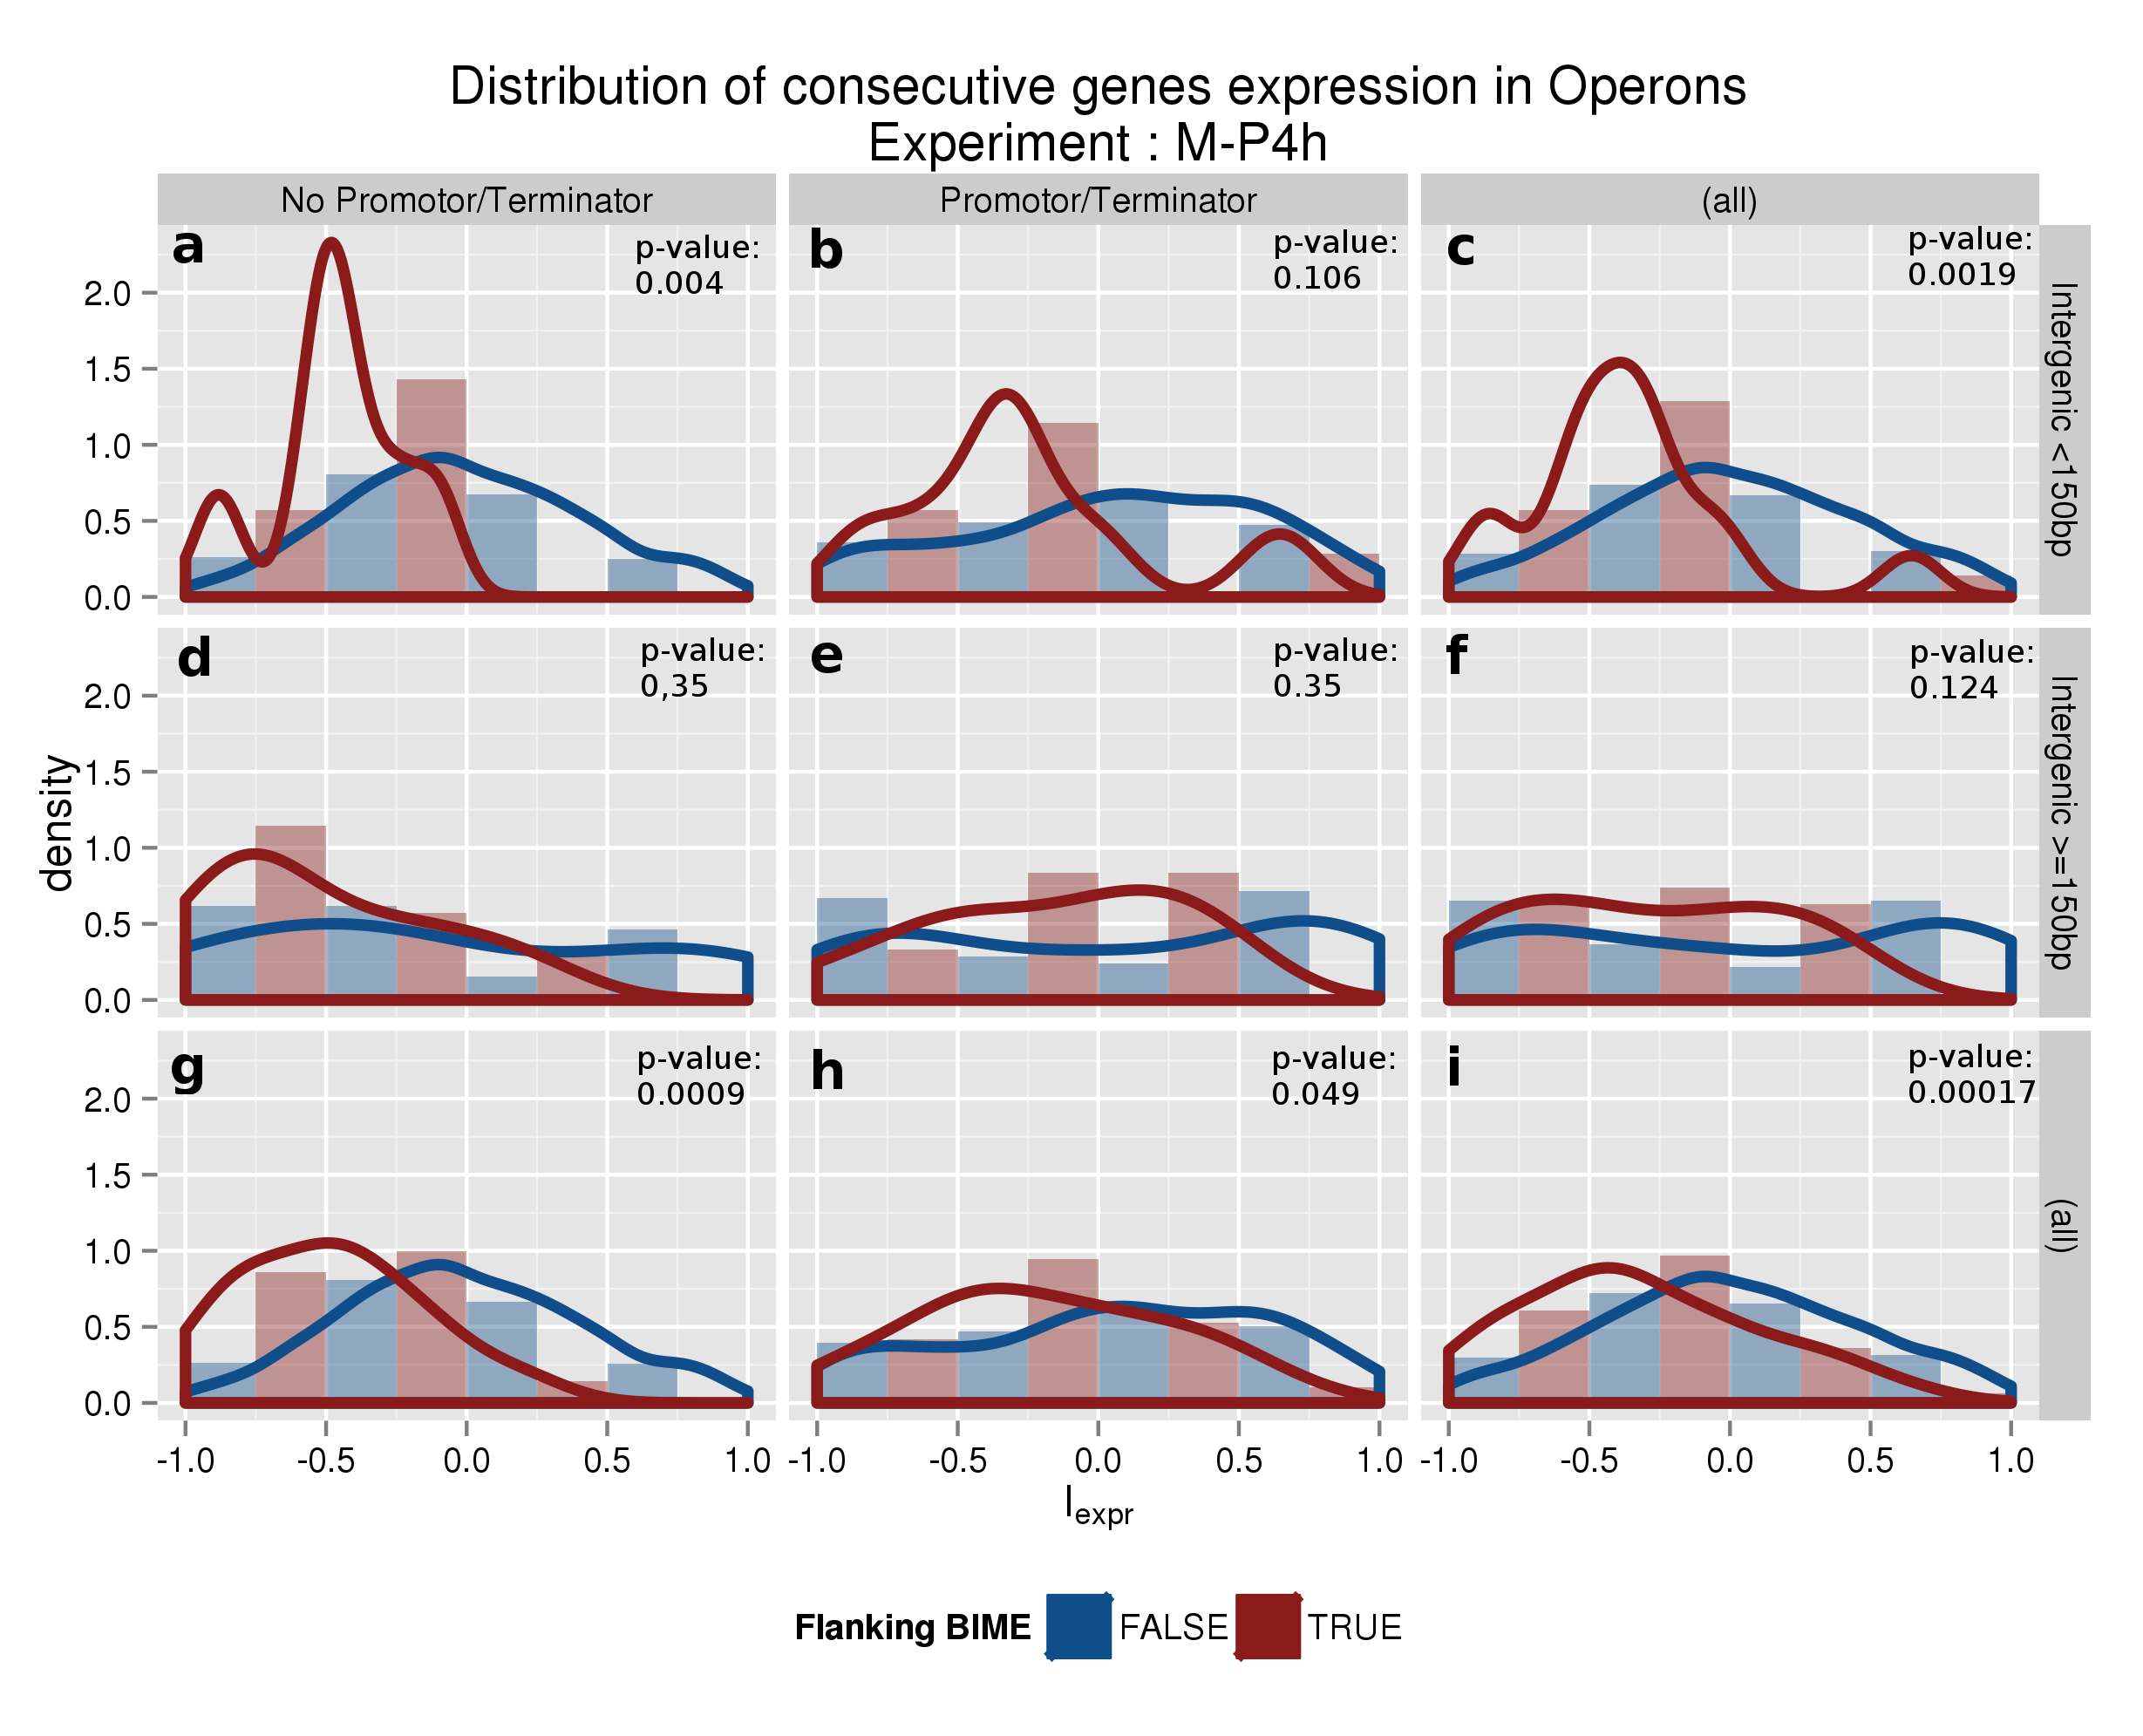
\includegraphics[scale=0.7]{figures/supData/genesOperon_histoDens_M-P4h.png}}
\caption{\textbf{Niveau d'expression des gènes consécutifs dans les opérons pour le jeux de données M-P4h.}}
\end{figure}

\chapter{}
\label{annexeSegmentation}
\begin{figure}[h!]
\centering
\subfigure[]{\label{fig:segmentation_A} 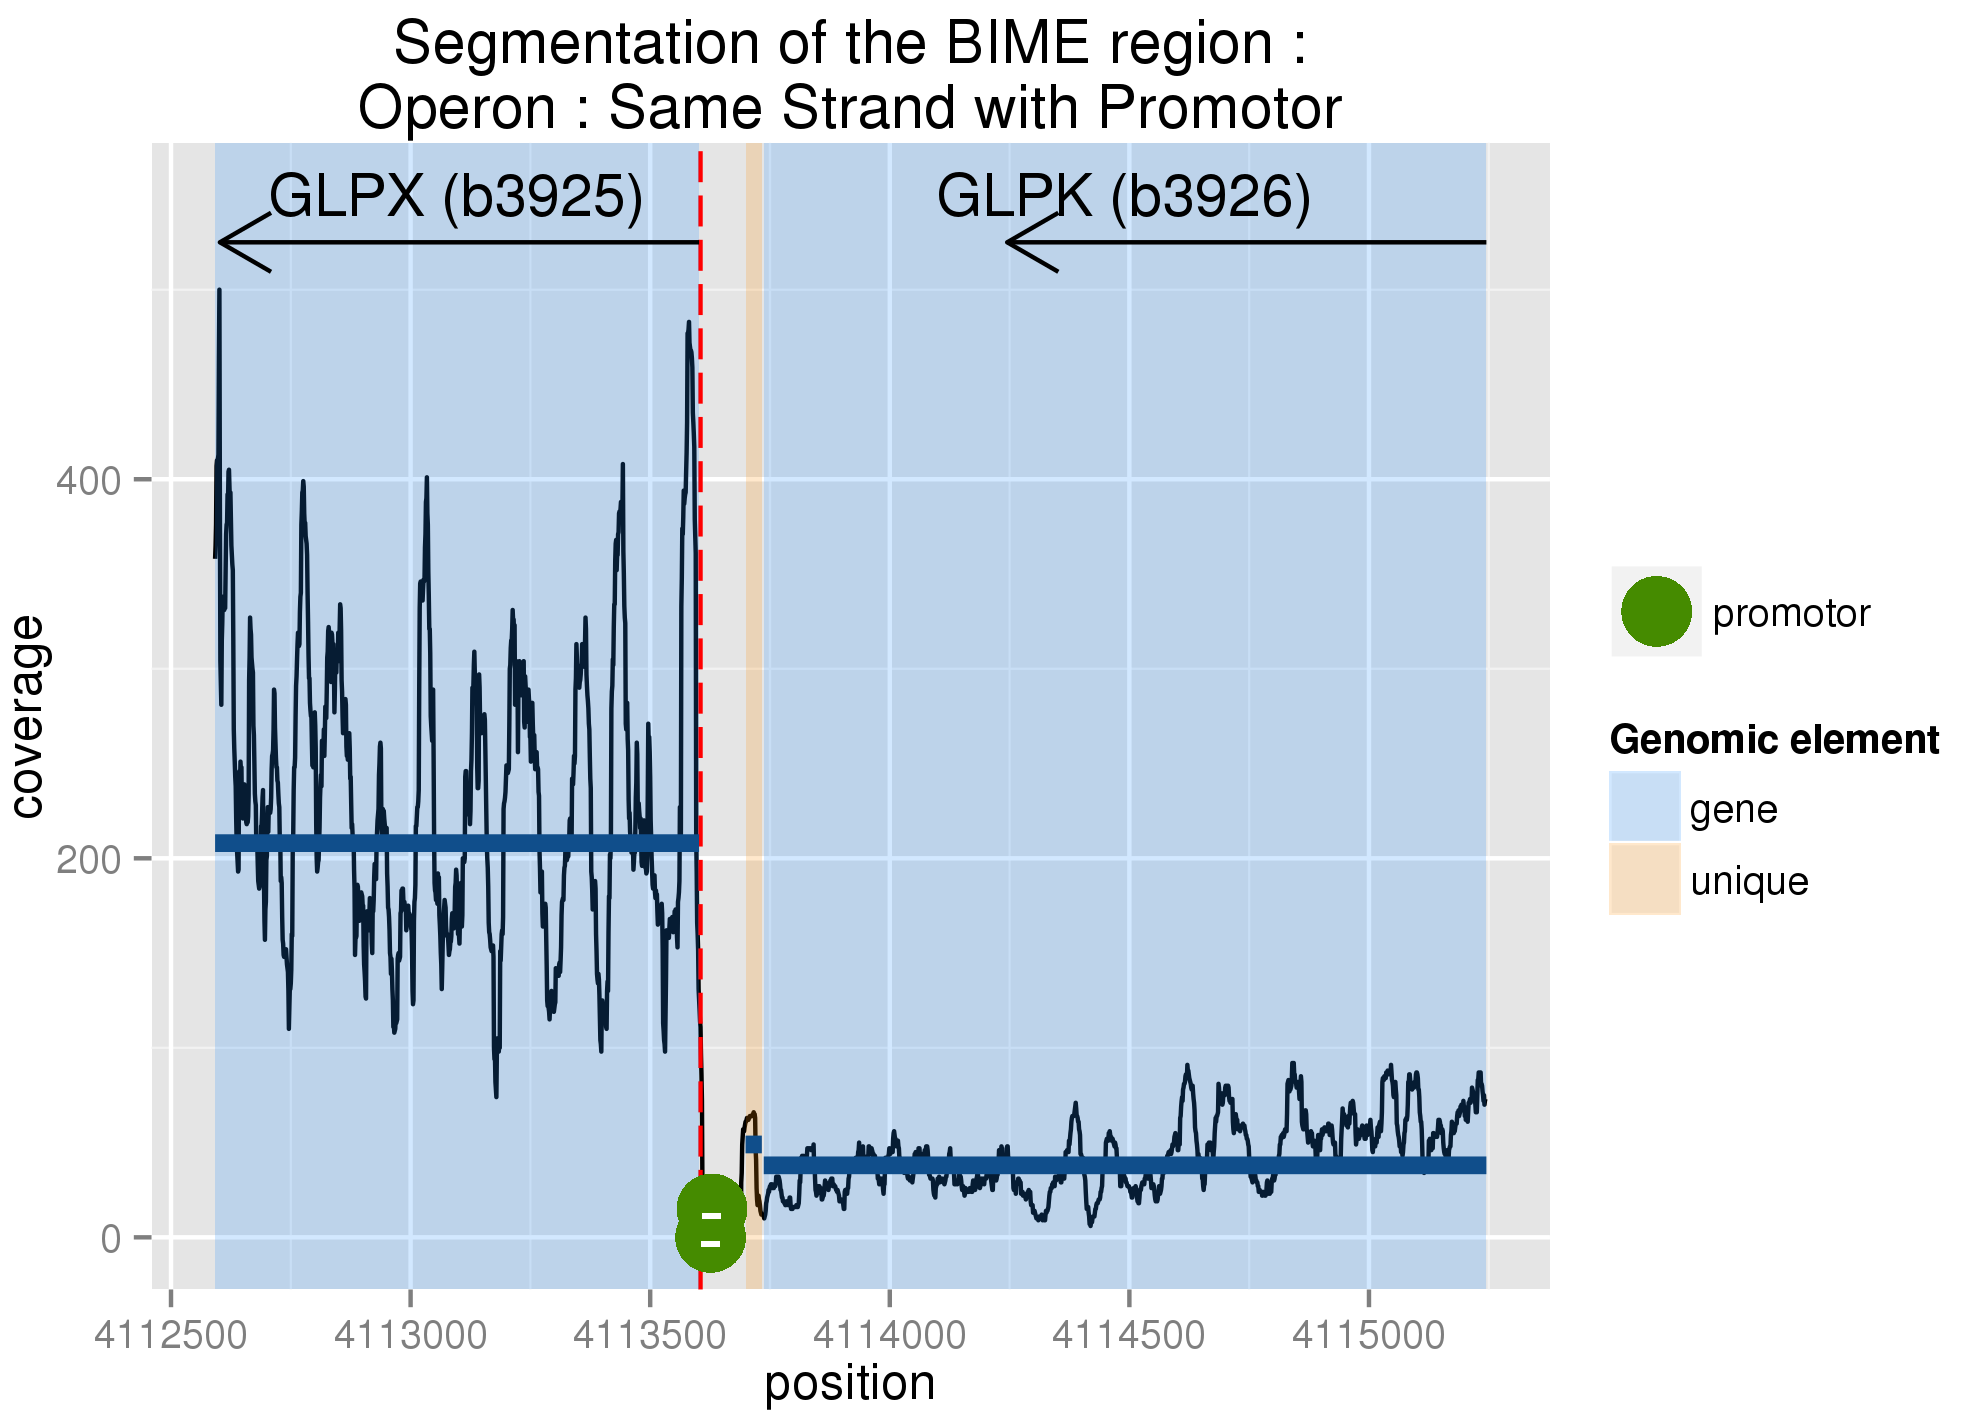
\includegraphics[scale=0.48]{figures/supData/promoSameStrand_GLPX-b3925_GLPK-b3926.png}}
\subfigure[]{\label{fig:segmentation_B} 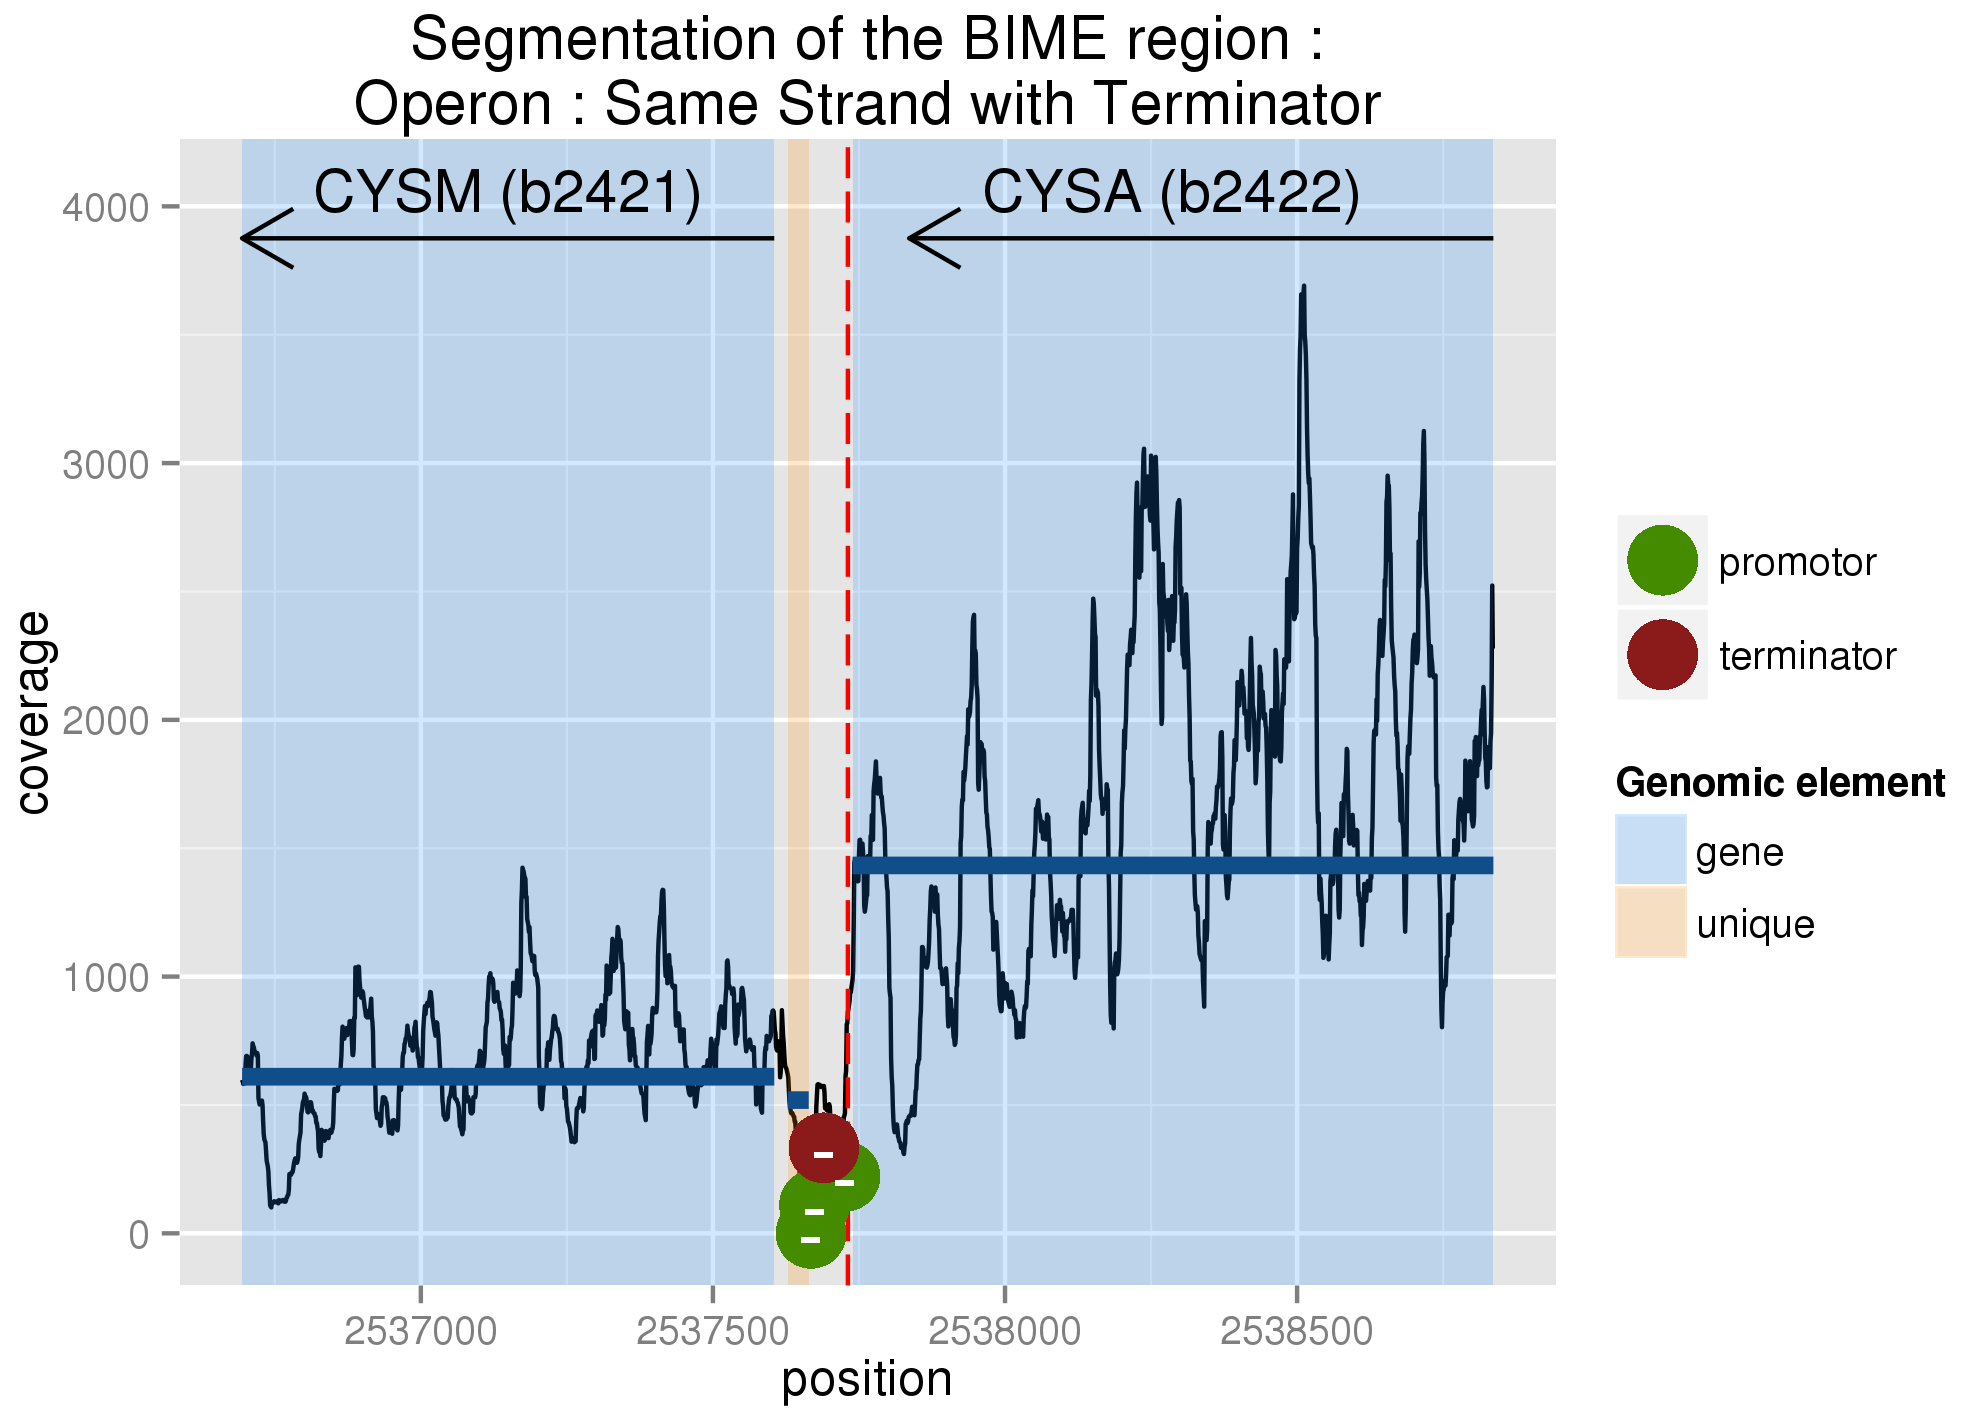
\includegraphics[scale=0.48]{figures/supData/termSameStrand_CYSM-b2421_CYSA-b2422.png}}
\subfigure[]{\label{fig:segmentation_C} 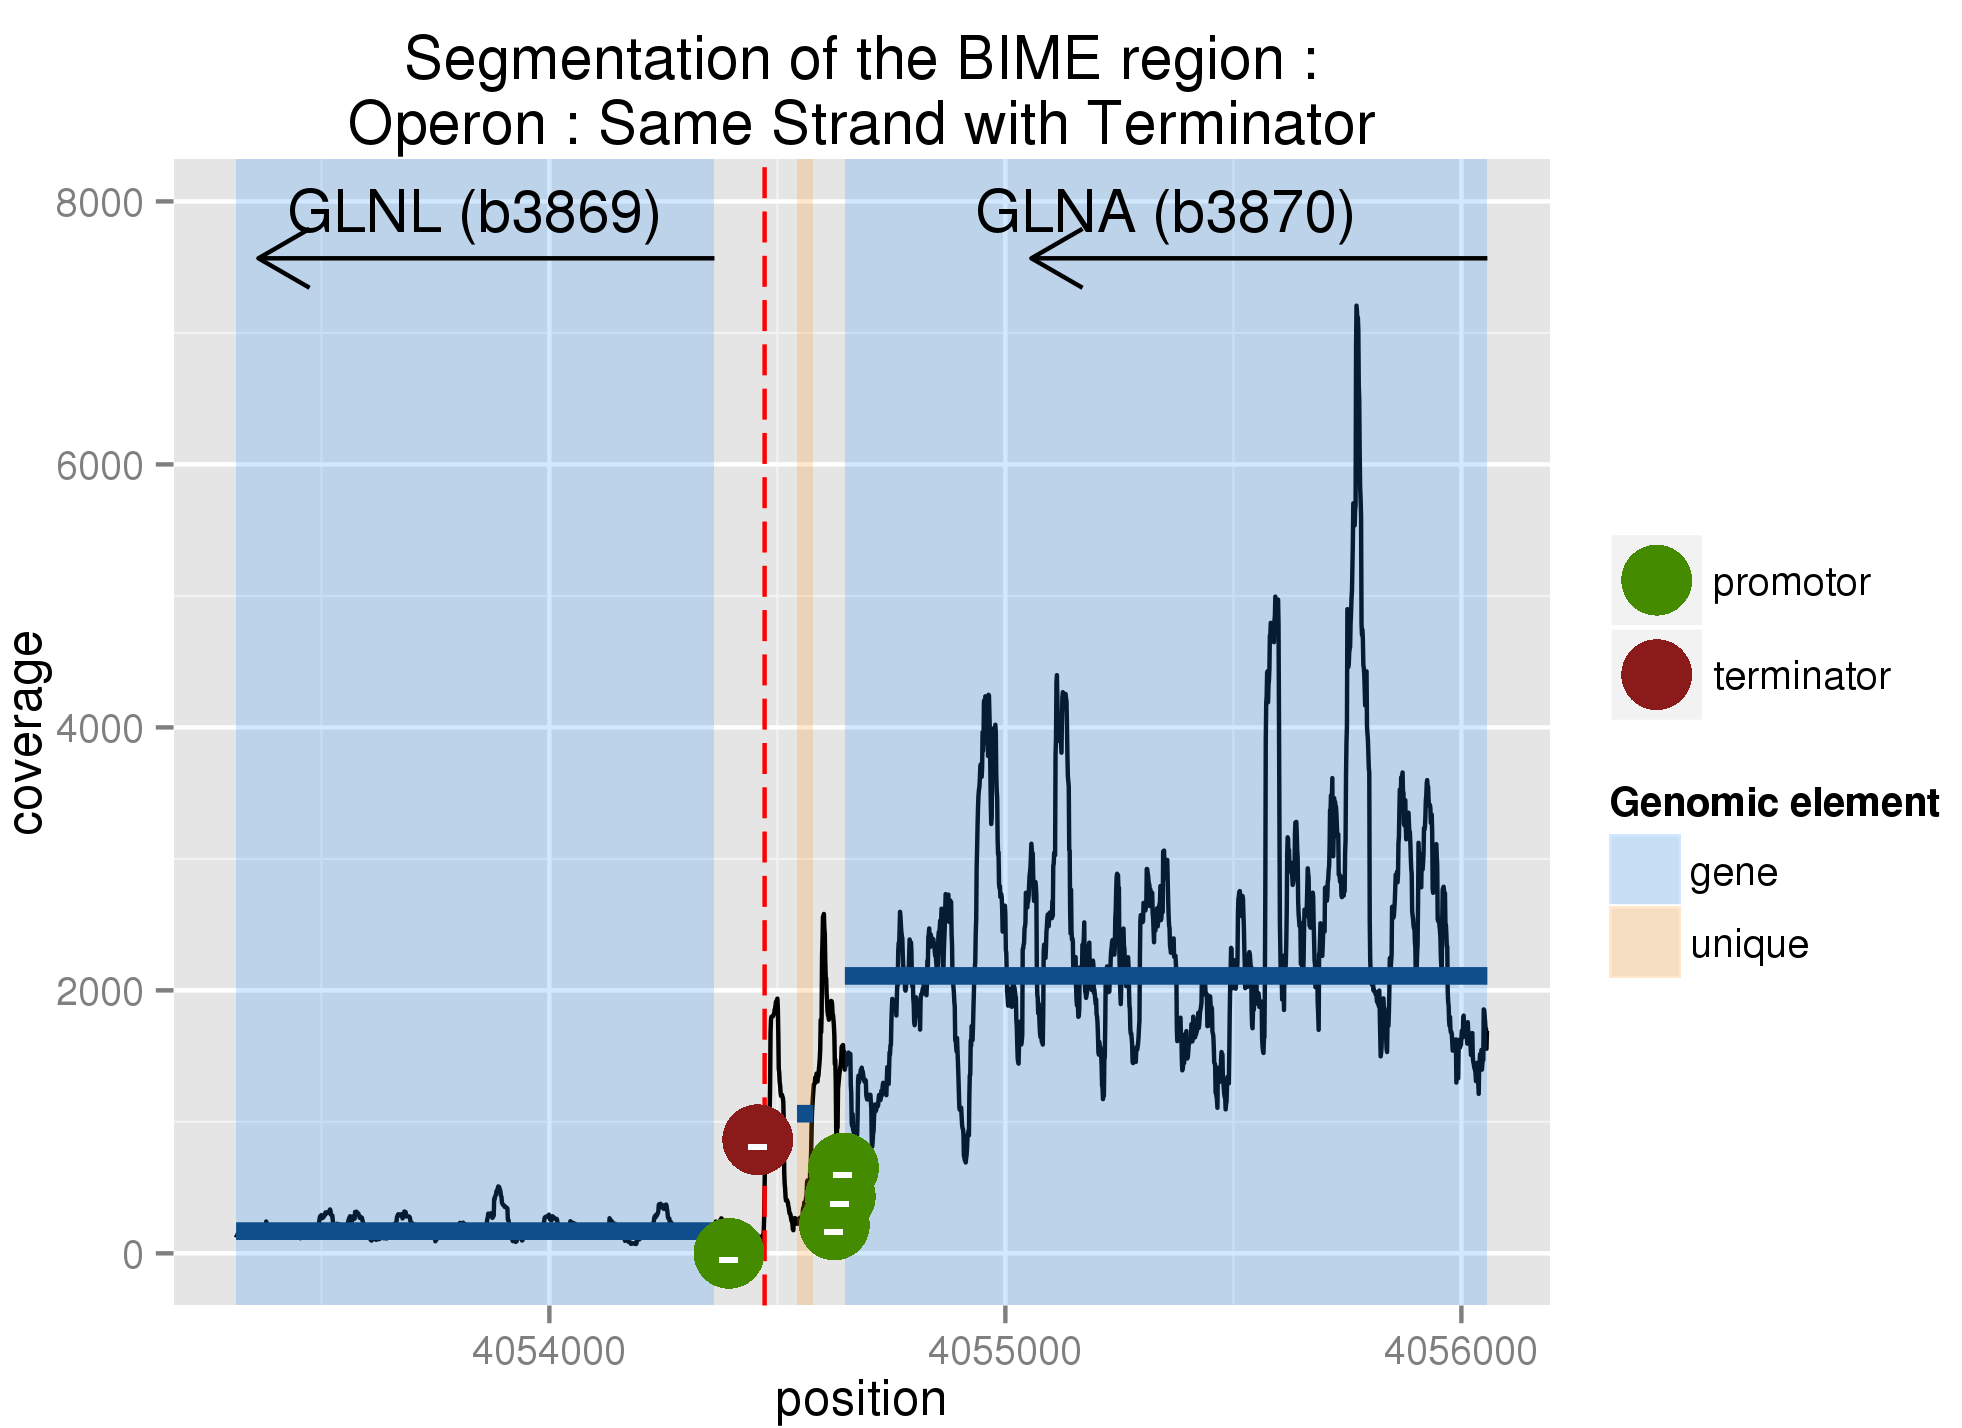
\includegraphics[scale=0.48]{figures/supData/termSameStrand_GLNL-b3869_GLNA-b3870.png}}
\caption{\textbf{(a) Opéron glpFKX.} \textbf{(b) Opéron cysPUWAM.} \textbf{(c) Opéron glnALG.} Il s'agit des 3 seuls sur 22 points de cassures détectés par la segmentation tombant en dehors de la région génomique de la BIME. Le changement de niveau d'expression est probablement dû aux promoteurs et aux terminateurs plutôt qu'aux BIME.}
\end{figure}


\chapter{}
\label{annexeVenn}
\begin{figure}[h!]
\centering
\subfigure[]{\label{fig:venn_GSE} 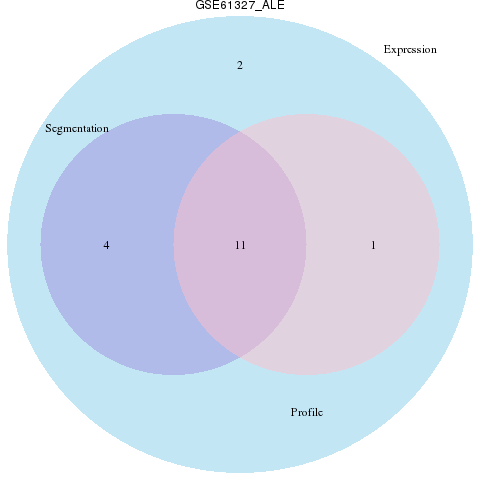
\includegraphics[scale=0.42]{figures/supData/venn_GSE61327_ALE.png}}
\subfigure[]{\label{fig:venn_HS} 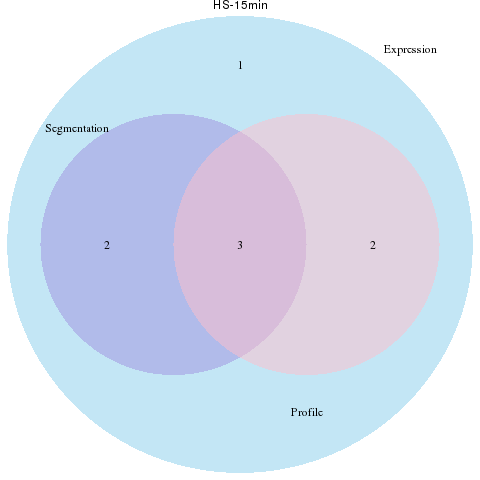
\includegraphics[scale=0.42]{figures/supData/venn_HS-15min.png}}
\subfigure[]{\label{fig:venn_MP} 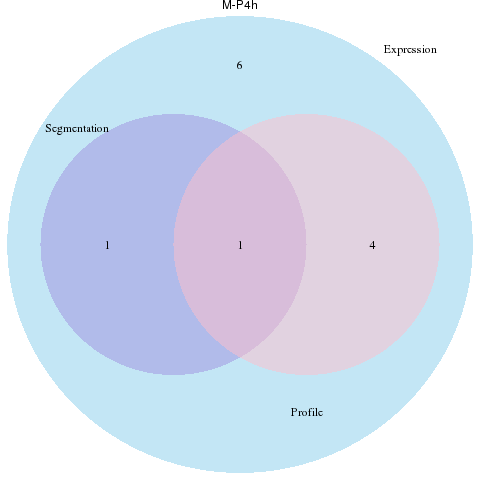
\includegraphics[scale=0.42]{figures/supData/venn_M-P4h.png}}
\caption{\textbf{Nombre de résultats trouvés pour chacune des 3 méthodes, Expression, corrélation de profils d'expression et segmentation. (a)} Données GSE61327\_ALE, 32 couples de gènes flanquant un BIME sont exprimés, pour 17 d'entre eux nous observons une DE et 11 sont retrouvés par les 3 méthodes. \textbf{(b)} Données HS-15min, 20 couples de gènes flanquant un BIME sont exprimés, pour 8 d'entre eux nous observons une DE et 3 sont retrouvés par les 3 méthodes. \textbf{(c)} Données M-P4h, 30 couples de gènes flanquant un BIME sont exprimés, pour 12 d'entre eux nous observons une DE et 1 est retrouvé par les 3 méthodes.} 
\end{figure}



\end{document}